% Institute of Computer Science thesis template
% authors: Sven Laur, Liina Kamm, Tõnu Tamme
% last change Eero Vainikko <eero.vainikko@ut.ee> 12.01.2021
%--
% Compilation instructions:
% 1. Choose main language on line 55-56 (English or Estonian)
% 2. Compile 1-3 times to get refences right
% pdflatex unitartucs-thesis-template
% bibtex unitartucs-thesis-template
%--
% Please use references like this:
% <text> <non-breaking-space> <cite/ref-command> <punctuation>
% This is an example~\cite{example}.

\documentclass[12pt]{article}

% A package for setting layout and margins for your thesis 
\usepackage[a4paper]{geometry}

%%=== A4 page setup ===
%\setlength{\paperwidth}{21.0cm} 
%\setlength{\paperheight}{29.7cm}
%\setlength{\textwidth}{16cm}
%\setlength{\textheight}{25cm}


% When you write in Estonian then you want to use text with right character set
% By default LaTeX does not know what to do with õäöu letters. You have to specify
% a correct input and font encoding. For that you have to Google the Web     
%
% For TexShop under MacOS X. The right lines are 
%\usepackage[applemac]{inputenc}
%\usepackage[T1]{fontenc} %Absolutely critical for *hyphenation* of words with non-ASCII letters.
%
% For Windows and Linux the right magic lines are   
% \usepackage[latin1]{inputenc}
% \usepackage[latin5]{inputenc}
%
\usepackage[utf8]{inputenc} %standard encoding since 2018 (can be commented out?)
\usepackage[T1]{fontenc} %Absolutely critical for *hyphenation* of words with non-ASCII letters.

% Typeset text in Times Roman instead of Computer Modern (EC)
\usepackage{times}

% Suggested packages:
\usepackage{microtype}  %towards typographic perfection...
\usepackage{inconsolata} %nicer font for code listings. (Use \ttfamily for lstinline bastype)

% Use package babel for English or Estonian 
% If you use Estonian make sure that Estonian hyphenation is installed 
% - hypen-estonian or eehyp packages
%
%===Choose the main language in thesis
\usepackage[estonian, english]{babel} %the thesis is in English 
%\usepackage[english, estonian]{babel} %the thesis is in Estonian

% Change Babel document elements 
\addto\captionsestonian{%
  \renewcommand{\refname}{Viidatud kirjandus}%
  \renewcommand{\appendixname}{Lisad}%
}

\usepackage{cite}
% If you have problems with Estonian keywords in the bibliography
%\usepackage{biblatex}
%\usepackage[backend=biber]{biblatex}
%\usepackage[style=alphabetic]{biblatex}
%% plain --> \usepackage[style=numeric]{biblatex}
%% abbrv --> \usepackage[style=numeric,firstinits=true]{biblatex}
%% unsrt --> \usepackage[style=numeric,sorting=none]{biblatex}
%% alpha --> \usepackage[style=alphabetic]{biblatex}
%\DefineBibliographyStrings{estonian}{and={ja}}
%\addbibresource{unitartucs-thesis.bib}


% General packages for math in general, theorems and symbols 
% Read ftp://ftp.ams.org/ams/doc/amsmath/short-math-guide.pdf for further information
\usepackage{amsmath} 
\usepackage{amsthm}
\usepackage{amssymb}

% Optional calligraphic fonts    
% \usepackage[mathscr]{eucal}

% Print a dot instead of colon in table or figure captions
\usepackage[labelsep=period]{caption}

% Packages for building tables and tabulars 
\usepackage{array}
\usepackage{tabu}   % Wide lines in tables
\usepackage{xspace} % Non-eatable spaces in macros

% Including graphical images and setting the figure directory
\usepackage{graphicx}
\graphicspath{{figures/}}

% Packages for getting clickable links in PDF file
%\usepackage{hyperref}
\usepackage[hidelinks]{hyperref} %hide red (blue,green) boxes around links
\usepackage[all]{hypcap}


% Packages for defining colourful text together with some colours
\usepackage{color}
\usepackage{xcolor} 
%\definecolor{dkgreen}{rgb}{0,0.6,0}
%\definecolor{gray}{rgb}{0.5,0.5,0.5}
\definecolor{mauve}{rgb}{0.58,0,0.82}


% Standard package for drawing algorithms
% Since the thesis in article format we must define \chapter for
% the package algorithm2e (otherwise obscure errors occur) 
\let\chapter\section
\usepackage[ruled, vlined, linesnumbered, procnumbered]{algorithm2e}

% Fix a  set of keywords which you use inside algorithms
\SetKw{True}{true}
\SetKw{False}{false}
\SetKwData{typeInt}{Int}
\SetKwData{typeRat}{Rat}
\SetKwData{Defined}{Defined}
\SetKwFunction{parseStatement}{parseStatement}


% Nice todo notes
\usepackage{todonotes}

% comments and verbatim text (code)
\usepackage{verbatim}


% Proper way to create coloured code listings
\usepackage{listings}
\lstset{ 
  %language=python,                % the language of the code
  language=C++,
  basicstyle=\footnotesize,        % the size of the fonts that are used for the code
  %numbers=left,                   % where to put the line-numbers
  %numberstyle=\footnotesize,      % the size of the fonts that are used for the line-numbers
  numberstyle=\tiny\color{gray}, 
  stepnumber=1,                    % the step between two line-numbers. If it's 1, each line 
                                   % will be numbered
  numbersep=5pt,                   % how far the line-numbers are from the code
  backgroundcolor=\color{white},   % choose the background color. You must add \usepackage{color}
  showspaces=false,                % show spaces adding particular underscores
  showstringspaces=false,          % underline spaces within strings
  showtabs=false,                  % show tabs within strings adding particular underscores
  frame = lines,
  %frame=single,                   % adds a frame around the code
  rulecolor=\color{black},		   % if not set, the frame-color may be changed on line-breaks within 
                                   % not-black text (e.g. commens (green here))
  tabsize=2,                       % sets default tabsize to 2 spaces
  captionpos=b,                    % sets the caption-position to bottom
  breaklines=true,                 % sets automatic line breaking
  breakatwhitespace=false,         % sets if automatic breaks should only happen at whitespace
  %title=\lstname,                 % show the filename of files included with \lstinputlisting;
                                   % also try caption instead of title
  keywordstyle=\color{blue},       % keywCurriculumord style
  commentstyle=\color{dkgreen},    % comment style
  stringstyle=\color{mauve},       % string literal style
  escapeinside={\%*}{*)},          % if you want to add a comment within your code
  morekeywords={*,game, fun}       % if you want to add more keywords to the set
}

\usepackage{pgfplots}
\pgfplotsset{compat=1.18}
\usepackage{subcaption}


% Obscure packages to write logic formulae and program semantics
% Unless you do a thesis on program semantics or static code analysis you do not need that
% http://logicmatters.net/resources/ndexamples/proofsty3.html <= writing type rules => use semantic::inference
% ftp://tug.ctan.org/tex-archive/macros/latex/contrib/semantic/semantic.pdf
% \usepackage{proof}
% \usepackage{semantic} 
% \setlength{\inferLineSkip}{4pt}
% \def\predicatebegin #1\predicateend{$\Gamma \vdash #1$}

% If you really want to draw figures in LaTeX use packages tikz or pstricks
% However, getting a corresponding illustrations is really painful  


% Define your favorite macros that you use inside the thesis 
% Name followed by non-removable space
\newcommand{\proveit}{ProveIt\xspace}
\newcommand{\thesistitle}{AI-Powered MMSE: Revolutionizing Cognitive Assessment}
\newcommand{\thesistitleET}{Tehisintellektil põhinev MMSE: Kognitiivse hindamise uus ajastu}
\newcommand{\supervisor}{Mohamad Gharib, PhD}
\newcommand{\authorname}{Konstantin Tenman}

\hyphenation{li-a-bility un-der-stood ex-is-tence pres-ence ver-sion in-fra-struc-tural as-sur-ing agree-able topolo-gy time-stamping sum-ma-rizing}

% Macros that make sure that the math mode is set
\newcommand{\typeF}[1] {\ensuremath{\mathsf{type_{#1}}}\xspace}
\newcommand{\opDiv}{\ensuremath{\backslash \mathsf{div}}\xspace} 

% Nice Todo box
\setlength{\marginparwidth}{2cm}
\newcommand{\TODO}{\todo[inline]}

% A way to define theorems and lemmata
\newtheorem{theorem}{Theorem}

%%% BEGIN DOCUMENT
\begin{document}

\thispagestyle{empty}
\begin{center}
\large
\iflanguage{english}{%
UNIVERSITY OF TARTU\\
Faculty of Science and Technology\\
Institute of Computer Science\\
Computer Science Curriculum\\
%Software Engineering Curriculum\\
}{%\iflanguage
TARTU ÜLIKOOL\\
Loodus- ja täppisteaduste valdkond\\
Arvutiteaduse instituut\\
Informaatika õppekava\\
}%\iflanguage

%\vspace*{\stretch{5}}
\vspace{25mm}

\Large \author

\vspace{4mm}

\huge \thesistitle{}

%\vspace*{\stretch{7}}
\vspace{20mm}

\Large
\iflanguage{english}{%
%Bachelor's Thesis (9 ECTS)
Master's Thesis (30 ECTS)
}{%\iflanguage
Bakalaureusetöö (9 EAP)
}%\iflanguage

\end{center}

\vspace{2mm}

\begin{flushright}
    {
      \fontfamily{ptm}\selectfont
      \setlength{\extrarowheight}{5pt}
      \begin{tabular}{r l}
        \iflanguage{english}{Supervisor}{Juhendaja(d)}:&  \supervisor
      \end{tabular}
    }
  \end{flushright}

%\vspace*{\stretch{3}}\iflanguage
%\vspace{10mm}

\vfill
\centerline{\large Tartu \the\year}
% \centerline{\large \#UniTartuCS}


% Remember to remove this from the final thesis version
% \newpage
% \listoftodos[Unsolved issues]
% END OF TODO PAGE


% If the thesis is printed on both sides of the page then 
% the second page must be must be empty. Comment this out
% if you print only to one side of the page comment this out
%\newpage
%\thispagestyle{empty}    
%\phantom{Text to fill the page}
% END OF EXTRA PAGE WITHOUT NUMBER


%===COMPULSORY INFO PAGE
\newpage

%=== Info in English
\newcommand\EngInfo{{%
\selectlanguage{english}
\noindent\textbf{\large \thesistitle{}}

\vspace*{1ex}

\noindent\textbf{Abstract:}

\noindent

Location-based services have become ubiquitous in today's society, and their integration with various applications and technologies has shaped our interaction with the physical world. The current state of location-based systems is very far from ensuring integrity of the location data, especially in trustless environments, with no individual reliability guarantees. A paradigm shift is needed in order to provide security against geo-tampering or location spoofing. To address such requirements, digital and verifiable \pol{} systems may help in materializing the idea of location-based authentication or authorization in adversarial environments. Such systems allow for a vast range of applications in the fields of smart cities, augmented democracy, digital integrity, liability, and internet transparency. In this thesis, we present a novel approach to the problem, dissecting the \pol{} systems' paradigm and building upon existing work, to further prototype the path towards fully decentralized \pol{}. Making use of mesh network technologies and permissionless consensus mechanisms, we specify a new protocol and implement and evaluate a \poc{}, showcasing the generation of complete, verifiable, and spatio-temporally sound location proofs.

\vspace*{1ex}

\noindent\textbf{Keywords:} location-based services, proof-of-location, mesh networks, permissionless consensus, blockchain, smart contracts

\vspace*{1ex}

\noindent\textbf{CERCS:} P170 - Computer science, numerical analysis, systems, control

\vspace*{1ex}
}}%\newcommand\EngInfo


%=== Info in Estonian
\newcommand\EstInfo{{%
\newpage
\selectlanguage{estonian}
\noindent\textbf{\large Detsentraliseeritud asukoha tõendamise suunas}
\vspace*{1ex}

\noindent\textbf{Lühikokkuvõte:} 

\noindent

Asukohapõhised teenused on tänapäeva ühiskonnas üldlevinud ning nende integreeritavus erinevate rakenduste ja tehnoloogiatega on kujundanud meie suhtlust füüsilise maailmaga. Asukohapõhiste süsteemide praegune seisund ei taga kaugeltki asukohateabe terviklikkust, eriti usaldamatutes keskkondades, kus puuduvad individuaalsed usaldusväärsuse tagatised. On vaja paradigma muutust, et tagada turvalisus geograafilise manipuleerimise või asukoha võltsimise vastu. Nende nõuetele vastamiseks võivad digitaalsed ja tõendatavad asukohapäringu süsteemid aidata realiseerida asukohapõhist autentimist või autoriseerimist vaenulikes keskkondades. Sellistele süsteemidele leidub laialdaselt rakendusi nutikate linnade, laiendatud demokraatia, digitaalse terviklikkuse, vastutuse ja interneti läbipaistvuse valdkondades. Käesolevas lõputöös tutvustame probleemile uudset lähenemist, uurides asukohatõestussüsteemide paradigmat ja tuginedes olemasolevatele süsteemidele, et liikuda täielikult detsentraliseeritud asukohatõenduse poole. Kasutades võrgustumistehnoloogiad ja lubadeta konsensusmehhanisme, määratleme uue protokolli ning rakendame ja hindame kontseptsioonitõestust, mis tutvustab täielike, kontrollitavate ning ruumilis-ajaliselt kindlaid asukoha tõendite genereerimist.

\vspace*{1ex}

\noindent\textbf{Võtmesõnad:} asukohapõhised teenused, asukohatõend, võrgustumistehnoloogiad, lubadeta konsensus, plokiahel, targad lepingud

\vspace*{1ex}

\noindent\textbf{CERCS:} P170 - Arvutiteadus, arvanalüüs, süsteemid, kontroll 

\vspace*{1ex}
}}%\newcommand\EstInfo


%=== Determine the order of languages on Info page
\iflanguage{english}{\EngInfo}{\EstInfo}
\iflanguage{estonian}{\EngInfo}{\EstInfo}

\newpage
\tableofcontents

\newpage
\section{Introduction} \label{sec:introduction}


% \TODO{What is it in simple terms (title)?}
% \TODO{Why should anyone care?}
% \TODO{What was my contribution?} 
% \TODO{What you are doing in each section (a sentence or two per section)}

Throughout history, humans have sought to accurately locate themselves, within the vastness of space and time. From mapping their surroundings and establishing their borders, to navigating the seas, with the help of stars, humans have always had an intrinsic need for fundamentally solving the localization problem, asserting their physical existence in the world. This need has been adaptively met through various means, including the use of maps, compasses, and astronomical observations. Today, with the advent of technology, we have access to advanced methods of precise localization, like the well-known GPS-based systems. Applications that rely on such systems operate founded in the expectation that the involved parties are sufficiently honest to be correctly synchronized in space and time, having their individual receivers relatively calibrated, and marking the correct value in their internal clocks. This thesis will address the design challenges of trustless systems that aim at ensuring integrity of the location data, examining the rise of location-based authentication or authorization and the need for tamper-proof, correct, and spatio-temporally sound location information. In GPS-based systems, strategic interactions between rational agents often end up supporting this implicit trust. One party provides a location-based service, and another party makes use of it for its individual benefit, by providing an allegedly non-tampered time-conscious piece of location claim. This interaction appears to be one of a cooperative strategy, that can be observed in most mapping platforms, navigation systems, or mobility and ride-hailing apps. If driven by the reasoning goal of extracting correct information from the interacting system, users are logically motivated to calibrate their devices and report an accurate location. The services, with the higher goal of not losing users, due to malfunctioning or inaccuracy, are thus motivated to provide maximized quality when consuming the location data. 

This paradigm is now ubiquitous, but it may be structurally unsuitable for other scenarios. Our work stresses those situations that, therefore and inversely, fundamentally require verifiable \pol{} to assert a particular state or derive a conclusion. The trust levels required, in these scenarios, to testify to one's location claims ought as well to be crucially measurable. The concept of location-based authentication or authorization in adversarial environments that rely on information gathered in a trustless setup eventually materializes into services requiring, for instance, a digital certificate as proof that a given user is within a particular geographical area, to enable certain functionalities or assert liability. Applications of such services include customer reward systems for physical stores, location-authenticated business review platforms, location-restricted web content delivery, or voter's physical presence attestation. The present surge of highly realistic generative AI tools has also made the case for the need to certify the physical originality of digital content, by photographers, reporters, and other content creators. Another use case is the verification of the provision of services, such as the delivery or supply of goods, by third-party providers. Security against geo-tampering or location spoofing in a relatively trustless environment is needed to achieve high levels of integrity. In consequence, enforcing and contributing to tamper-proof, correct, and censorship resistant location information, in today's chaotically data driven world, may preemptively demand for novel efforts. 

The basic infrastructural concept of a \pol{} system is somewhat understood, and theoretical or experimental solutions have been delivered throughout the years. These solutions have evolved parallel with their trust assumptions, beginning with a fully trusted setup and progressively shifting towards modern requirements for operational decentralization, with an inevitable distribution of resources, power, and profit. Recent attempts contemplate the need for a permissionless means of reaching consensus between a quorum of witnesses, which can attest to one's presence at a given point in space and at a given moment in time. These concepts take shape with a combination of tools: wireless technologies as short-ranged message-exchanging means, cryptographic protocols as confidentiality, integrity, or authentication enablers, and distributed ledgers as publicly trusted record keepers. The quest for a solution that could make this kind of location-based services as prevalent and ubiquitous shall aim to address a set of design challenges. These challenges are, among others, the solution's flexibility and deployability, preferably by making use of existing infrastructure, and the solution's security and privacy, obeying the modern cryptographic standards and requirements, to guarantee envisioned levels of integrity and resiliency to attacks. This thesis, aiming to address these matters, delivers the following contributions:
\begin{enumerate}
\item It provides an overview of the \pol{} systems' paradigm, including the underlying premises and the strategic interactions between rational agents, along with a review of the state of the art in the field. The review is categorized in terms of trust levels, from fully trusted to permissionless environments, and, consequently, in terms of infrastructure, from centralized to decentralized systems.
\item It also attempts at the design of a novel \pol{} protocol and the implementation of a \poc{} that can be deployed in a permissionless manner, using existing technology. The work is specifically based on permissionless consensus mechanisms and the use of routing protocols, for mobile ad hoc mesh networks. The goal is to set up a mesh network of witnesses that can collectively agree to assert one's presence in a given geographical area.
\end{enumerate}

The structure of the work is as follows. In Chapter~\ref{sec:background}, an introduction to the underlying concepts, hypotheses, and applications is provided, together with an outline of the technology involved in the practical implementation. Chapter~\ref{sec:related-work} examines similar work, classified according to different trust levels. In Chapter~\ref{sec:protocol-fundamentals}, a general overview of the requirements for the proposed solution is given. Chapter~\ref{sec:proof-of-concept} details the architecture's design, implementation, and evaluation. Finally, Chapter~\ref{sec:conclusion} presents the conclusion and recommendations for future work.


\subsection{The Aging Population and Cognitive Health} \label{sec:aging-population}
The demographic situation in Europe is changing dramatically due to the fast-growing aging population. According to the Eurostat view, the share of those 65 and older increased from 20.3\% in 2019 to 29.4\% by 2050 \cite{eurostat2020}. This important demographic change corresponds to a rise in the incidence of age-related cognitive impairments like MCI and different forms of dementia \cite{livingston2020}. Recent studies further estimate that MCI now prevails in 6-12\% of adults aged 60 and above \cite{petersen2018}. During the same period, the number of patients with dementia will grow from 9.78 million in Europe in 2018 to 18.85 million in 2050 \cite{alzheimer2019}.

This increased prevalence of cognitive impairment comes at a huge cost to health systems, families, and societies. However, the timely detection and identification of interventions have been noticed to make a vast difference in the progression of decline. Such timely identification may facilitate healthcare providers' intervention to slow progress, improve quality of life, and reduce the overall burden on healthcare systems \cite{livingston2020}. Thus, this offers a means whereby timely diagnosis will enable patients and their families to plan a future care pathway, allowing them to decide about the various treatment options brought about by different available avenues \cite{sperling2011}.

Considering these views, an emerging need is pressing in nature for efficient, accessible, and trustworthy cognitive assessment tools, which would enable mass-scale screening along with monitoring of the aging population based on cognitive function. From this, we hasten to give reasons for our research to develop a much-improved Web-based Mini-Mental State Examination system for enhancing accessibility and efficiency in cognitive assessment within clinical and research settings.

% \subsection{Cognitive Assessment: Importance and Challenges} \label{sec:cognitive-assessment}
% \input{sections/introduction/cognitive-assessment}

\newpage
\section{Background} \label{sec:background}

This chapter introduces not only the underlying concepts that sustain the work, but also the technology involved in implementing the proposed practical solution. First, in Section~\ref{sec:background-proof-of-location}, we state and define the \pol{} problem, its participants, the most common threat models, and a non-exhaustive list of some application scenarios. Section~\ref{sec:background-wireless-mesh-networks} reviews the concept of Mesh Networks and related routing protocols for establishing nearby witnessing. Lastly, Section~\ref{sec:background-permissionless-consensus} introduces the permissionless consensus problem and its role in achieving agreement for obtaining a location proof in a trustless environment.

\subsection{Proof-of-Location} \label{sec:background-proof-of-location}

The problem of attesting to one's location is a fundamental act of metaphysical reasoning that happens everywhere, at every moment. Unconsciously and unwittingly, we do claim to be somewhere at an indiscriminate point in time, and we do expect others to believe in us. However, this act is grounded on informal and implicit levels of trust that are not often explicitly asserted, as liability is usually not categorically assigned. When it does happen, trust is usually delegated to a third party or distributed between multiple parties that may be able to testify to one's presence, synchronously, at the very same location. The act of witnessing is, therefore, a regular yet fundamental part of our interactions with physical reality. Additionally, when we do claim our presence at an event, assert our location to a service provider, or even state our alibi to authorities, as defence in a criminal charge, a protocol for location attestation is implicitly followed. Some may require a physical interaction of any kind, while others may find digitalized and infrastructural means to gather the required location proof \cite{luo2010veriplace}, both ways relying on any sort of witnessing deed.

A digital \pol{} can then be defined as an electronic certificate that attests one's relative position in both space and time \cite{amoretti2018blockchain}. The relativity of the attestation is, nevertheless, a non-trivial matter. It is, in fact, a complex and multi-faceted process that requires the simultaneous existence of various untrusted or semi-trusted parties, especially in an environment with no individual honesty guarantees. According to Nasrulin et al. \cite{nasrulin2018robust}, a \pol{} protocol may be considered secure if complete, spatio-temporally sound, and non-transferable. Consequently, the system that materially backs the implementation of such a protocol is expected to provide fault-tolerance, reliability, and availability guarantees. More advanced protocols may also explore the possibility of providing privacy and anonymity assurances \cite{li2020privacy}, as well as the possibility of being used in a fully trustless environment \cite{amoretti2018blockchain}. Chapter~\ref{sec:related-work} will later and deeply explore the particularities of some of these solutions. Following is the conceptualization of the common entities of a \pol{} protocol plus an attempt of a formal and general definition of the problem.

\subsubsection{Parties Involved}

The general act of witnessing alludes to the simultaneous spatio-temporal existence of a set of entities with distinct roles. The majority of the protocols convey a clear contrast between these roles, highlighting the relative dynamism that differentiates those entities. 

% In comparable terms, highly dynamic entities do not maintain a fixed geographical location for long periods of time. They are often observed in movement, thereby repeatedly starting and finishing communication procedures with neighbouring entities. On the other hand, static entities are expected not to engage in frequent position changes, expressing continuous and fairly invariable communication availability around a fixed point in space as time passes \cite{nasrulin2018robust}. The act is, however, only completed with another type of entity from whom neither the relative staticity nor the relative dynamism frankly matters. These protocol parties are often external and asynchronous to the witnessing process, but they do effectively take a non-negligible part in incentivizing and giving significance to the witnessing act. 

Concisely and in concrete terms, these location-proof arrangements expect the existence of a \emph{prover} that engages in any communication protocol with nearby participants, the \emph{witnesses}, with the goal of gathering a verifiable \pol{} claim, to be later presented to a \emph{verifier}, therefore convincing it of one's existence within a geographical area, at a given moment \cite{dupin2018location} (see Figure~\ref{fig:proof-of-location-protocol-entities}).

\begin{figure}[h!]
    \begin{center}
    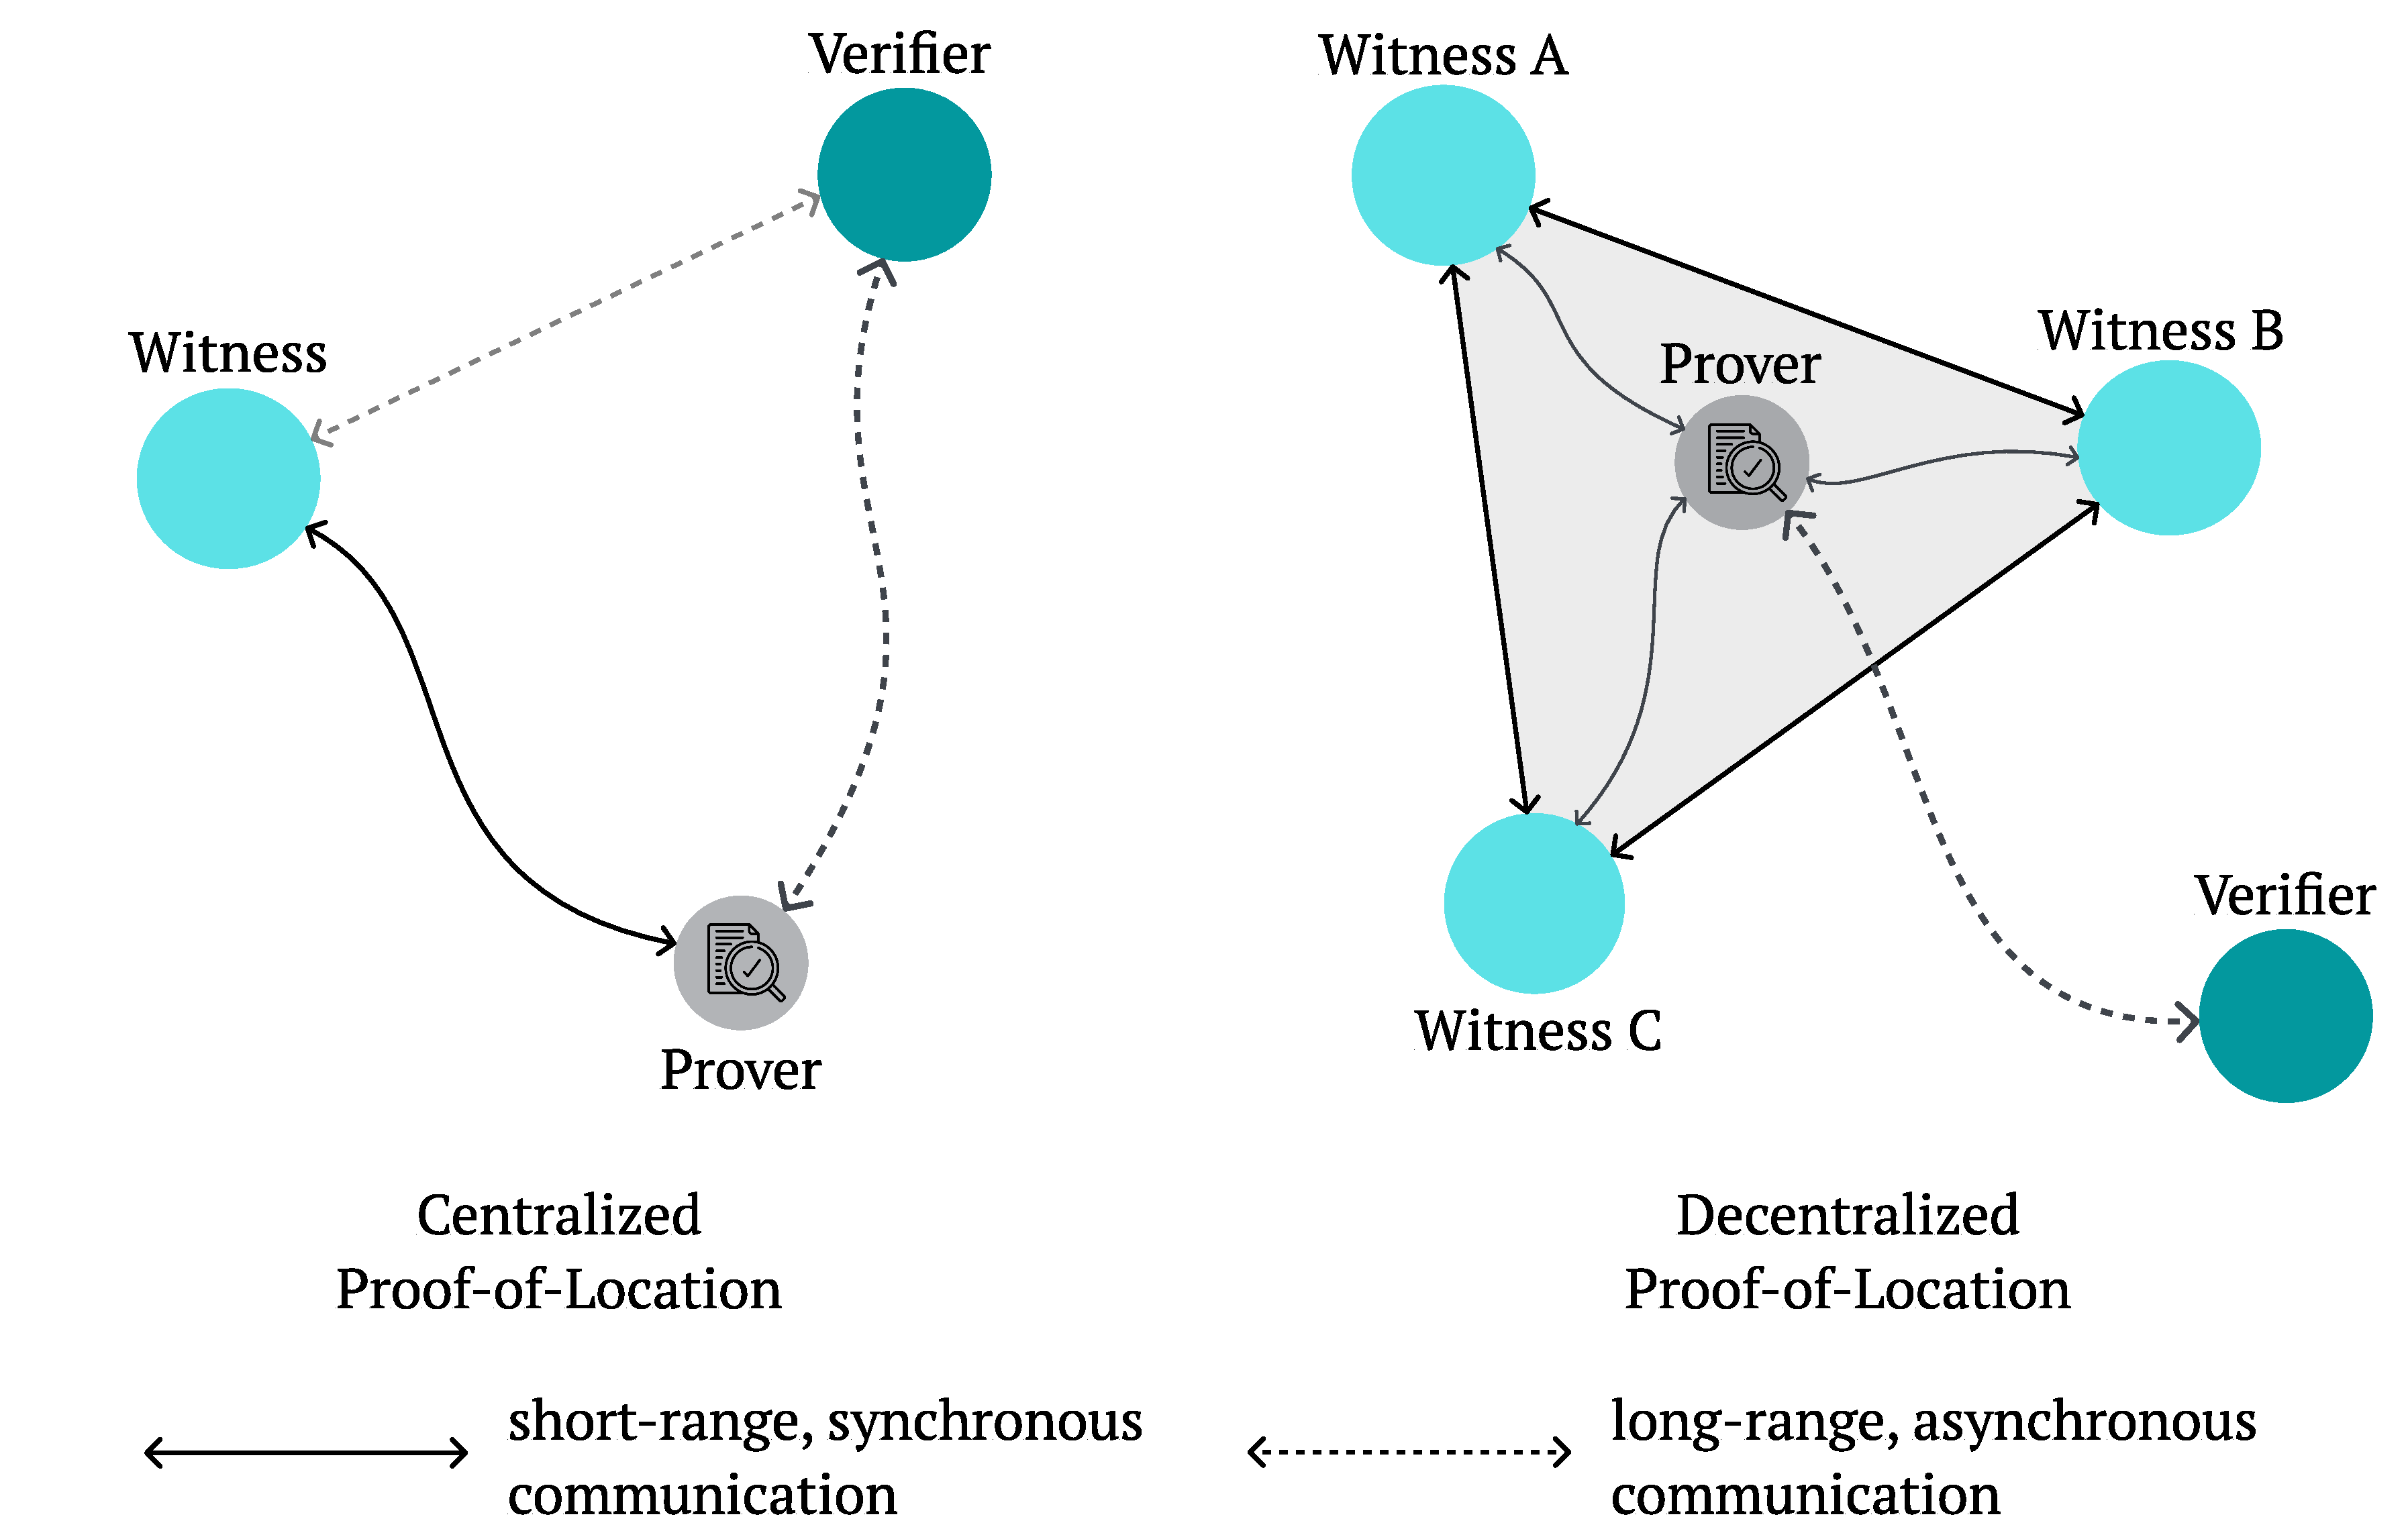
\includegraphics[width=0.9\textwidth]{proof-of-location-protocol-entities.pdf}
    \caption{The entities involved in a \pol{} protocol. The left side of the figure represents the typical arrangements of a centralized protocol, where the witness and the verifier may establish some bond between each other. The right side shows the configuration of a decentralized and trustless solution, where a quorum of witnesses attests the prover's location.}
    \label{fig:proof-of-location-protocol-entities}
    \end{center}
\end{figure}

\paragraph{Prover.} A prover is a dynamic entity, both in movement and availability terms. It is expected to be able to communicate with the witnesses, to gather a proof of its location, and to be later able to provide a location claim to the verifier. Communication with nearby witnesses is thought to happen via any short-ranged message transmission means. Provers are also expected to be associated with a verifiable but desirably private identity, often as a pseudonym.

\paragraph{Witness.} A witness is an entity that is expected to be able to communicate with the prover via the same short-ranged communication channel and to provide it with a verifiable piece of location attestation. These parties are envisioned to statically or dynamically exist around the prover's location, during the protocol process, and to maintain, in the most recent decentralized protocols, a relatively stable neighbouring list of nearby peers. Witnesses are also expected to be fictitiously identified, usually by a pseudonym.

\paragraph{Verifier.} A verifier is an external entity that is able to receive a location claim from a prover and verify its validity. Although possible and predicted for trusted setups, in a trustless environment and with the general assurances of a permissionless protocol, verifiers shall not have the need to communicate directly with the witnesses. The verifiers' identities are also of no specific importance for the protocol, since the interaction with the prover is usually asynchronous and external to the witnessing process. \\

% Chapter~\ref{sec:related-work} will describe these possible configurations in greater detail, discriminating both their infrastructural layouts and their trust assumptions.

Inspired by \cite{nasrulin2018robust, dupin2018location}, we now introduce a substantially formal but general definition of the \pol{} problem, along with some of its desirable properties:

\paragraph{Definition 1 (\pol{}).} A \pol{} is a verifiable digital certificate that attests the presence of a prover $\rho$ at location $l$ and time $t$.

\paragraph{Definition 2 (Completeness).} A \pol{} is complete if the prover $\rho$ is attested at location $l$ and time $t$, by a set of witnesses $\omega \in W$.

\paragraph{Definition 3 (Spatio-temporal Soundness).} A \pol{} is spatio-temporally sound if it is generally hard for the prover $\rho$ to obtain, forge, or modify a complete \pol{}, if not physically present at location $l$ and time $t$.

\paragraph{Definition 4 (Non-transferability).} A \pol{} is non-transferable if valid only for the prover $\rho$ that obtained it.

\paragraph{Definition 5 (Correctness).} A complete \pol{}, generated by an honest prover $\rho$, in cooperation with honest witnesses $\omega \in W$, must always be accepted by an honest verifier $\nu$.\\

Additional properties may be protocol specific, but the above definitions are generally considered to be the most common and desirable properties of a \pol{} protocol. Further formalizations can be found in the works dissected in Chapter~\ref{sec:related-work}.

\subsubsection{Common Threat Models}

Like with any technology that involves the collection and processing of sensitive and tamper-prone location data, \pol{} systems must be designed and implemented with a keen awareness of the threat landscape. The threat models of these systems are very often intricately multisided, encompassing a diverse range of actors, motives, and attack vectors. In this context, it is crucial to understand not only the technical mechanisms of \pol{} systems, but also the broader factors that shape their security and privacy risks. 

Some common scenarios that may affect the security of \pol{} systems are, for instance, malicious provers that may attempt to forge location claims, or witnesses that may attempt to collude with other entities to falsify the information. Adversary efforts may also be observed in the form of baleful provers, or witnesses, that may try to respectively impersonate other peers. Sybil attacks, which involve flooding the system with fake participants, are too on the horizon of possible threats, often employed to disrupt the operation of the protocols \cite{nasrulin2018robust}. Other works have also considered semi-honest adversaries that, despite following the protocol rules, may try to learn additional information from the messages exchanged \cite{dupin2018location}. These and other attack vectors are further dissected in Chapter~\ref{sec:related-work}, with reference to the multiple solutions that attempt at being shielded from these malicious situations.

\subsubsection{Application Scenarios}
\label{sec:background-proof-of-location-application-scenarios}

The concept of verifiable and digital \pol{} has a wide range of applications, as deconstructed by Sariou and Alec, in \cite{saroiu2009enabling}. For instance, in customer reward systems, \pol{} can be used to provide incentives to customers who visit physical stores, offering rewards and loyalty programs to verified visitors. In location-authenticated business review systems, \pol{} can be used to verify the authenticity of customer reviews. By requiring customers to verify their physical presence at the business location, businesses can prevent fake reviews and ensure that only genuine customer feedback is posted. In location-restricted web content delivery, \pol{} can be used to limit access to online content based on the user's physical location. For example, a video streaming service may use verifiable \pol{} to prevent users from accessing content outside legally allowed regions or countries. In voter's physical presence verification, a \pol{} protocol can be set to prevent voter fraud, by verifying that voters are physically present at the polling stations. Remote working and residency verification, for tax purposes, fit too in the realm of possible applications. Pournaras \cite{pournaras2020proof} goes beyond these specific cases and theorizes about an augmented democracy approach to smart city development. In the author's hypothesis, \pol{} is used to create a transparent and participatory decision-making process by enabling citizens to verify their physical presence at public meetings and events. \pol{} may also play a role in the smart mobility infrastructure, helping in verifying and optimizing the use and cost of public transportation.

Tailored to the reality that wraps the writing of this thesis, this problem becomes increasingly relevant with the advent of Artificial Intelligence (AI) tools, capable of forging highly realistic content at unprecedented scales. To combat such surge, photographers and reporters may make use of \pol{} to certify the physical originality of their photos and videos, while journalists may use it to verify the authenticity of their sources. Another use case is the verification of the provision of services, such as the delivery or supply of goods, by third-party providers. For instance, an Internet Service Provider (ISP) may use \pol{} to attest the physical deployment and provision of connectivity to a group of customers in a particular area. This can be extended to attest, as well, the quality of the service and to prevent the ISP from charging for services that are not provided, increasing overall trust and transparency. For the first use case, let's imagine a reporter who arrives at an accident site, in a busy city centre. The reporter takes out his camera and captures photos and videos of the crash. As he records, several bystanders notice and approach him. Since they all simultaneously witness the reporter's presence at the accident site, they are able to attest his physical presence at the location and time of the event, certifying the authenticity of the content that would feature later in the news. In the second use case, a group of customers has been waiting for their ISP to provide connectivity to their neighbourhood. The regulators demanded proof of the ISP's service provision, after it claimed to have provided the necessary infrastructure. To generate such proof, customers are asked to coordinate their efforts and attest the service in their neighbourhood. They all synchronously connect their devices to the infrastructure and attest the ISP's connectivity, proving it met the expected standards. They all proceed to sign the attestation and submit the proof to the regulatory authorities. These two examples are depicted in Figure~\ref{fig:proof-of-location-example-scenarios} and will feature in the following chapters, bridging the specification of the \pol{} protocol with real world use cases.

\begin{figure}[h!]
    \begin{center}
    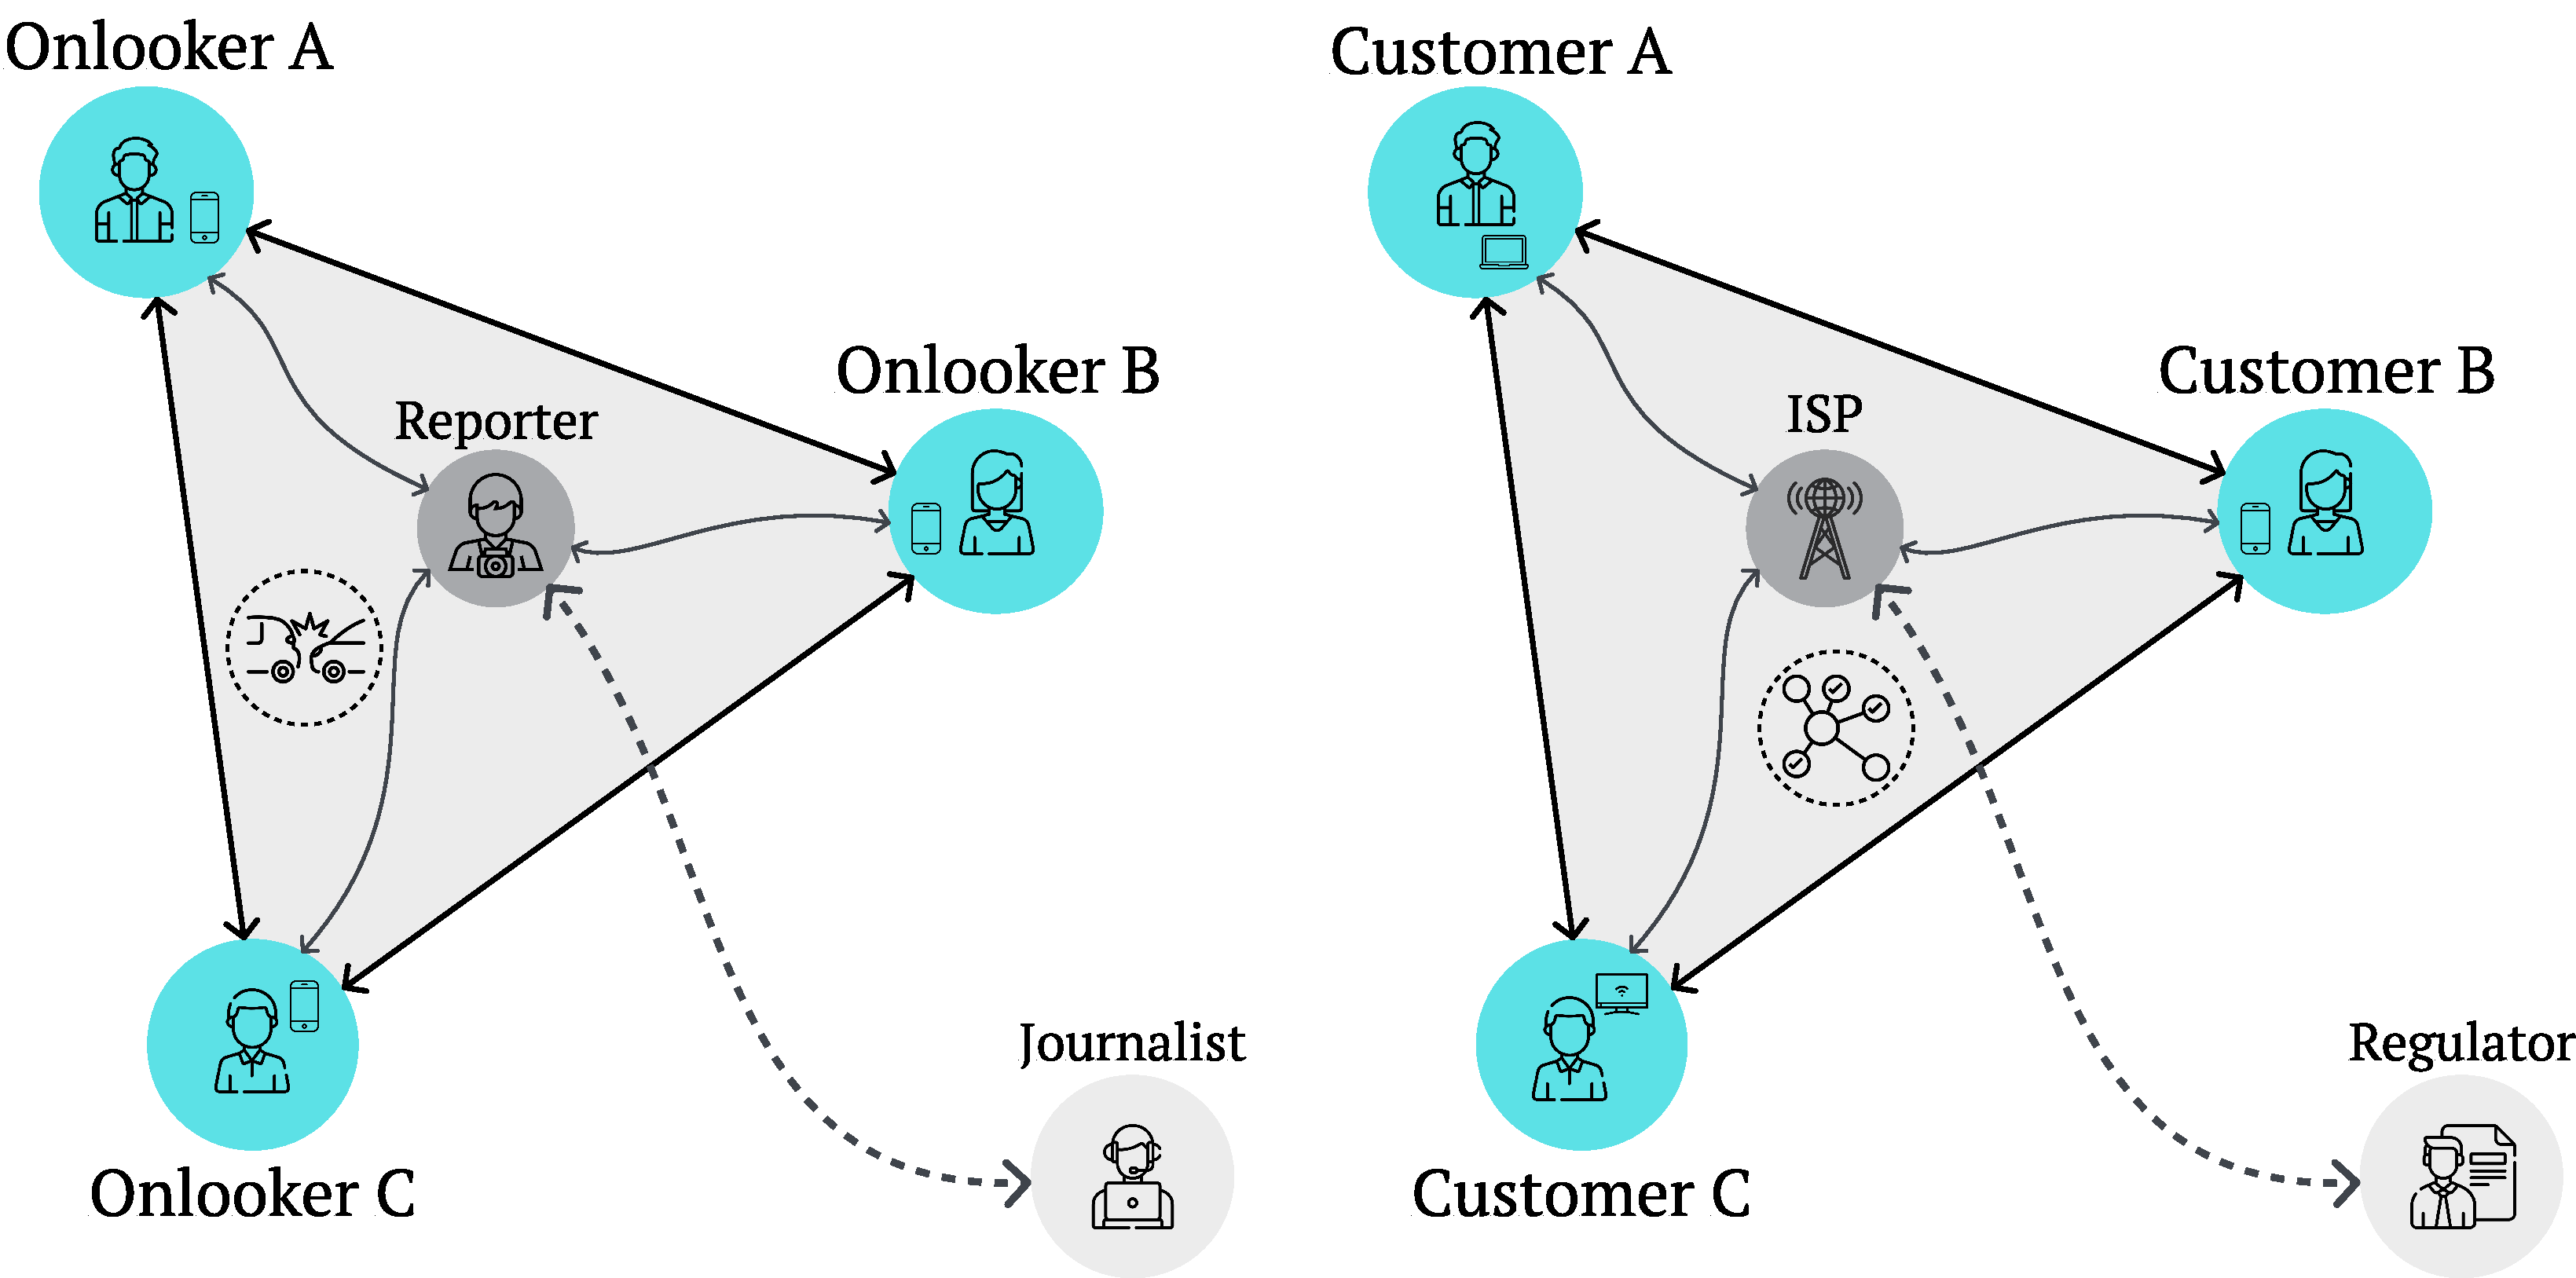
\includegraphics[width=0.8\textwidth]{pol-examples.pdf}
    \caption{Examples of \pol{} applications.}
    \vspace{-0.5cm}
    \label{fig:proof-of-location-example-scenarios}
    \end{center}
\end{figure}

Targeting different trust levels, additional application scenarios can be derived from the above, while many others are yet to be discovered. Given all this, digital and verifiable \pol{} has a wide range of applications that may disruptively benefit individuals, businesses, and the society as a whole. Chapter~\ref{sec:related-work}, afterwards, gives a more nuanced overview of both the evolution of the protocols and specific use cases that these multiple solutions aim at covering. The next section will introduce the technologies that are set to enable short-range communication between the entities of a \pol{} protocol.

\subsection{Mesh Networks} \label{sec:background-wireless-mesh-networks}

The envisioned fourth industrial revolution has set the track for modern advancements in achieving a global web of pervasive connectivity between all sorts of machines \cite{akyildiz2005wireless, cilfone2019wireless}. New means of radio and wireless communication have been pushing for the technological heterogeneity of protocols, architectures, devices, and consequent performance levels, in order to find their design suitability for different coverage or range scenarios, transmission or bandwidth rates \cite{sichitiu2005wireless}. Additionally, requirements for more complex, adaptable, and resilient topologies have captured broad interest, in both academic and industry domains. 

The development of new hardware, protocols, and applications started gaining momentum and branched their way forward to support the popularisation of Wireless Mesh Networks (WMNs). In mesh topologies (see Figure~\ref{fig:mesh-network-topology}), network nodes are directly and dynamically connected in a non-hierarchical way. This trait eventually allows for many-to-many communications between the devices, to efficiently route data from a generic source to a generic destination. The infrastructure nodes that make up the mesh are expected to dynamically self-organize and configure themselves, resulting in beneficial distributed effects on the overall fault tolerance, ease of deployment, and workload allocation \cite{cilfone2019wireless, sichitiu2005wireless}. WMNs follow these principles with the particularity of being made up of radio nodes that communicate via any sort of wireless means.

\begin{figure} [h!]
  \begin{center}
  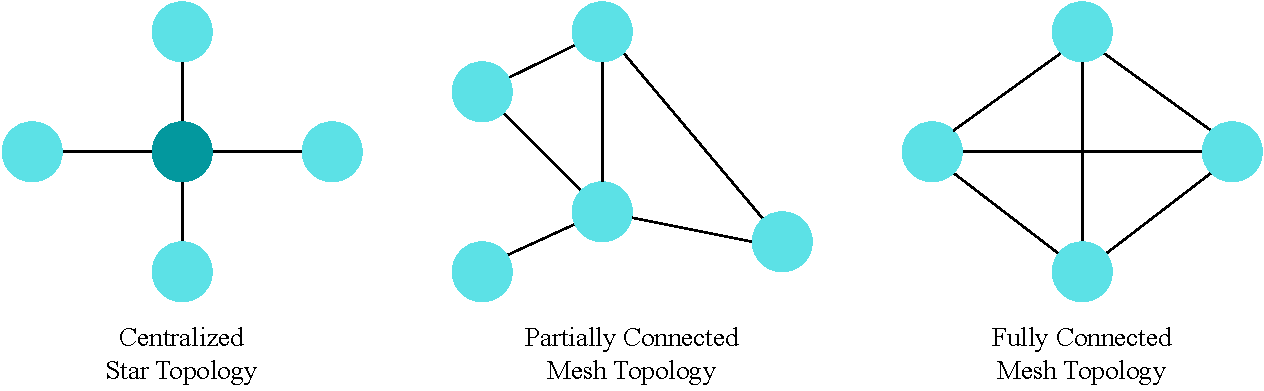
\includegraphics[width=0.8\textwidth]{network-topologies.pdf}
  \caption{Examples of different topologies of a computer network. Starting on the left, the star topology shows all the nodes connected to a central hub. To the right, examples of mesh topologies depict the direct and decentralized connections between the nodes.}
  \label{fig:mesh-network-topology}
  \end{center}
\end{figure}

Some of the most common technologies that have been, throughout the years, ported to WMNs are Bluetooth, LoRa and IEEE 802.11. The first two are prominent solutions for the extremities of the mesh networking spectrum, with Bluetooth under the short-range realm of Personal Area Networks (PANs), and LoRa  under the Low Power, Wide Area (LPWA) scenario. Downsides of these technologies are, respectively, the limiting coverage range for one-hop neighborhoods, or the low bandwidth rates \cite{cilfone2019wireless}. Hence, IEEE 802.11 became the most flexible and widely used technology, being the basis of the Wi-Fi standard, which, at the beginning of the last decade, saw an amendment that mainly targeted mesh networks~\textemdash~the IEEE 802.11s WLAN Mesh Standard \cite{hiertz2010ieee}. The novelty came with the introduction of routing mechanisms operating at the ISO/OSI Layer 2, allowing for compatible information delivery in the layers above. The dynamic establishment of a topology for IEEE 802.11s-based mesh networks relies on the phased transmission of beacon messages that allow for the discovery, synchronization, and maintenance of the links between the peers. IEEE 802.11s has a default routing protocol, the Hybrid Wireless Mesh Protocol (HWMP), which is based on a series of flooding procedures for both proactive and reactive path finding and selection \cite{bari2012performance}. However, this protocol is not strictly enforced by the standard and has been replaced by other more popular solutions. One notable example is the Better Approach To Mobile Ad-hoc Networks (B.A.T.M.A.N.) routing protocol.

This thesis will explore the concept of mesh networks and their potential for serving as the infrastructural topology that enables the relatively short-ranged exchange of messages between the participants of a \pol{} protocol. The following sections will present the B.A.T.M.A.N. routing protocol, OpenWrt, and other relevant tools that will be later used to implement the \poc{}.

\subsubsection{B.A.T.M.A.N. Routing Protocol}

The Better Approach To Mobile Ad-hoc Networks (B.A.T.M.A.N.)\footnote{\url{http://www.open-mesh.org/}} is a proactive routing protocol for WMNs, operating at the data link layer instead of the network layer, asserting the reliability of radio links using routing metrics and a distance-vector approach \cite{seither2011routing}. Its newer version, \emph{batman-adv}, has gained traction and popularity and eventually made itself available in the Linux kernel.

Route discovery is preemptively replaced with neighbour discovery, and each infrastructural node is instructed to calculate its potential best next-hop, significantly reducing the overhead of requiring each peer to be aware of the whole network topology. Its version V introduced a throughput metric to evaluate the links' quality and routing choices, replacing version IV packet-loss metric, deemed unsuitable for larger network sizes \cite{seither2011routing}.

\begin{figure} [ht]
  \begin{center}
  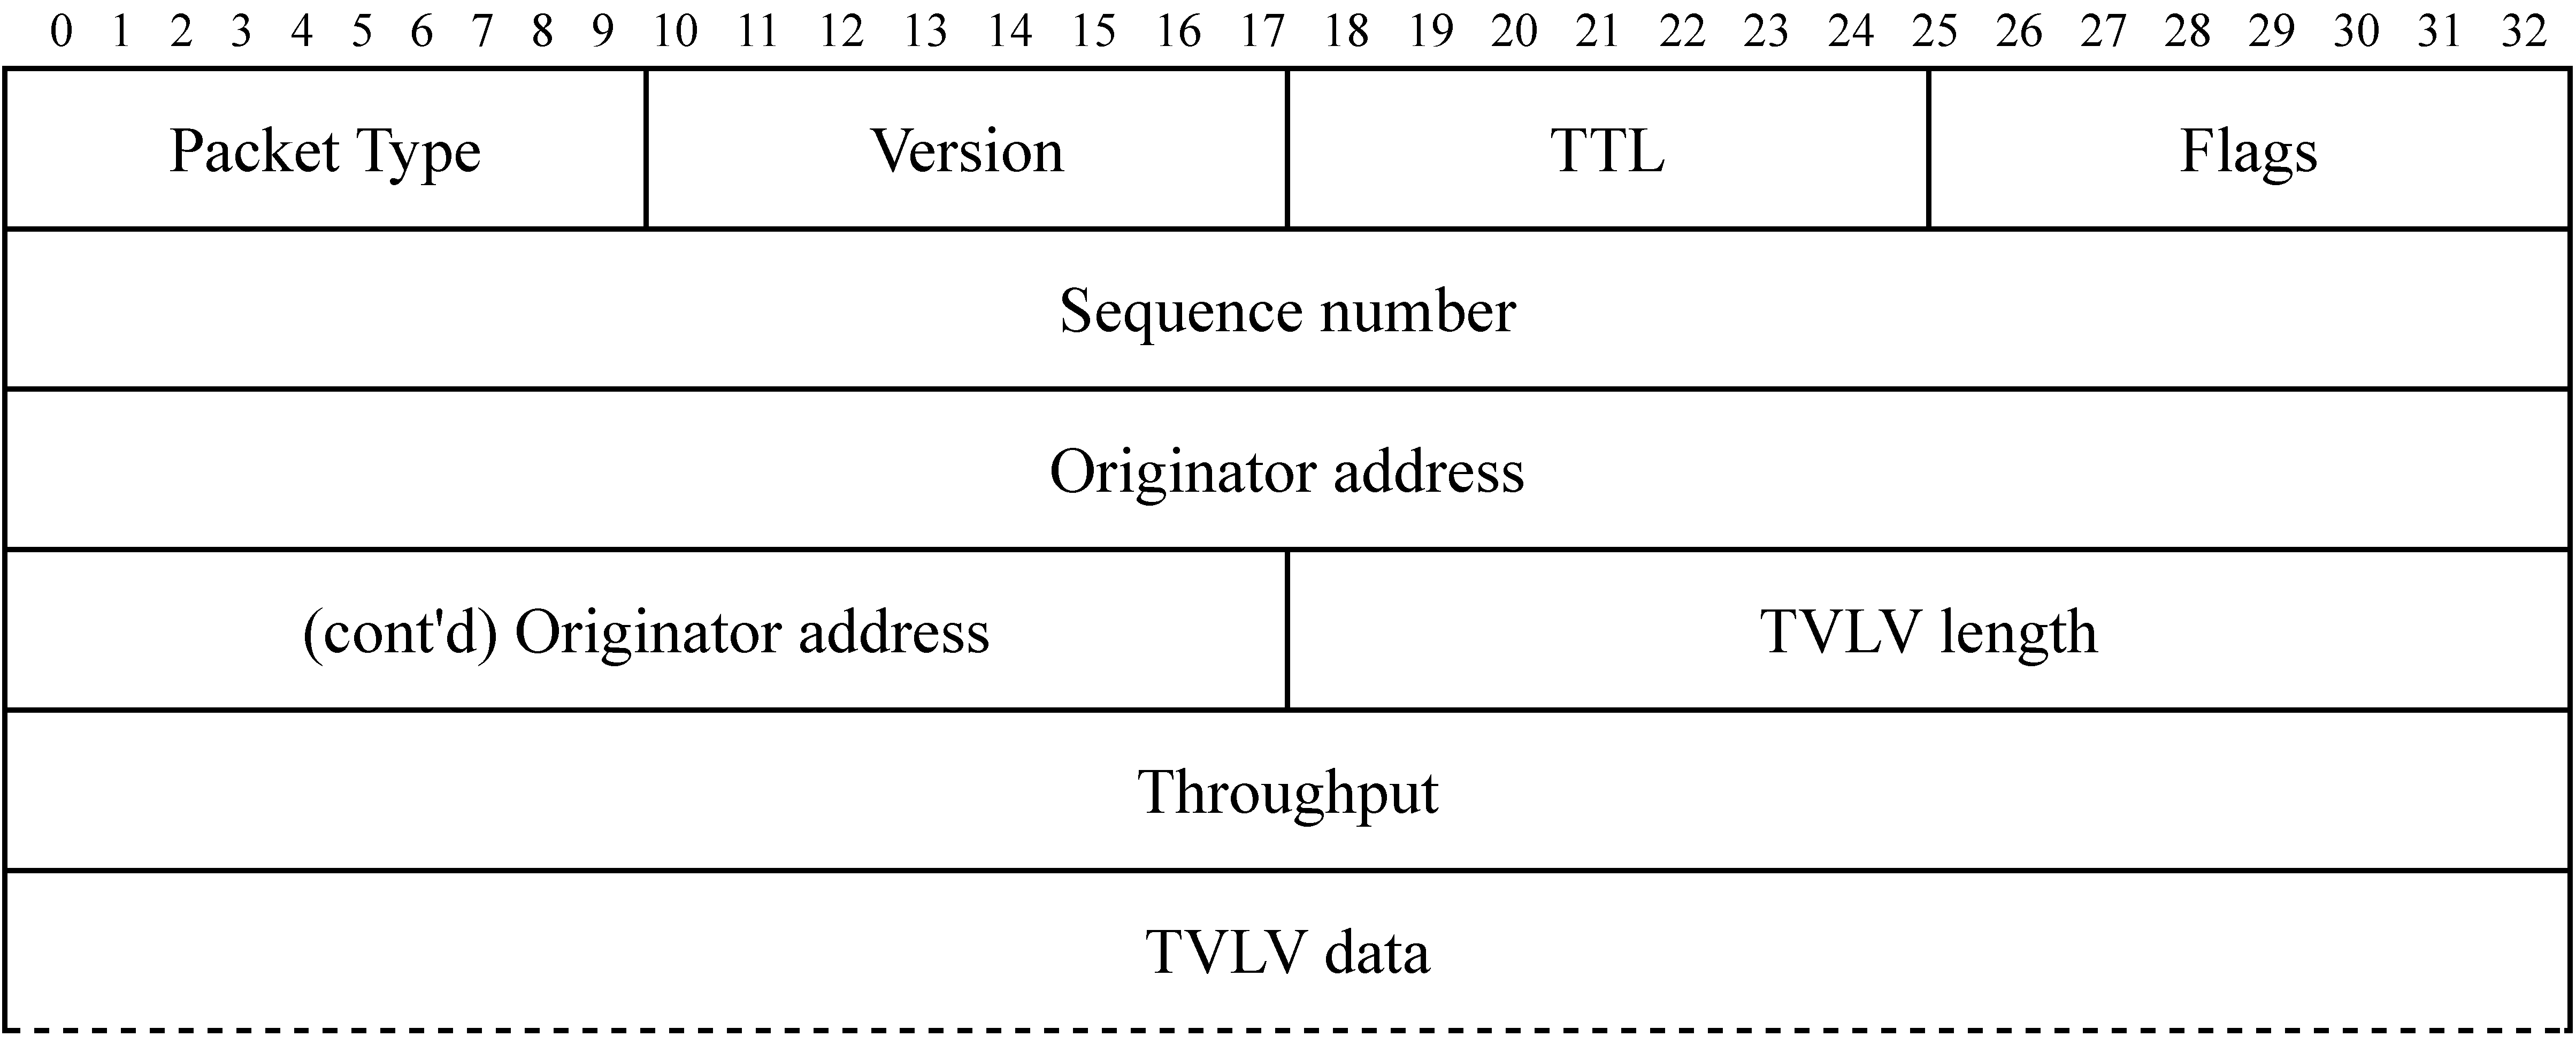
\includegraphics[width=0.9\textwidth]{batman-adv-ogmv2.pdf}
  \caption{OriGinator Message version 2 (OGMv2) packet format \cite{cilfone2019wireless,open-mesh-ogmv2}. These messages are broadcasted with a collision avoidance delay mechanism defaulting to 1 second. The packets contain, among other fields, the originator's MAC address and throughput metric values, measured in units of 100 kbit/s.}
  \label{fig:batman-adv-ogmv2}
  \end{center}
\end{figure}

The discovery of neighbouring nodes is accomplished with the capture of broadcasted OriGinator Messages (OGMv2, see Figure~\ref{fig:batman-adv-ogmv2}), that feature a collision avoidance delay mechanism, the detection of new or duplicate messages, and other fields for throughput measurement and gateway discovery. The Echo Location Protocol (ELP) handles the received messages and ranks the discovered neighbours. The OGM flooding protocol, on the other hand, enables mesh routing procedures that, simultaneously but independently, allow for estimating the quality of the individual links \cite{cilfone2019wireless}. Additionally, the protocol facilitates OGM aggregations as an effort to reduce the overhead of sending many short-sized frames. Nevertheless, there is still a quest for optimizations that would allow for more efficient use of multiple interfaces. An implementation of a subset of the Internet Control Message Protocol (ICMP) is also made available, allowing, for instance, the use of the \emph{ping} command to test the connectivity between nodes \cite{seither2011routing}.

Building on the previous, the B.A.T.M.A.N. routing protocol has been, through multiple initiatives, successfully blended into the OpenWrt project, which will also be employed in the \poc{}. The following section will present OpenWrt and other relatable tools.

\subsubsection{OpenWrt, QEMU, and Raspberry Pis}

The OpenWrt project\footnote{\url{https://openwrt.org/}} is a Linux distribution for embedded devices, which, in the context of this thesis, will serve as the host operating system for running the \poc{} solution. The project is based on the Linux kernel, encapsulating several of its libraries and packages, and is designed to be used on resource-constrained devices. OpenWrt features not only a writable root filesystem and automated build tools with integrated cross-compiler toolchain, but also a package management system that allows for the installation of additional software. The project also provides extensive configuration options for networking capabilities, which includes enabling mesh networking support through the B.A.T.M.A.N. routing protocol. 

To facilitate the development and testing of the \poc{}, the QEMU\footnote{\url{https://www.qemu.org/}} emulator will be used. QEMU is a generic and open-source machine virtualizer that, through its versatile set of features, allows for the full-system emulation of a wide range of hardware and software. The emulator will run the OpenWrt generated images and spawn multiple virtual machines. These machines will simulate the various protocol participants by establishing, with the help of the network emulation tools, a fully connected mesh network. The intention is to ease and accelerate the development process by allowing for testing the \poc{} in a controlled environment, without the management, maintenance, and deployment hustle of physical devices. Later, the solution is planned to be deployed on a set of Raspberry Pis\footnote{\url{https://www.raspberrypi.org/}}, the most widely used single-board computers for developing IoT solutions. The implementation journey will be documented in Chapter~\ref{sec:proof-of-concept}.


\subsection{Permissionless Consensus} \label{sec:background-permissionless-consensus}

% The following section and subsections reuse the work done in the Distributed Systems Seminar, during the fall semester of the 2022/2023 academic year. The original version of the seminar paper can be found in \cite{units-of-permissionless-consensus}.

Long has been the time when consensus was still on the verge of being considered such a fundamental problem of distributed systems. Generally defined by Lamport et al. \cite{pease1980reaching, lamport2019byzantine}, consensus means reaching an agreement between multiple parties in the potential presence of faulty individuals. As per multi-agent systems, interacting over computer networks, consensus is thought to be the result of a coordination effort, that eventually leads the parties to agree on some value at a given moment. However, the evolution of the consensus problem has been invariably limited by a set of strong assumptions. The well-known Byzantine-Fault-Tolerant multiparty consensus systems, that have been designed over the years, are usually meant to work only with a set of known participants, being them faulty or not \cite{castro1999practical}. 

The other side of the coin is the permissionless consensus challenge, consisting of achieving agreement in an environment where the parties are unknown and untrusted \cite{nakamoto2008bitcoin, buterin2014next}. The relative openness and lack of any kind of central authority are other intrinsic particularities of this type of networks, which inevitably adds complexity to the problem. The participants are not only unknown and untrusted but can also join or leave the network at any time, freely choosing if they care to participate in the consensus protocol. Nevertheless, the problem of permissionless consensus is still seen as a special case of the general consensus definition, but under more meticulous trust assumptions.

Further in this thesis, we will evaluate the different high-level \pol{} protocols and draw a parallel between the evolution of their trust levels and the ultimate need for a low-level permissionless consensus algorithm that allows for establishing decentralized and time-conscious agreement, in an eventual trustless setup, between the multiple witnesses. The next subsections will briefly review some of the most relevant aspects and proof units that give practicality to the roots of the permissionless consensus problem.

\subsubsection{Proof-of-X}

The solution is, nonetheless, unsettled and the scientific community has been reasoning about the need for permissionless consensus when there are already well known and established consensus protocols that work in trusted environments \cite{castro1999practical, miller2016honey}. However, even those protocols have their own limitations, not only in terms of trust, fault-tolerance, centrality, permissions, or bottlenecks, but also in terms of scalability \cite{miller2016honey}, despite assuring deterministic finality \cite{decker2016bitcoin}. The need for permissionless consensus is then justified by the fact that permissioned protocols are not compatible with the requirements of the new generation of distributed systems, especially in the context of Blockchain networks. These requirements include dealing with today's sparse networks of anonymously and dynamically participating devices, without interrupting consensus and while battling the disruption of the system, typically by subverting it with many pseudo-entities~\textemdash~the so-called Sybil attacks \cite{8629877, survey-dist-consensus}. Fundamentally, the permissionless consensus problem is the need for a consensus protocol that can be run in a distributed and decentralized environment, where the participants are unknown and untrusted, and where the network is bigger, sparser and unpredictably less reliable.

Technically, permissionless environments allow for larger networks that depict lower connectivity between the participants. Operationally, everything is expected to happen in an asynchronous or partially synchronous fashion, and the number of transactions is predicted to be smaller than in the permissioned counterparts. Participation is free, and the governance is not centralized, but rather distributed and public. The identity of the participants is secured or semi-secured as it often relies on pseudonymity for protecting the nodes' identity, enabling, at the same time, full transparency concerning the rest of the network's content and operation \cite{xiao2019distributed}. Expectedly, the goal of permissionless consensus, as for any consensus protocol, is to reach agreement on a single value, or a set of values. However, due to the nature of the protocols, the values that are agreed upon end up establishing the serialization of the transactions, and so establishing time consciousness and total order of the events \cite{8629877}.

Also described by Xiao et al. \cite{survey-dist-consensus}, very concisely, the way to achieve an operating protocol, as seen in the mainstream blockchain networks, is by first generating the agreeable value, in this particular case, a block and its proof. Next is the phase of proposing and disseminating the information to the network, followed by the eventual validation and acceptance of the block by the majority of the nodes. This is the approximate moment of probabilistic finality, when consensus is ultimately reached (see Figure~\ref{fig:building-blocks-consensus}). During the whole process, a fair and somewhat predictable incentive mechanism is also needed, that rewards participants for their honest effort in reaching consensus, and punishes the ones that are not behaving correctly. These incentives are of major importance in this very context of permissionless consensus, and all these building phases form the basis of the inner functioning of Bitcoin itself \cite{nakamoto2008bitcoin}, replicated with some variations in other networks \cite{buterin2014next, survey-dist-consensus}. The following section is a short introduction to some relevant proof units that feature in the most popular blockchain systems.

\begin{figure}[h!]
  \begin{center}
  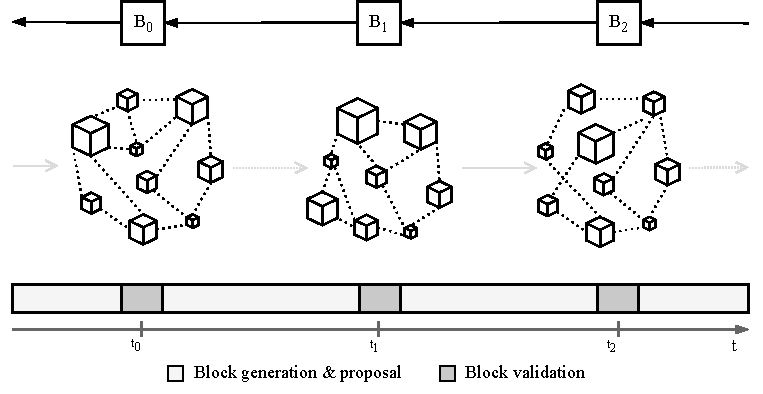
\includegraphics[width=0.9\textwidth]{building-blocks-consensus.pdf}
  \caption{An illustration of the permissionless consensus building phases. From the bottom to the top, the asymmetric arrow of time discretizes the block generation and proposal phases, followed by the block validation, along with frequent network topology changes and the consequent time conscious serialization of the blocks.}
  \label{fig:building-blocks-consensus}
  \end{center}
\end{figure}

\subsubsection{Proof-of-Work and Proof-of-Stake}

Without discrediting the previous attempts, the first practical permissionless consensus algorithm was proposed by Nakamoto in \cite{nakamoto2008bitcoin}. It is a Proof-of-Work consensus protocol that resembles a replicated state machine where the independent participants reach agreement not only about transactional values, but also about their order~\textemdash~naturally forming the underlying structure of what is now known as a blockchain. The focus shifted for decentralized systems and after Proof-of-Work many other consensus mechanisms have been proposed, relying on different consensus units.

In the classical Nakamoto consensus protocol, the generation of a block, to be proposed for further network agreement, complies with the unit of computational work needed to create, or rather find, a verifiable proof of the effort spent on assembling the block \cite{nakamoto2008bitcoin}. This essentially requires brute forcing the search for a cryptographic hash value for the aggregation of the block information with a nonce. This value has to satisfy a difficulty threshold (see Procedure \ref{proc:BlockGeneration}), which gets adjusted dynamically over time, to maintain the network overall requirement for the block generation interval \cite{8629877, survey-dist-consensus}.

\begin{procedure} [!h]
	\caption{BlockGeneration()} \label{proc:BlockGeneration}
	\KwIn{Transaction Merkel Tree Root, Hash of the last Block, Timestamp, Other.}
	\KwResult{new $Block$.}
	\BlankLine
  $BlockHeader \ \gets$ Transaction Merkle Tree Root
  \\ \qquad $| \ $ Hash of the last Block
  \\ \qquad $| \ $ Timestamp
  \\ \qquad $| \ $ Other\;
  \BlankLine
  \tcp{the preceding zero bits in $target$ depict the mining difficulty}
  \While{$Hash(BlockHeader \ | \ nonce) \geq target$}{
    Increment $nonce$\;
  }
  \tcp{append transactional data}
  \Return new $Block$\;
	%\eIf{error messages were found}{\Return \False\;}{\Return \True\;}
\end{procedure}

One can then exercise the reasoning line and extrapolate the previous block generation mechanism to a \emph{Proof-of-Something} pseudo-random competition in which an entity in possession of a higher amount of a certain resource, either computational power, or stake, or certain currency, or, for instance, a higher amount of storage space, guarantees a higher probability of leading the block generation and proposal, consequently winning the acceptance by the majority. This is the essence of Proof-of-Stake, as a derivative of the Proof-of-Work mechanism. Here, stake is a traceable and verifiable amount of a certain unit, token or currency, that is owned by a certain entity who wishes to participate in the consensus protocol. The stake works as a form of collateral that is used to guarantee everyone's honesty, in an attempt to reduce the Sybil attack likelihood. And, respectively as in Proof-of-Work with computational power, the higher the stake, the higher the probability of leading the block generation and proposal.

Idealized and inspired by Proof-of-Stake, extending or adapting Proof-of-Work became a popular trend in the blockchain community. The main idea is to replace the computational power with some other resource, that is more scarce, or more valuable, or more verifiable, or more traceable, to combine multiple resources, or even to add extra requirements to pure Proof-of-Work \cite{survey-dist-consensus}. Not that every one of the options has a considerable potential for entirely solving the permissionless consensus problem, but each one of them may tackle different use cases where consensus needs to be reached, and where different resources are available to make the agreement happen \cite{BOURAGA2021114384, 9376868}. Nonetheless, the design of these consensus mechanisms shall aim for a protocolar choice between a set of properties that form a trilemma: security, scalability, and decentralization. Briefly put, relaxing the security requirements may allow for more scalability, both of which, consequently, have hands tied with decentralization. These trade-offs are of practical consideration when defining the network goals and use cases \cite{survey-dist-consensus}. Further dissection of various classes of Proof-of-Stake based protocols, diverging alternatives to the classic Nakamoto consensus, and comparisons between them can be found in \cite{8629877, survey-dist-consensus, BOURAGA2021114384, 9376868, natoli2019deconstructing}.

With all the above in mind, we will proceed to review some of the proposed \pol{} solutions, discriminated by trust levels. Aiming at achieving spatio-temporal agreement among the witnesses, we will reason about the applicability of one of these permissionless consensus protocols, in the context of a fully decentralized and trustless environment.

\newpage
\section{Related Work} \label{sec:related-work}

This chapter presents a description of the current state of the \pol{} problem, spanning the spectrum of its trust levels, from fully trusted to permissionless environments. Furthermore, it encompasses an assessment of the typical infrastructural scenarios, detailing the progressive shift from centralized to decentralized systems. The organization of the chapter is as follows. Section~\ref{sec:related-work-trusted-centralized} outlines the starting point in a trusted and centralized setting. Section~\ref{sec:related-work-distributed-decentralized} details the progressive shift towards distributed and decentralized protocols. Finally, Section~\ref{sec:related-work-fully-trustless} presents the most recent developments in the \pol{} problem, which ultimately target permissionless and fully trustless setups. 

% Finally, alternative strategies to the prevailing \pol{} protocols, which this thesis mainly addresses, are presented in Section~\ref{sec:related-work-alternative-strategies}.


\subsection{Trusted and Centralized Architectures} \label{sec:related-work-trusted-centralized}

The establishment of not just the concept, but also the need for a new kind of systems that, in simple terms, would allow for attesting and prove some device's location, dates back to the early beginnings of this century. 

Waters and Felten, in \cite{waters2003secure}, attempt at pioneering the design of a location-proving system by proximity that simultaneously ensures integrity and privacy. The system model assumes a fully trusted setup, fundamentally composed by two entities, a \emph{verifier} and a \emph{device}. The latter is implicitly thought to be managed by an untrusted \emph{user}, but hypothesised and expected to be tamper-resistant, and thus, trusted by the verifier. The motivation behind this scenario is oriented towards practical situations in which, for instance, trusted parties lend their equipment to users and want to verify, or monitor, the equipment's location, such that it remains inside some pre-established location boundaries. The authors explicitly mention the lending of computers by universities and the wish that those devices do not leave the campuses. Home arrest monitoring systems have, as well, the need for ensuring that the ankle device, and so the person in charge, does not escape a certain location. 

\begin{figure}[ht]
    \begin{center}
    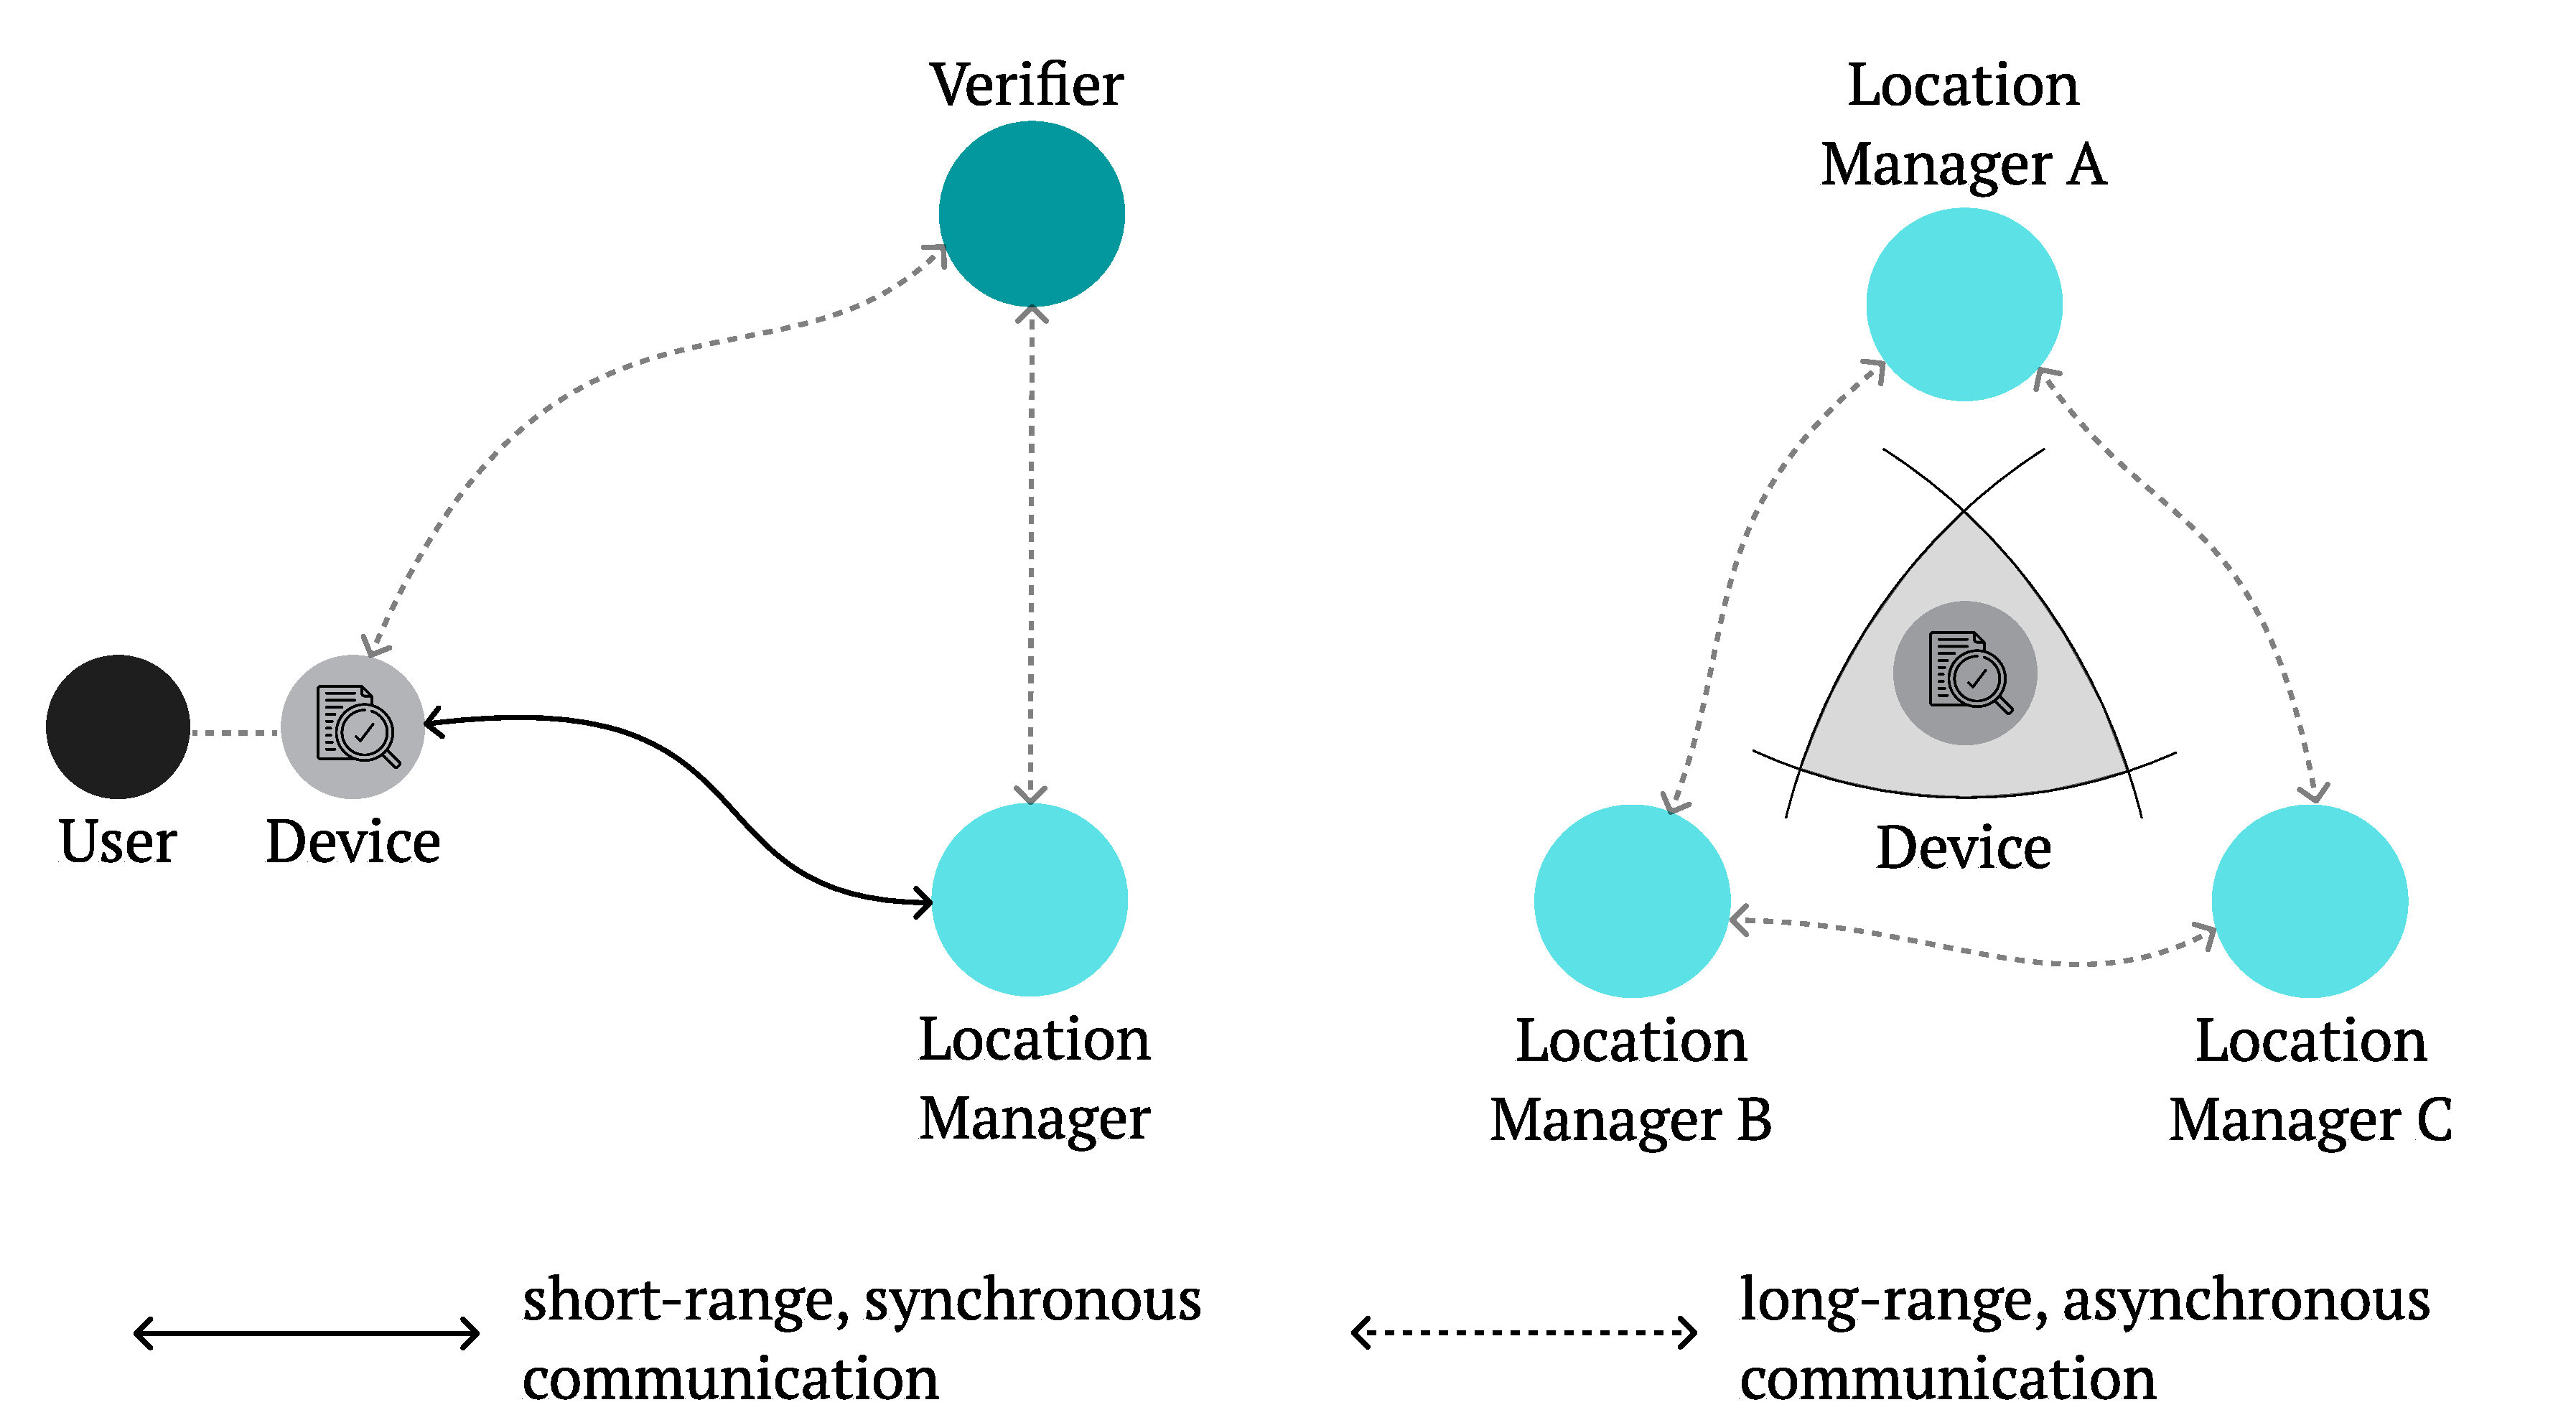
\includegraphics[width=0.9\textwidth]{trusted-centralized-pol.pdf}
    \caption{Waters and Felten's trusted and centralized \pol{} system \cite{waters2003secure}.}
    \label{fig:trusted-centralized-pol}
    \end{center}
\end{figure}

Faced with the design and coverage unadaptability of GPS-based location systems, which do not structurally aim at serving as \pol{} enablers, the authors identify the need for small wireless networks, covering a relatively short-ranged area, via a \emph{location manager} that acts as an access point. Figure~\ref{fig:trusted-centralized-pol} illustrates the multiple entities of the protocol. The device is set to accept input from an untrusted source, the user, containing the identity of a nearby location manager. After receiving this input, the device will try to prove it is physically close to the designated location manager. Aiming at a more secure and precise positioning system, the device may conduct three simultaneous proofs of proximity with three location managers, to determine its relative location. These location managers are either distinctively trusted, or set up by the verifier \cite{waters2003secure}. Round-trip and signal propagation latency are the metrics used, respectively, for determining the proximity of the device to the location manager and for protecting against proxy attacks~\textemdash~when a proxy device is placed near the location manager and serves as signal repeater for the original device that is somewhere else, outside the coverage area. The work targets Wireless LAN network operators and their existing access points' infrastructure to serve as location managers. A Public Key Infrastructure (PKI) is also proposed in order to delegate the atomic responsibility of authenticating and managing their identities to a trusted third party. Finally, the authors set down the seeds for extending their proximity proof system to a secure and moderately accurate positioning proof mechanism, with the possibility of using multiple location managers and a triangulation algorithm.

Waters and Felten's work pioneered the development of \pol{} systems, marking the first steps towards more comprehensive definitions of location proofs. Sariou and Alec, in \cite{saroiu2009enabling}, concisely introduce the primitive concepts around \pol{} and some desired properties of an inherently secure system. However, the key contribution of their work was the delineation of a set of example applications that would benefit from \pol{} protocols. These include, but are not limited to, customer reward systems for physical stores, location-authenticated business review systems, location-restricted web content delivery, voter's physical presence verification, among many others. For a more thorough depiction of such application scenarios, see Section~\ref{sec:background-proof-of-location-application-scenarios}.

Further protocols took inspiration from this groundwork and started shaping the landscape. Graham and Gray, in \cite{graham2009protecting}, propose a \pol{} scheme called SLVPGP that removes the need for the location manager to be trusted by the central verifier, delegating the trust to tamper-resistant modules. VeriPlace, by Luo and Hengartner \cite{luo2010veriplace}, is a complex and expensive privacy-aware location proof architecture that distributes responsibility among three types of trusted entities, taking the first step at avoiding dedicated tamper-resistant hardware. It specifically targeted the integration with Yelp\footnote{\url{https://www.yelp.com}}, a public crowd-sourced reviews system for businesses. Another piece worth mentioning is from Javali et al. \cite{javali2016alice}, still in a centralized and trusted stand, that adds robustness to the previous protocols by simplifying, in theoretical and practical terms, with trusted and existing Wi-Fi infrastructure, the \pol{} generation process. Finally, the work of Akand et al. \cite{akand2021privacy} is a more recent solidification attempt in the design of centralized but provably secure \pol{} systems that protect against geo-tampering attacks.

The next section will report the emergence of the first relatively distributed \pol{} protocols, taking a step further in the direction of fully decentralized and trustless systems.

\subsection{Progressively Distributed and Decentralized Protocols} \label{sec:related-work-distributed-decentralized}

VeriPlace had already profiled and templated an inherently distributed architecture with built-in privacy awareness, taking a first infrastructural step towards defending against proxy attacks, without the need for trusted hardware \cite{luo2010veriplace}. The whole setup is especially tangled and consequently resourceful for the levels of trust it assumes, but it definitely settled the ground for the next generation of \pol{} schemes. 

\begin{figure}[ht]
    \begin{center}
    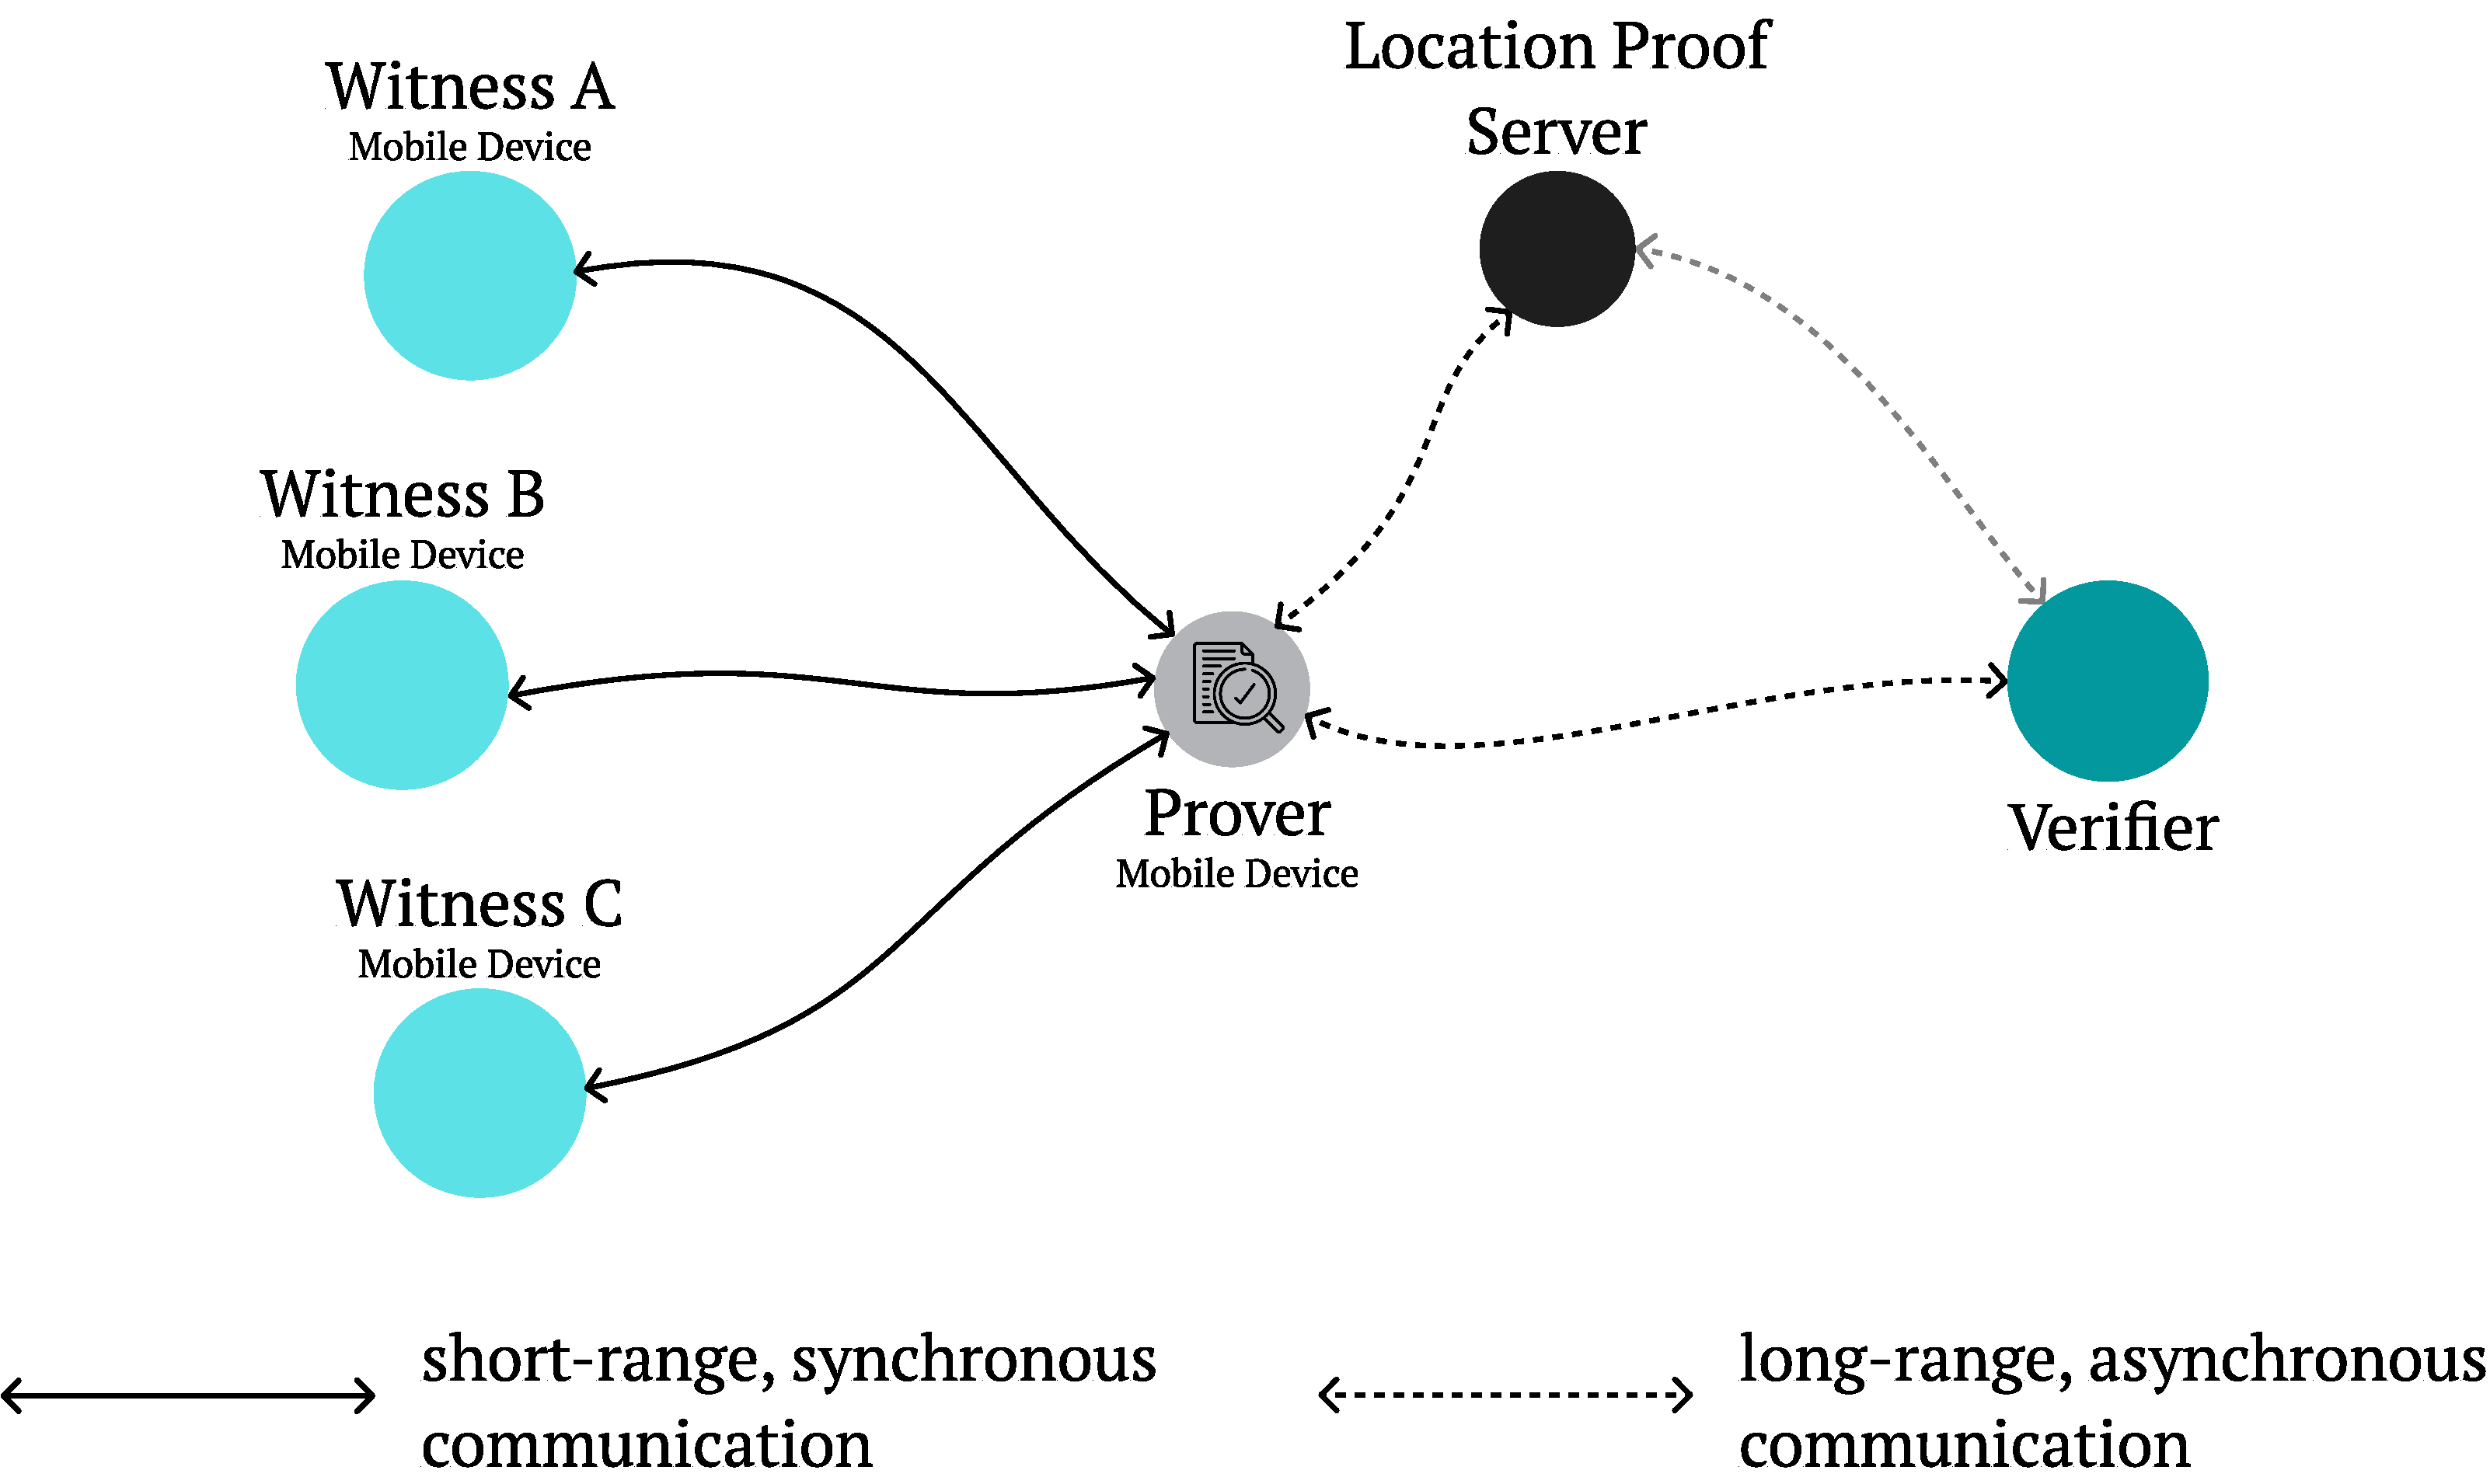
\includegraphics[width=0.9\textwidth]{decentralized-pol.pdf}
    \caption{The main arrangements of the APPLAUS protocol, by Zhu and Cao \cite{zhu2011applaus}.}
    \label{fig:decentralized-pol}
    \end{center}
\end{figure}

The following evolutionary stage of these protocols aims at flexing and distributing trust, resources, power, and responsibility, with the hope of achieving more resilient, fault-tolerant, and scalable systems. APPLAUS, by Zhu and Cao \cite{zhu2011applaus}, delivers one of the first distributed protocols that combines the location proof and location privacy problems. It uses Bluetooth enabled mobile devices that communicate with nearby participants, during the proof generation process. The protocol asserts certain bond levels between the \emph{prover}, \emph{verifier}, and \emph{witnesses}, all of them known to a trusted Certificate Authority (CA), disregarding, on the other hand, the need for a fully trusted location proof server to store the historic location records. In Figure~\ref{fig:decentralized-pol}, the essential configuration of the protocol is displayed, envisioning the prover to communicate individually, via Bluetooth, with nearby witnesses. Each witness should agree on providing a location proof, upon the prover's request, to be submitted later to an untrusted location proof server. This server will store the location proof historic records, to be queried by the verifier, in order to assert a prover's location within a specific time period. The prover, witnesses, and verifier are all assumed to be trusted by each other, leaving out the location server. The claim is that, by statistically changing the pseudonyms for each device and by following a user-centric privacy model, the protocol can effectively generate privacy preserving location proofs and store them in a trustless manner. STAMP \cite{wang2016stamp} and PROPS \cite{gambs2014props} are two contemporaneous works that take the same witnessing approach as APPLAUS, but follow the path of convincing the verifier by presenting several shares of a composite location proof, based on group signatures. Both of them try to more profoundly tackle the prover's and witnesses' privacy concerns, but may admittedly fail at preventing collusion scenarios between them. Gambs et al. argue that the reliance on a trusted third party may be an unavoidable requirement, even if against the authors' principles of location sovereignty, especially when one wants to entirely prevent unbounded collusion attacks \cite{gambs2014props}. SPARSE, by Nosouhi et al. \cite{nosouhi2018sparse}, avoids the typical distance-bounding mechanism and the witness picking process by the prover, as done in the previous works, with the goal of protecting against those collusion attempts, at best, in relatively crowded and decentralized witnessing situations. 

At this point, all these schemes have assumed the common goal of protecting the identity of the parties involved in the proof generation process, but they have not yet tackled the additional problem of keeping the location information proportionally private from whoever needs to verify it. Dupin et al. \cite{dupin2018location} theoretically propose a Secure Multi-Party Computation (SMPC) based protocol that is provably resilient against any semi-honest participant. Their solution could still benefit from the classical distance-bounding mechanisms \cite{dupin2018location}, but it is highly resourceful and practically infeasible, since it relies on expensive and complex cryptographic primitives and assumes directional antennas \cite{yang2021group}.

The high-level goal to dissociate these \pol{} protocols from any form of trusted central authority, encompassing identity and information management, remained a prominent consideration. This goal has met, along the way, Blockchain technology. The next section will present the most recent developments in achieving decentralized, trustless, and infrastructure-independent \pol{} schemes.


\subsection{Fully Trustless Environments} \label{sec:related-work-fully-trustless}

Inspired by the solution proposed by Zhu and Cao \cite{zhu2011applaus}, Amoretti et al. \cite{amoretti2018blockchain} dive into the definition of a novel decentralized and infrastructure-independent approach that allies together short-ranged communication technology and Blockchain-based storage and information verification. The authors propose the establishment of a distributed overlay network of linked nodes that, at the same time, wirelessly provide or request location proofs from nearby nodes, and verify or store propagated proofs, via any typical lower-level blockchain protocolar agreement, achieving, thus, permissionless consensus. Their solution is claimed to be one of the very first at protecting against the main location-based-systems' attacks, with the help of a fully decentralized and blockchain inspired peer-to-peer scheme, assuring both integrity and user privacy. Real-world performance evaluation and the possibility for integrating higher-level incentive mechanisms were set as future work prospects. Both Amoretti et al. \cite{amoretti2018blockchain} and Nasrulin et al. \cite{nasrulin2018robust} contemporaneous works illustrate practical constructs that take advantage of the tamper and censorship resistant nature of blockchain technology. The latter tries as well to formalize the main security and spatio-temporal requirements that such a decentralized \pol{} protocol shall present, as seen in Section~\ref{sec:background-proof-of-location}, ending up implementing a \poc{}, based on a permissioned blockchain framework, to specifically solve the challenges related to supply chain tracking.

Further efforts that build upon the above-mentioned solutions are the ones proposed by Wu et al. \cite{wu2020blockchain} and Nosouhi et al. \cite{nosouhi2020blockchain}. The first follows the path of Amoretti et al. \cite{amoretti2018blockchain} and tries to enable, on top of it, user-defined hierarchical privacy protection, with the help of Zero-Knowledge proofs. The proposed protocol finds a bridge between the typical \pol{} set of entities and the usual Zero-Knowledge proof participants. The suggested Zero-Knowledge \pol{} (zk-PoL) protocol aims at allowing the prover to convince the verifier that one was at a specific location, at a certain point in time, but with a granular privacy preserving disclosure of the location proof details. The obvious motivation of the mechanism is to solve spam, traceability, and privacy concerns of publicly storing raw location information, especially within decentralized and public ledgers. Therefore, the scheme is, to a great degree, centred in the privacy assurances and not in the infrastructural aspects of the potential decentralization that it is built upon. Nevertheless, it sets a promising starting point for the introduction of privacy preserving technology in the realms of trustless \pol{} protocols. Optimizations and faster proof mechanisms are kept in the outlook and waiting to be explored. Nosouhi et al. \cite{nosouhi2020blockchain} stress out a different proximity checking mechanism, to protect against the still unsolved prover and witnesses collusions, while committing, as well, to privacy preserving location proof generation and storage, using public and decentralized blockchain technology. Their work has also an original integration of an incentive mechanism that rewards collaborative participants, in order to more strongly prevent the main known attacks. This sets an unprecedented track for the incorporation of these \pol{} protocols into the digital and decentralized economy that already runs, via Smart Contracts, on blockchain networks like Ethereum \cite{nosouhi2020blockchain, buterin2014next}. 

Taking the above into account, Pournaras \cite{pournaras2020proof} proposes the complementing concept of Proof-of-Witness-Presence as a key element in an augmented democracy approach to smart city development. This concept involves validating the accuracy of data collected through participatory crowd-sensing, by requiring physical presence at locations of interest. The author argues that this approach can foster greater citizen engagement and participation in public spaces, and can be incentivized through blockchain consensus and a crypto-economic design. The work acknowledges the limitations of current localization methods, such as GPS, and suggests the need for more advanced and secure location certificates, based on complex social proofs. The Proof-of-Witness-Presence model envisioned by Pournaras may rely on token curated registries and a fully trustless \pol{} protocol that, for instance, FOAM\footnote{\url{https://foam.space/}} tries to deliver. The next paragraph will examine the main concepts of the FOAM protocol.

% The theorization of the singularity of a four-dimensional manifold, combining the three dimensions of space with the asymmetric arrow of time, has fundamentally shaped humankind's understanding of physical reality. The establishment of an absolute quorum over space and time is the ultimate goal that has driven forward the development of modern globalization, by the way we coordinate and synchronize our existence. Since the institution of the canonical time, sailing through the acknowledgment of the Longitude problem, to finally setting up intercontinental time synchronizers, the absence, or maintenance impossibilities of a truly global and absolute clock is still a major drawback in the production of correct, tamper-resistant, and spatio-temporally sound location information. 

Asserting the fundamentality of time synchronization, FOAM leverages Einstein's relativity hypothesis to create a new means for measuring space and time, for cartography and map making \cite{king_2020}. Their protocol, combined with their attempt at standardizing location data, is a totally new conceptual way of achieving decentralized, privacy preserving, highly accurate, censorship resistant, verifiable, and secure \pol{}. \emph{Zone Anchors} and \emph{Zone Authorities} form a dynamic and decentralized network of radio beacons and gateways that reach consensus over the precise time of their clocks, establishing zone-relative clock synchronization. This allows for the formation of time conscious zones of witnesses that can simultaneously determine spacial arrangements and provide presence claims. Figure~\ref{fig:trustless-pol} depicts the expectation that Zone Anchors or Zone Authorities dynamically synchronize their internal clocks, establishing a smart contract's enforced physical coverage zone that offers trustless, but spatio-temporally sound location services. Zones may provide precise, verifiable, and secure \pol{} claims, with the precision determined by possible triangulation mechanisms. Combined with token curated registries and crypto-economic incentives, for the maintenance and growth of the decentralized infrastructure, FOAM ultimately aims at creating a global consensus-driven map of the world. Their hopes are on Low Power Wide Area Network (LPWAN) radio technology, for the communication means, and on Ethereum-based Smart Contracts, for decentralized verification, consumption, and incentivization of the protocol operations over the location data \cite{foam-white-paper}.

\begin{figure}[ht]
    \begin{center}
    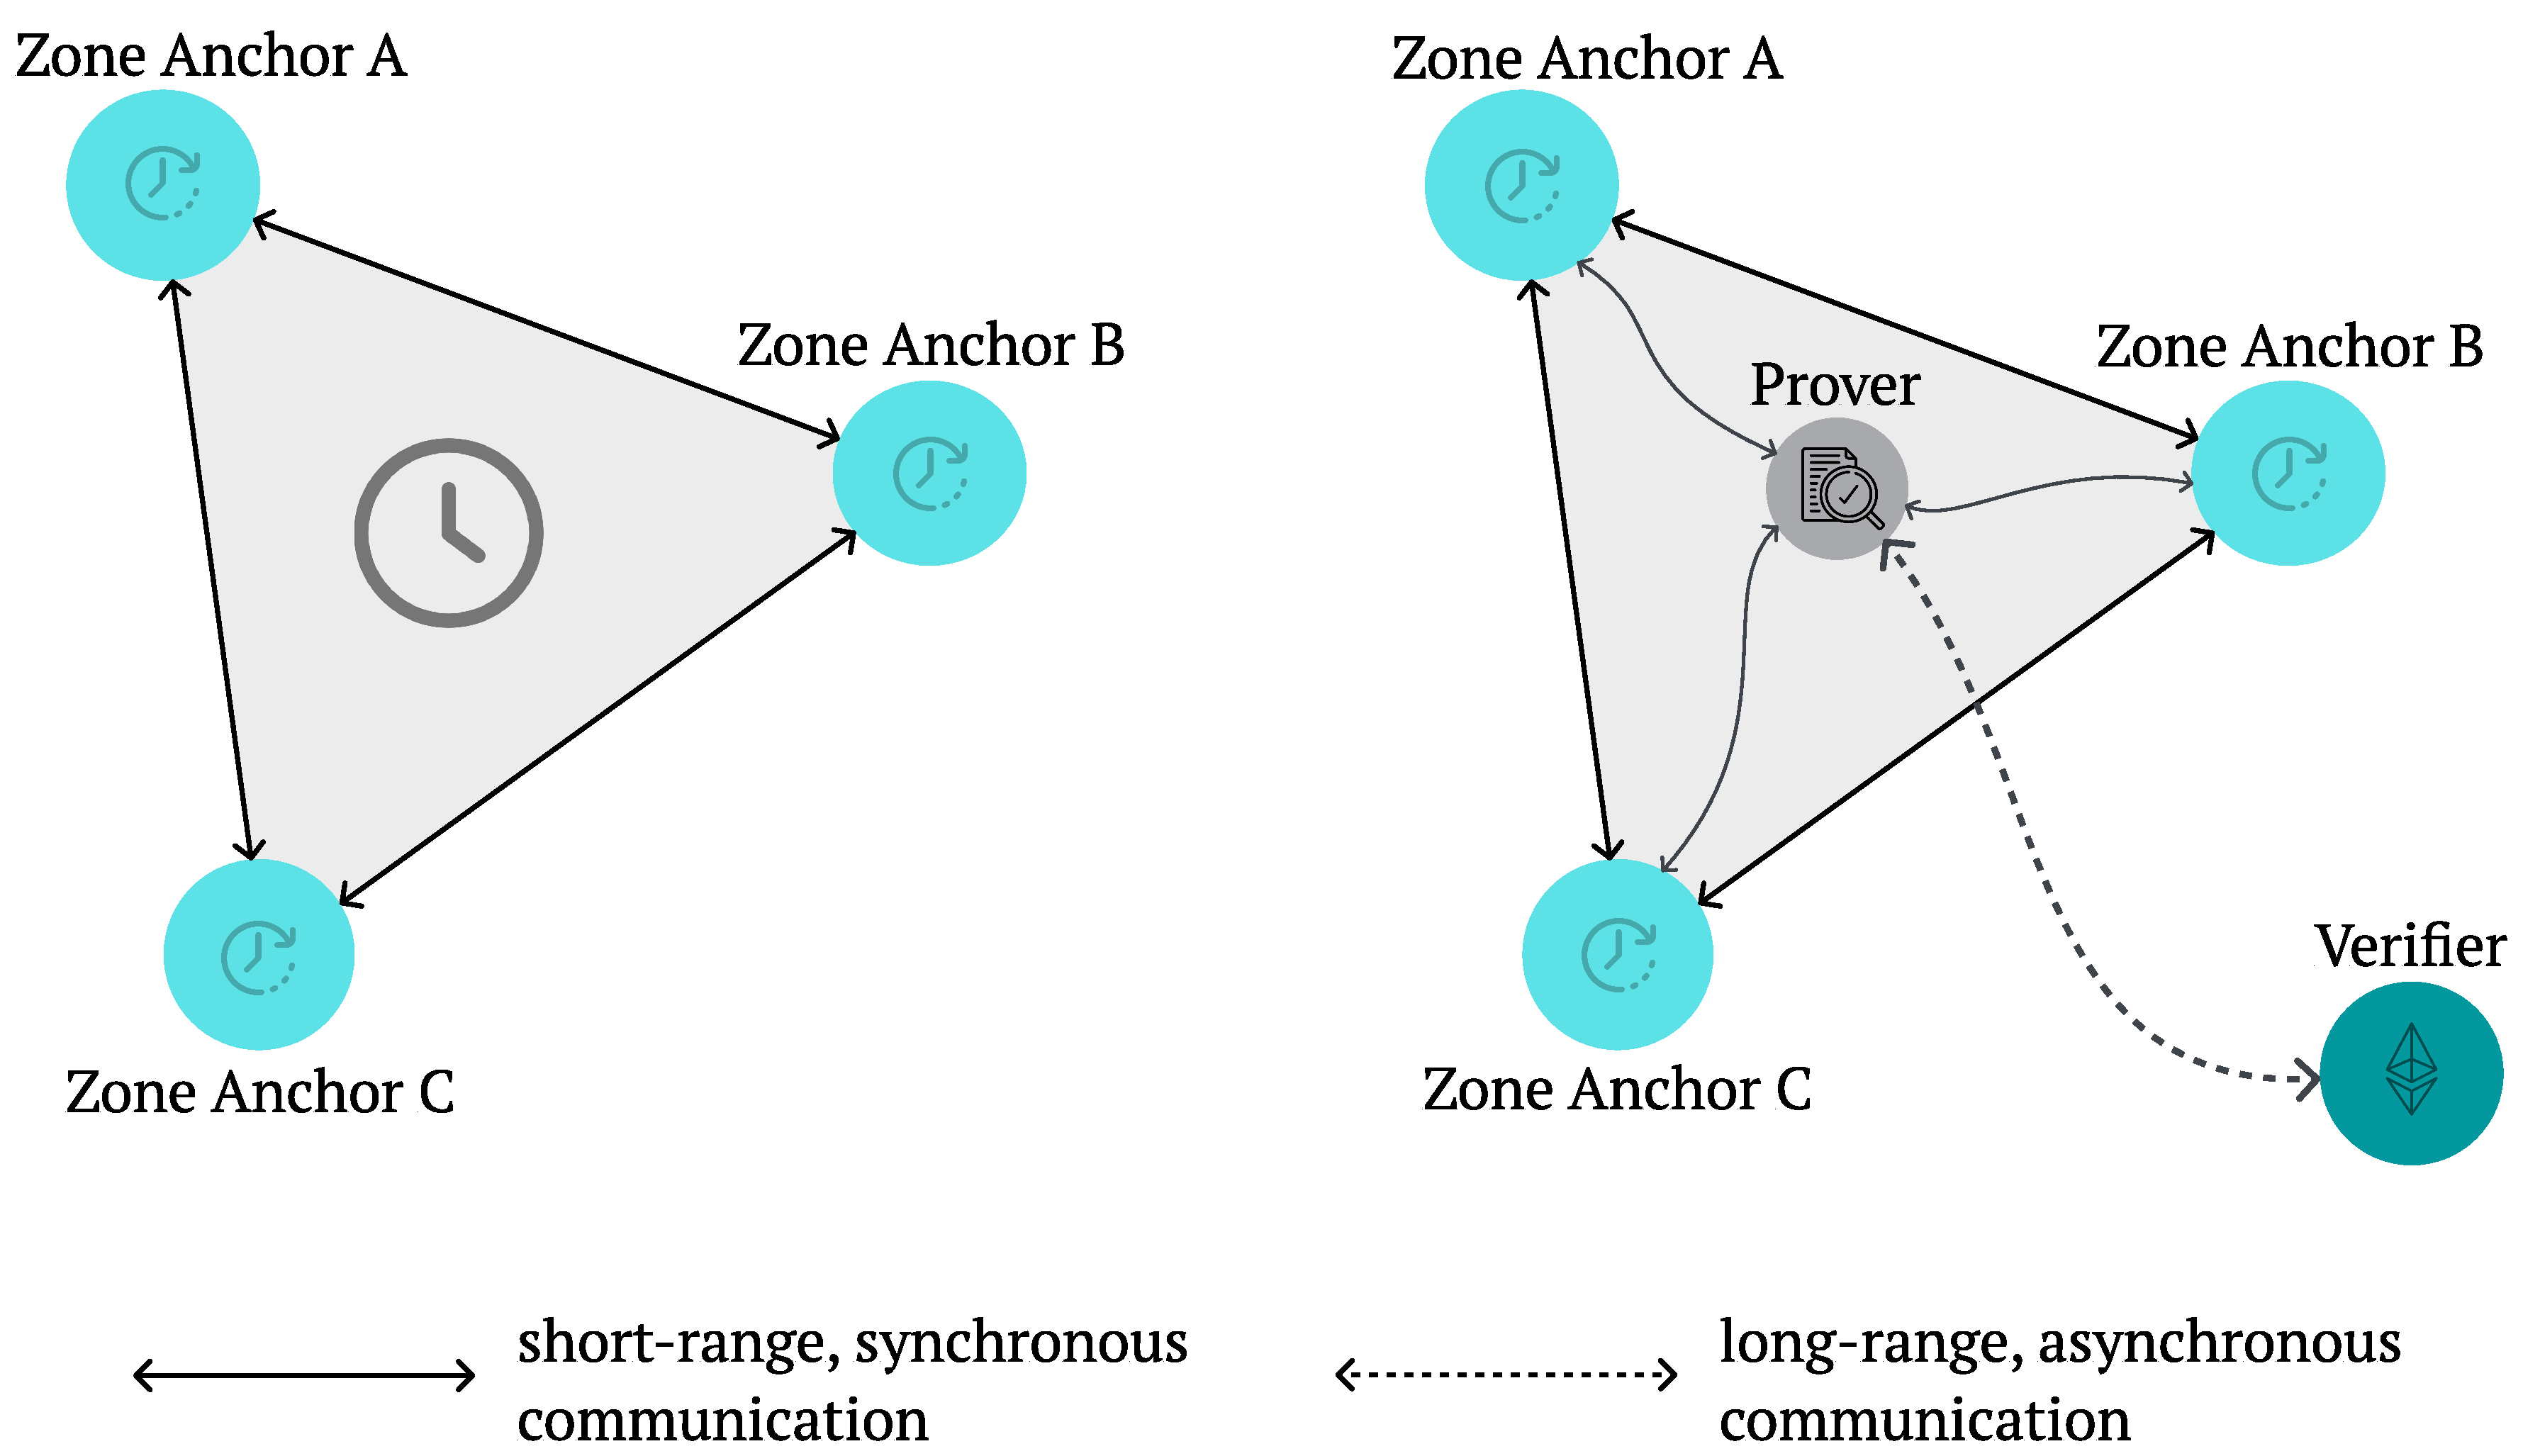
\includegraphics[width=0.9\textwidth]{trustless-pol.pdf}
    \caption{The FOAM protocol for dynamic and decentralized \pol{} \cite{foam-white-paper}.}
    \label{fig:trustless-pol}
    \end{center}
\end{figure}

\newpage

This chapter illustrated the evolution of \pol{} protocols, starting from centralized and trusted solutions and advancing towards decentralized and infrastructure-independent approaches. The distribution of trust has driven the development of modern protocols, culminating in the need for decentralized time synchronization, to make trustless witnesses collectively agree on attesting to the nearby presence of a prover. The FOAM protocol is the ultimate inspiration for the work developed further in this thesis. The processes of zone establishment, spatio-temporal synchronization, and decentralized witnessing consensus will be explored as in FOAM, but taking advantage of WiFi-based mesh networking, for the short-range exchange of information, and by employing a permissionless consensus mechanism, aligned with the concepts introduced in Sections~\ref{sec:background-wireless-mesh-networks}~and~\ref{sec:background-permissionless-consensus}.

% \subsection{Alternative Strategies} \label{sec:related-work-alternative-strategies}

% Inspired by the solution proposed by Zhu and Cao \cite{zhu2011applaus}, Amoretti et al. \cite{amoretti2018blockchain} dive into the definition of a novel decentralized and infrastructure-independent approach that allies together short-ranged communication technology and Blockchain-based storage and information verification. The authors propose the establishment of a distributed overlay network of linked nodes that, at the same time, wirelessly provide or request location proofs from nearby nodes, and verify or store propagated proofs, via any typical lower-level blockchain protocolar agreement, achieving, thus, permissionless consensus. Their solution is claimed to be one of the very first at protecting against the main location-based-systems' attacks, with the help of a fully decentralized and blockchain inspired peer-to-peer scheme, assuring both integrity and user privacy. Real-world performance evaluation and the possibility for integrating higher-level incentive mechanisms were set as future work prospects. Both Amoretti et al. \cite{amoretti2018blockchain} and Nasrulin et al. \cite{nasrulin2018robust} contemporaneous works illustrate practical constructs that take advantage of the tamper and censorship resistant nature of blockchain technology. The latter tries as well to formalize the main security and spatio-temporal requirements that such a decentralized \pol{} protocol shall present, as seen in Section~\ref{sec:background-proof-of-location}, ending up implementing a \poc{}, based on a permissioned blockchain framework, to specifically solve the challenges related to supply chain tracking.

Further efforts that build upon the above-mentioned solutions are the ones proposed by Wu et al. \cite{wu2020blockchain} and Nosouhi et al. \cite{nosouhi2020blockchain}. The first follows the path of Amoretti et al. \cite{amoretti2018blockchain} and tries to enable, on top of it, user-defined hierarchical privacy protection, with the help of Zero-Knowledge proofs. The proposed protocol finds a bridge between the typical \pol{} set of entities and the usual Zero-Knowledge proof participants. The suggested Zero-Knowledge \pol{} (zk-PoL) protocol aims at allowing the prover to convince the verifier that one was at a specific location, at a certain point in time, but with a granular privacy preserving disclosure of the location proof details. The obvious motivation of the mechanism is to solve spam, traceability, and privacy concerns of publicly storing raw location information, especially within decentralized and public ledgers. Therefore, the scheme is, to a great degree, centred in the privacy assurances and not in the infrastructural aspects of the potential decentralization that it is built upon. Nevertheless, it sets a promising starting point for the introduction of privacy preserving technology in the realms of trustless \pol{} protocols. Optimizations and faster proof mechanisms are kept in the outlook and waiting to be explored. Nosouhi et al. \cite{nosouhi2020blockchain} stress out a different proximity checking mechanism, to protect against the still unsolved prover and witnesses collusions, while committing, as well, to privacy preserving location proof generation and storage, using public and decentralized blockchain technology. Their work has also an original integration of an incentive mechanism that rewards collaborative participants, in order to more strongly prevent the main known attacks. This sets an unprecedented track for the incorporation of these \pol{} protocols into the digital and decentralized economy that already runs, via Smart Contracts, on blockchain networks like Ethereum \cite{nosouhi2020blockchain, buterin2014next}. 

Taking the above into account, Pournaras \cite{pournaras2020proof} proposes the complementing concept of Proof-of-Witness-Presence as a key element in an augmented democracy approach to smart city development. This concept involves validating the accuracy of data collected through participatory crowd-sensing, by requiring physical presence at locations of interest. The author argues that this approach can foster greater citizen engagement and participation in public spaces, and can be incentivized through blockchain consensus and a crypto-economic design. The work acknowledges the limitations of current localization methods, such as GPS, and suggests the need for more advanced and secure location certificates, based on complex social proofs. The Proof-of-Witness-Presence model envisioned by Pournaras may rely on token curated registries and a fully trustless \pol{} protocol that, for instance, FOAM\footnote{\url{https://foam.space/}} tries to deliver. The next paragraph will examine the main concepts of the FOAM protocol.

% The theorization of the singularity of a four-dimensional manifold, combining the three dimensions of space with the asymmetric arrow of time, has fundamentally shaped humankind's understanding of physical reality. The establishment of an absolute quorum over space and time is the ultimate goal that has driven forward the development of modern globalization, by the way we coordinate and synchronize our existence. Since the institution of the canonical time, sailing through the acknowledgment of the Longitude problem, to finally setting up intercontinental time synchronizers, the absence, or maintenance impossibilities of a truly global and absolute clock is still a major drawback in the production of correct, tamper-resistant, and spatio-temporally sound location information. 

Asserting the fundamentality of time synchronization, FOAM leverages Einstein's relativity hypothesis to create a new means for measuring space and time, for cartography and map making \cite{king_2020}. Their protocol, combined with their attempt at standardizing location data, is a totally new conceptual way of achieving decentralized, privacy preserving, highly accurate, censorship resistant, verifiable, and secure \pol{}. \emph{Zone Anchors} and \emph{Zone Authorities} form a dynamic and decentralized network of radio beacons and gateways that reach consensus over the precise time of their clocks, establishing zone-relative clock synchronization. This allows for the formation of time conscious zones of witnesses that can simultaneously determine spacial arrangements and provide presence claims. Figure~\ref{fig:trustless-pol} depicts the expectation that Zone Anchors or Zone Authorities dynamically synchronize their internal clocks, establishing a smart contract's enforced physical coverage zone that offers trustless, but spatio-temporally sound location services. Zones may provide precise, verifiable, and secure \pol{} claims, with the precision determined by possible triangulation mechanisms. Combined with token curated registries and crypto-economic incentives, for the maintenance and growth of the decentralized infrastructure, FOAM ultimately aims at creating a global consensus-driven map of the world. Their hopes are on Low Power Wide Area Network (LPWAN) radio technology, for the communication means, and on Ethereum-based Smart Contracts, for decentralized verification, consumption, and incentivization of the protocol operations over the location data \cite{foam-white-paper}.

\begin{figure}[ht]
    \begin{center}
    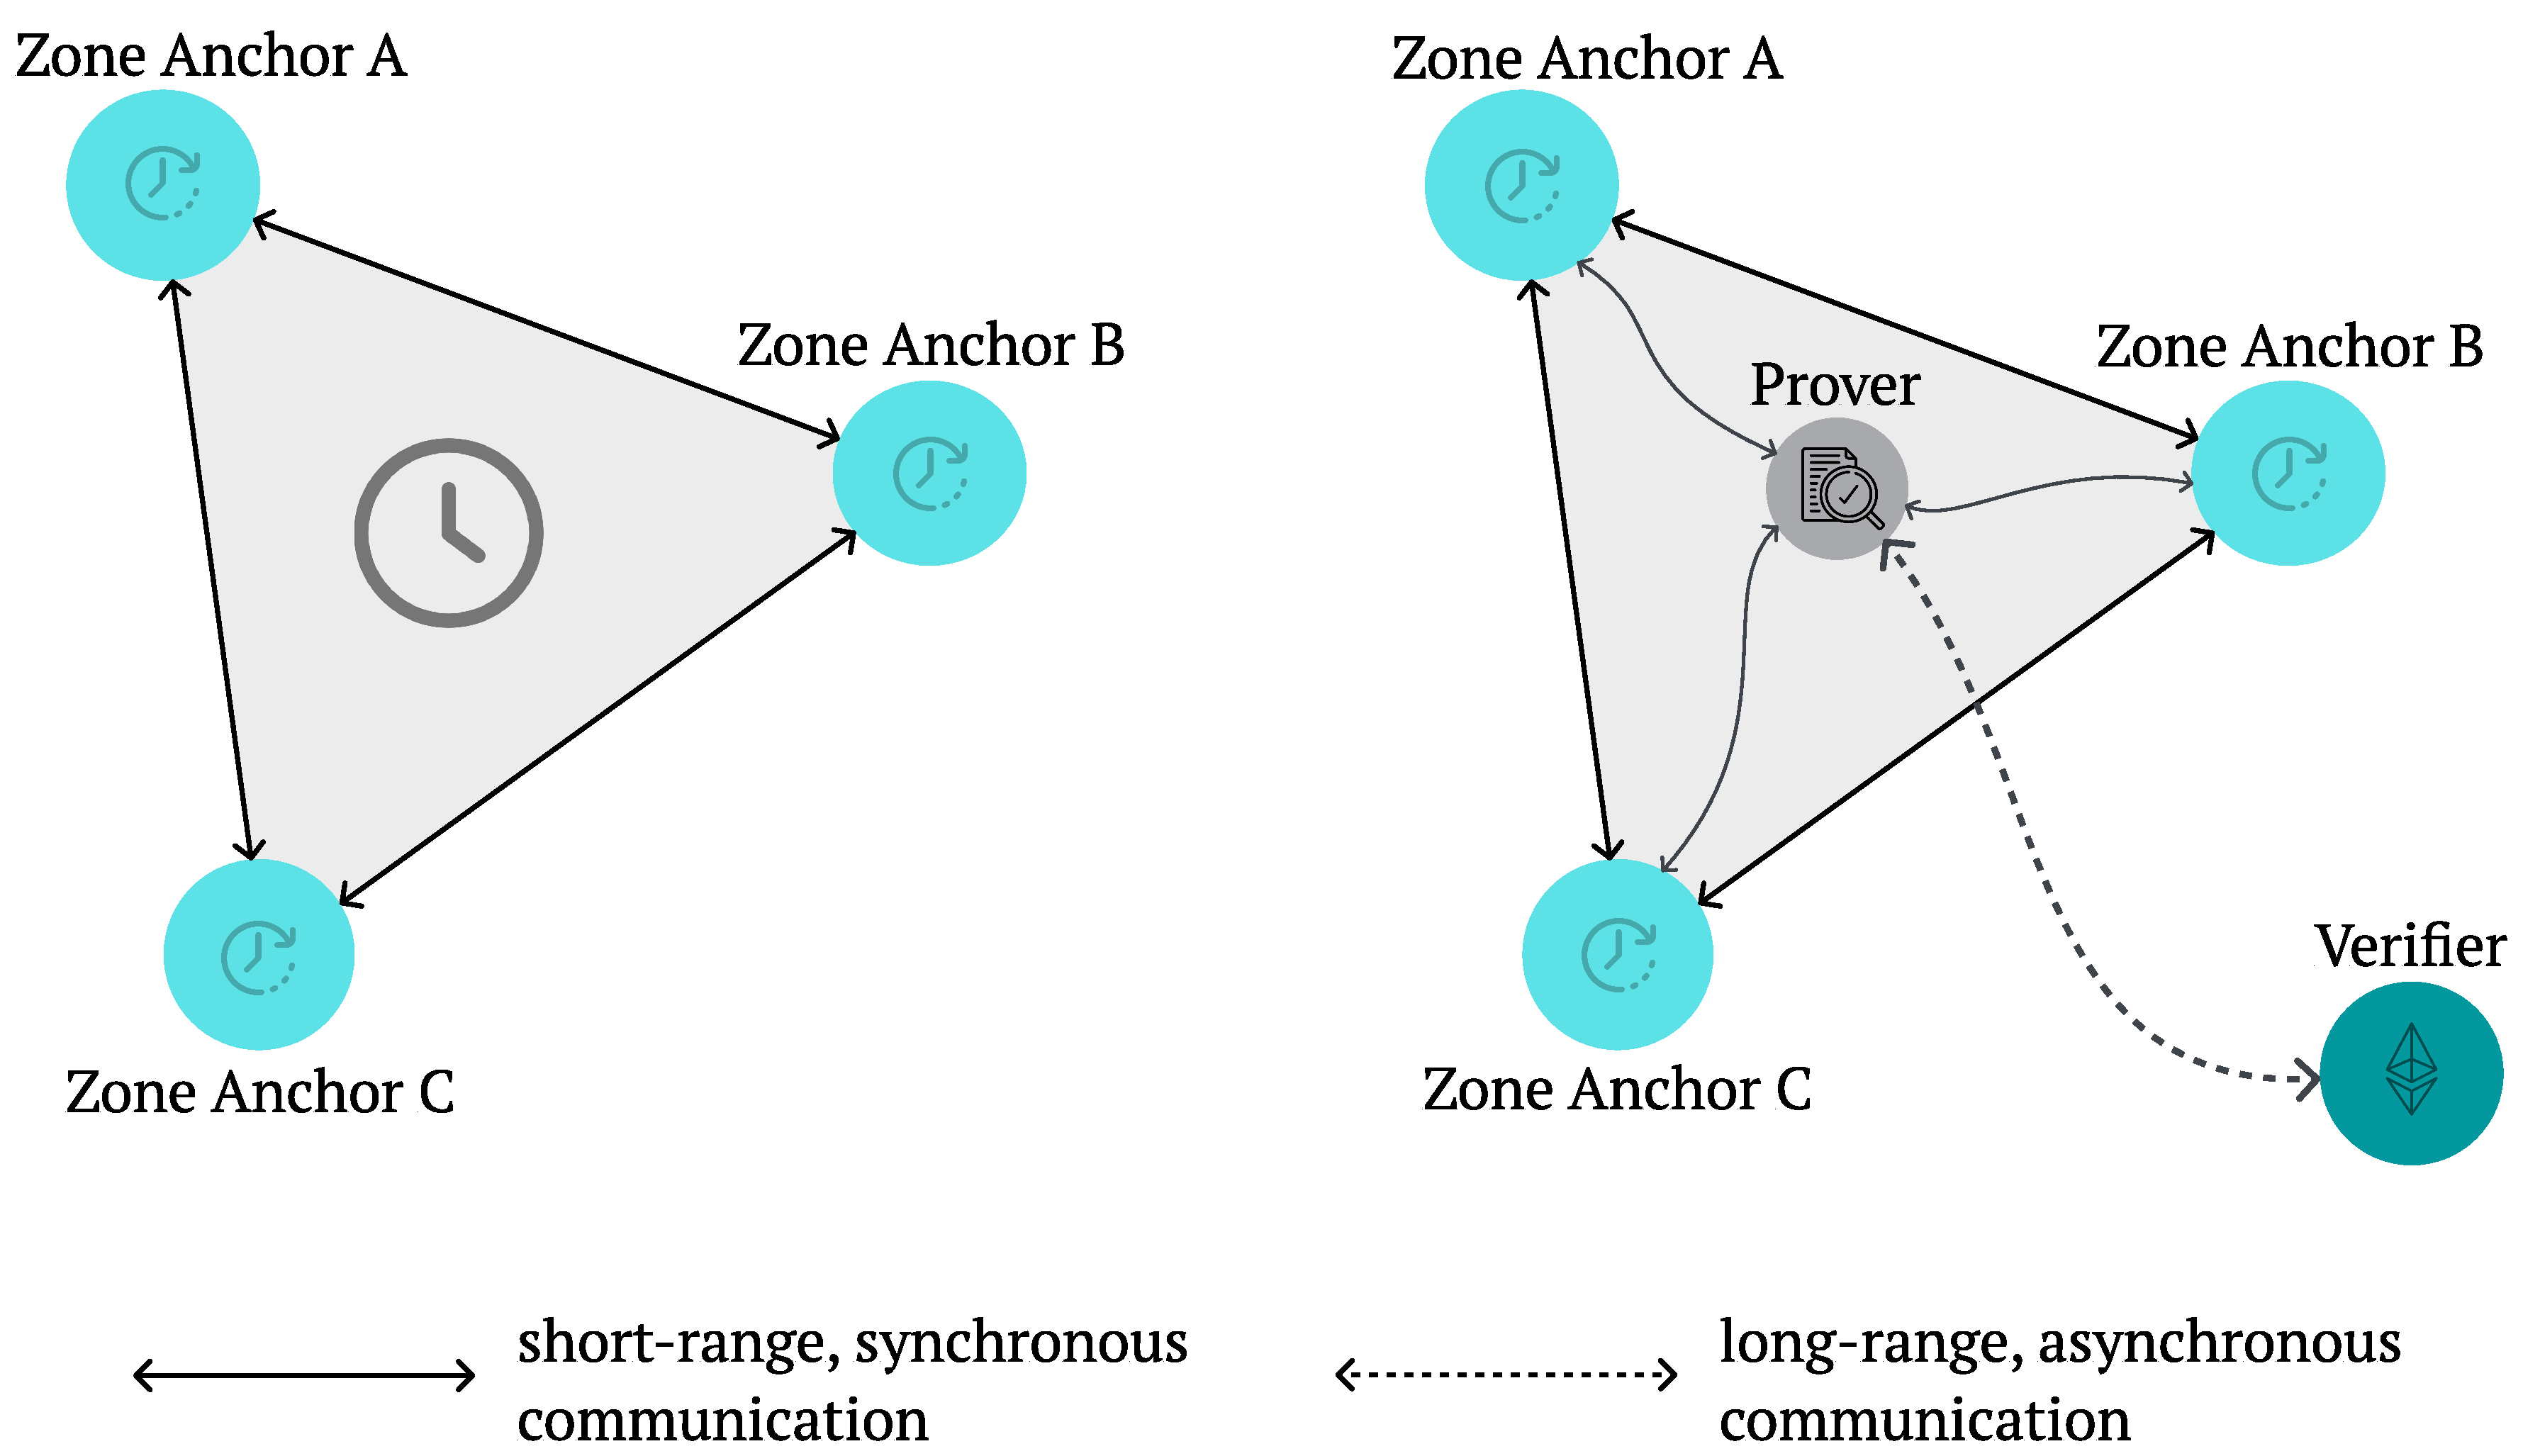
\includegraphics[width=0.9\textwidth]{trustless-pol.pdf}
    \caption{The FOAM protocol for dynamic and decentralized \pol{} \cite{foam-white-paper}.}
    \label{fig:trustless-pol}
    \end{center}
\end{figure}

\newpage

This chapter illustrated the evolution of \pol{} protocols, starting from centralized and trusted solutions and advancing towards decentralized and infrastructure-independent approaches. The distribution of trust has driven the development of modern protocols, culminating in the need for decentralized time synchronization, to make trustless witnesses collectively agree on attesting to the nearby presence of a prover. The FOAM protocol is the ultimate inspiration for the work developed further in this thesis. The processes of zone establishment, spatio-temporal synchronization, and decentralized witnessing consensus will be explored as in FOAM, but taking advantage of WiFi-based mesh networking, for the short-range exchange of information, and by employing a permissionless consensus mechanism, aligned with the concepts introduced in Sections~\ref{sec:background-wireless-mesh-networks}~and~\ref{sec:background-permissionless-consensus}.

\newpage
\section{Protocol Fundamentals} \label{sec:protocol-fundamentals}

This chapter outlines the key requirements and long-term goals of the proposed \pol{} protocol. It also provides an overview of the thesis' objectives, while aiming at contextualizing the subsequent technical work.

\subsection{Overview} \label{sec:protocol-fundamentals-overview}

The general approach to the design of \pol{} protocols has been mainly focused on the proof generation process, as seen in the multiple examples dissected in Chapter~\ref{sec:related-work}. Advancements made towards more distributed and decentralized solutions have highlighted the need for a comprehensive and detailed description of the protocol's entire range of requirements. To achieve an operable system that meets the demands of real-world applications, a phased strategy with a keen awareness of the intrinsic details, at every stage of the solution, is essential for providing a complete and coherent picture of the protocol's design. Therefore, we will attempt at the design of a \pol{} protocol that starts with an infrastructural foundation, and ends with a complete system~\textemdash~aiming to achieve the goal of proving one's location.

\begin{figure}[ht]
    \begin{center}
    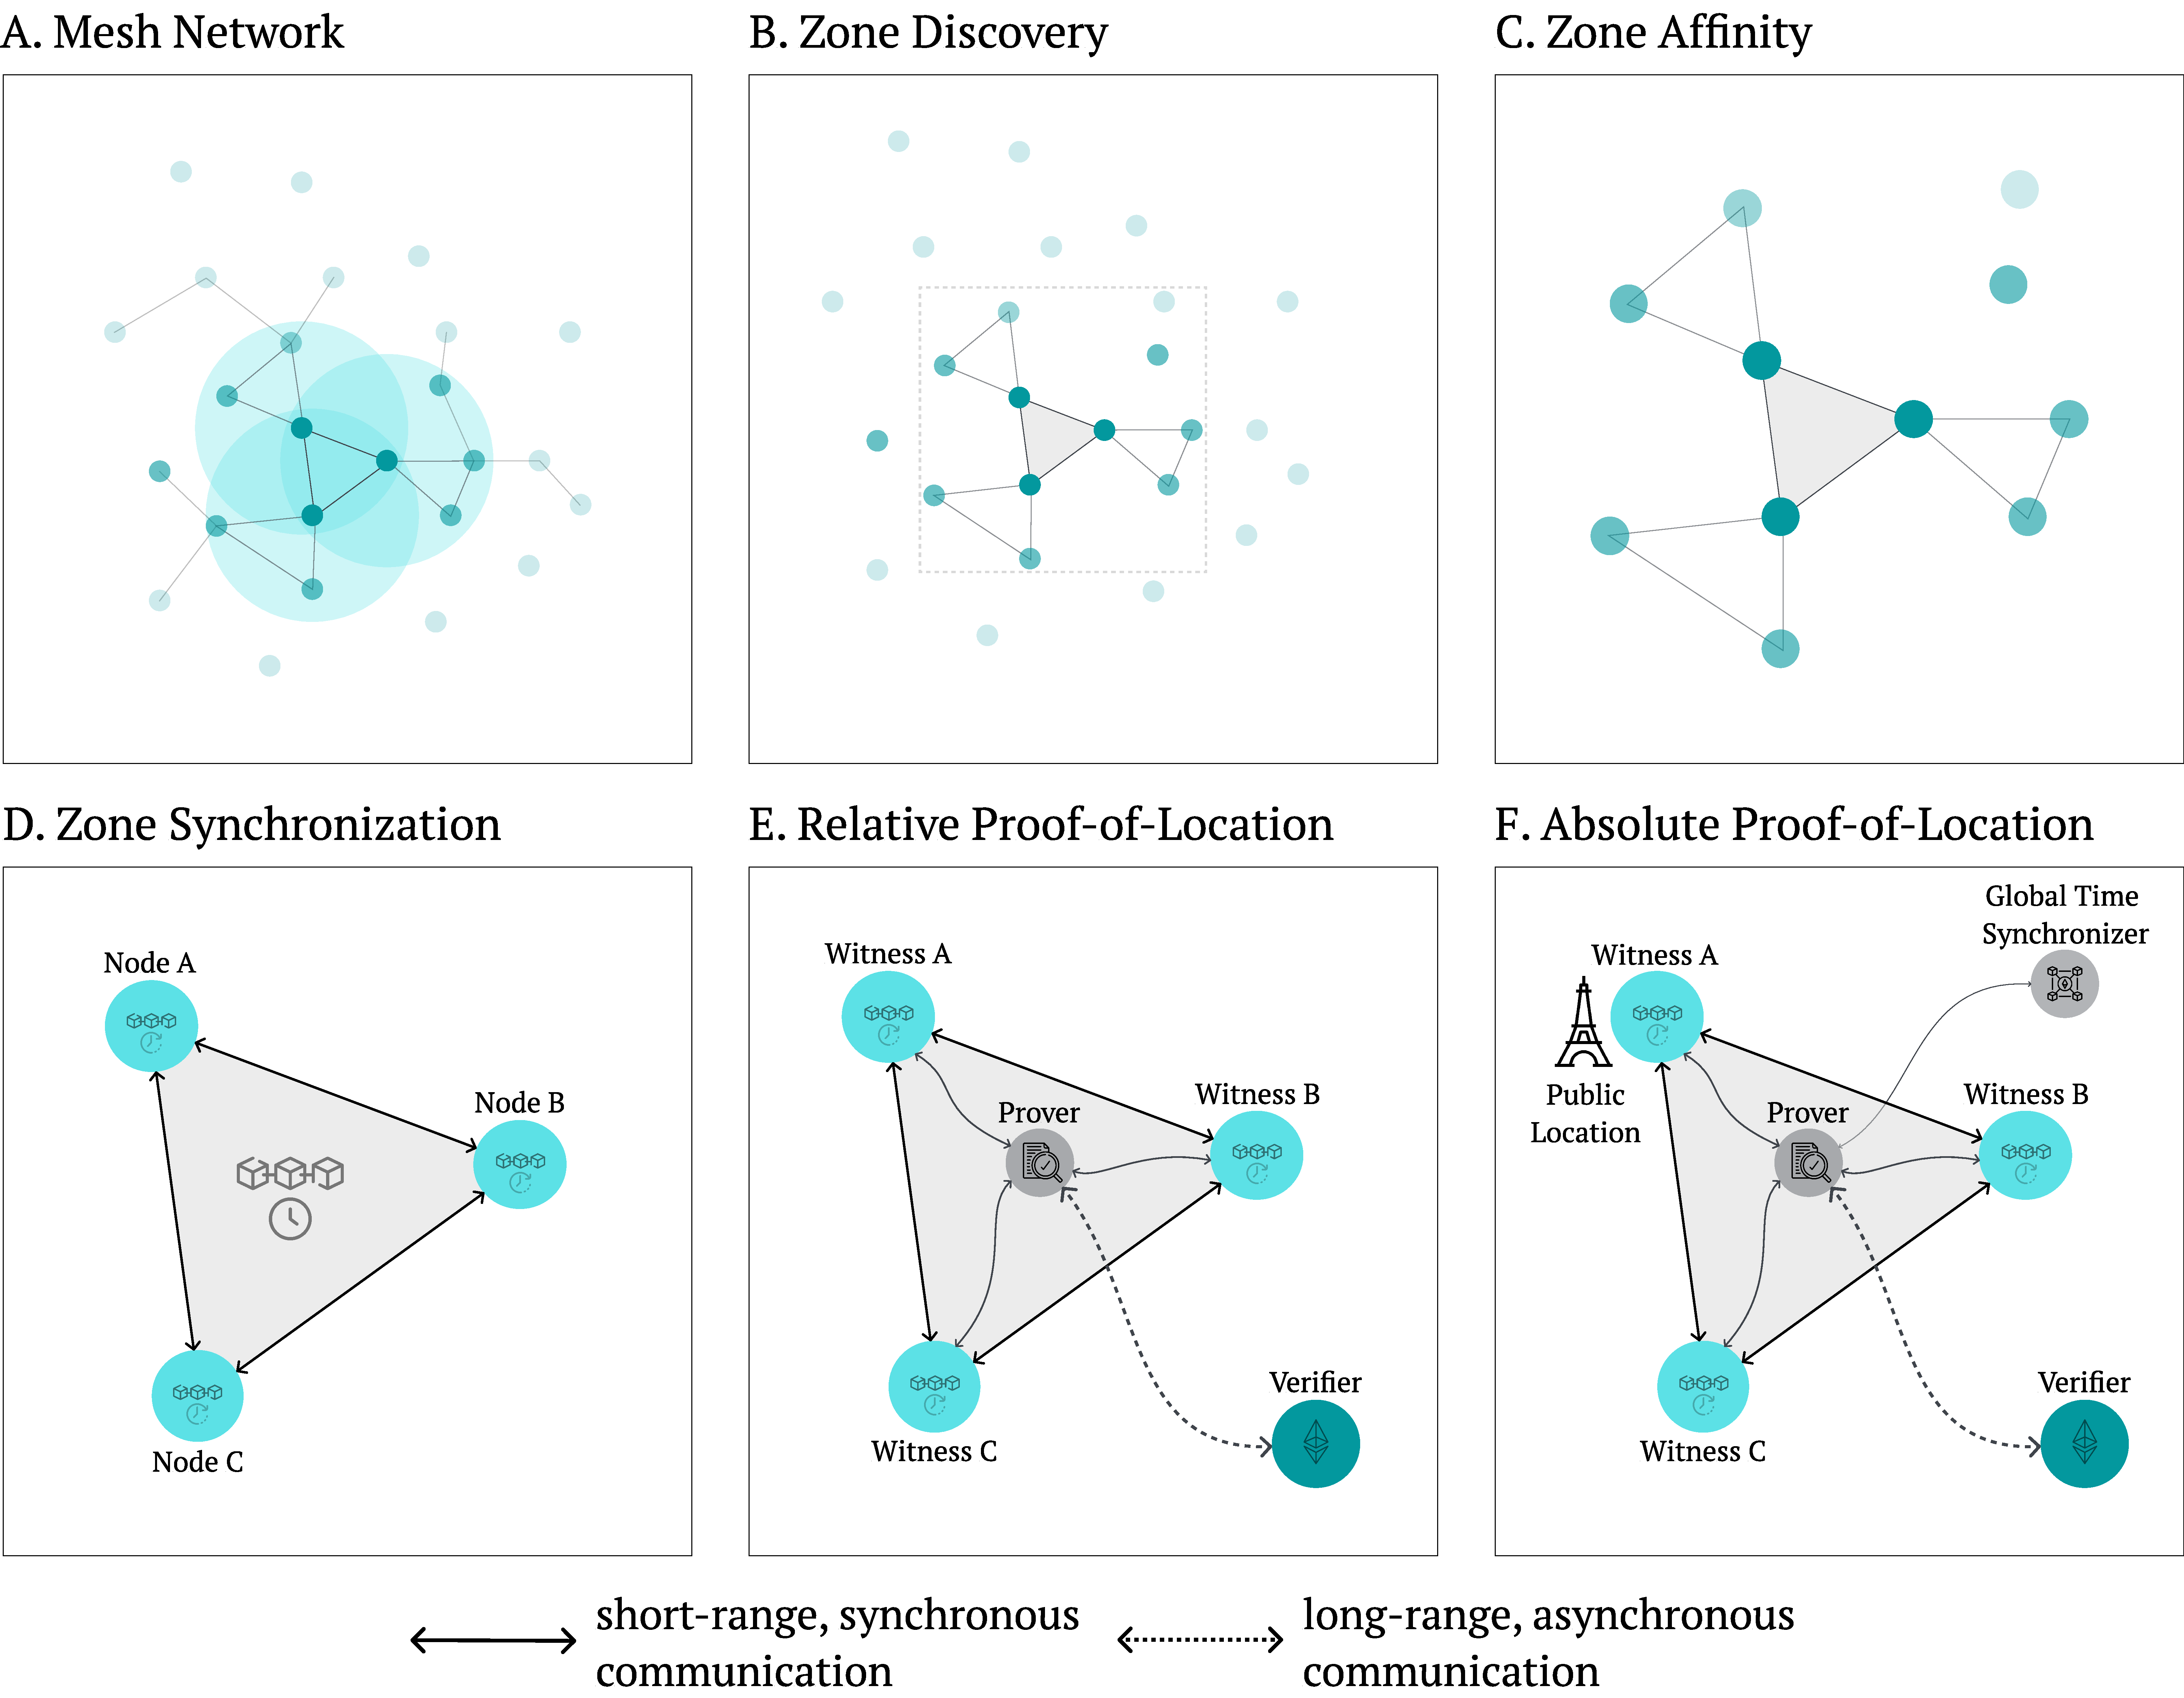
\includegraphics[width=0.9\textwidth]{overview-pol.pdf}
    \caption{A discretization attempt to capture the multiple steps of the protocol design, from a dynamic mesh topology, towards the ultimate goal of achieving Absolute \pol.}
    \label{fig:proof-of-location-overview}
    \end{center}
\end{figure}

The following sections will guide the reader through the multiple steps of the protocol's design. This journey, depicted in Figure~\ref{fig:proof-of-location-overview}, starts with the foundation layer of the system, powered by a dynamic and non-hierarchic Mesh Network topology. This topology should enable the network agents to communicate with each other in a peer-to-peer, short-ranged, and conveniently wireless fashion. The next step entails the nodes' neighbourhood establishment, eased by lower-layer routing protocols, leading to the eventual creation of fully connected zones of neighbours. Each node, however, may simultaneously belong to multiple zones, with the processes of zone affinity, zone switching, zone expanding, and, consequently, the overall configuration of the mesh topology being dictated by protocol requirements. Application-level incentives, in the lines of the ones envisioned in the FOAM protocol, may also take part in encouraging the formation of zones and growth of the network. The goal is to achieve a latticework of space and time, with zone-relative clock precision. Therefore, the next step is to establish, or derive, spatio-temporal zone synchronization. Space synchrony is accomplished with the assumptions regarding the short-ranged communication means. To achieve time synchrony, a clock synchronization mechanism is necessary. This mechanism not only ensures the synchronization of the witnesses' internal clocks, but can also enable zone-relative event serialization, via a strongly consistent consensus-based system. Moreover, by choosing and employing a Turing-complete consensus protocol, it becomes possible to execute more complex logic alongside these functionalities, for instance, with the deployment of smart contracts that potentiate the creation of decentralized and zone-relative location services. Nonetheless, the main aim is to achieve zone-relative time consciousness, to then enable spatio-temporal soundness and provide complete location proofs \cite{nasrulin2018robust}.

In the following sections, we will provide a more detailed analysis of these multiple steps. However, in the practical work, we will focus only on a subset of the entire problem. For the implementation of the \poc{} in Chapter~\ref{sec:proof-of-concept}, it is assumed that the processes of zone discovery and zone affinity management have already been accomplished, and the nodes have agreed to form a zone. The steps that follow the goal of achieving relative \pol{} are also left for future work.


\subsection{Dynamic and Non-Hierarchic Mesh Networks} \label{sec:protocol-fundamentals-mesh}

The envisioned fourth industrial revolution has set the track for modern advancements in achieving a global web of pervasive connectivity between all sorts of machines \cite{akyildiz2005wireless, cilfone2019wireless}. New means of radio and wireless communication have been pushing for the technological heterogeneity of protocols, architectures, devices, and consequent performance levels, in order to find their design suitability for different coverage or range scenarios, transmission or bandwidth rates \cite{sichitiu2005wireless}. Additionally, requirements for more complex, adaptable, and resilient topologies have captured broad interest, in both academic and industry domains. 

The development of new hardware, protocols, and applications started gaining momentum and branched their way forward to support the popularisation of Wireless Mesh Networks (WMNs). In mesh topologies (see Figure~\ref{fig:mesh-network-topology}), network nodes are directly and dynamically connected in a non-hierarchical way. This trait eventually allows for many-to-many communications between the devices, to efficiently route data from a generic source to a generic destination. The infrastructure nodes that make up the mesh are expected to dynamically self-organize and configure themselves, resulting in beneficial distributed effects on the overall fault tolerance, ease of deployment, and workload allocation \cite{cilfone2019wireless, sichitiu2005wireless}. WMNs follow these principles with the particularity of being made up of radio nodes that communicate via any sort of wireless means.

\begin{figure} [h!]
  \begin{center}
  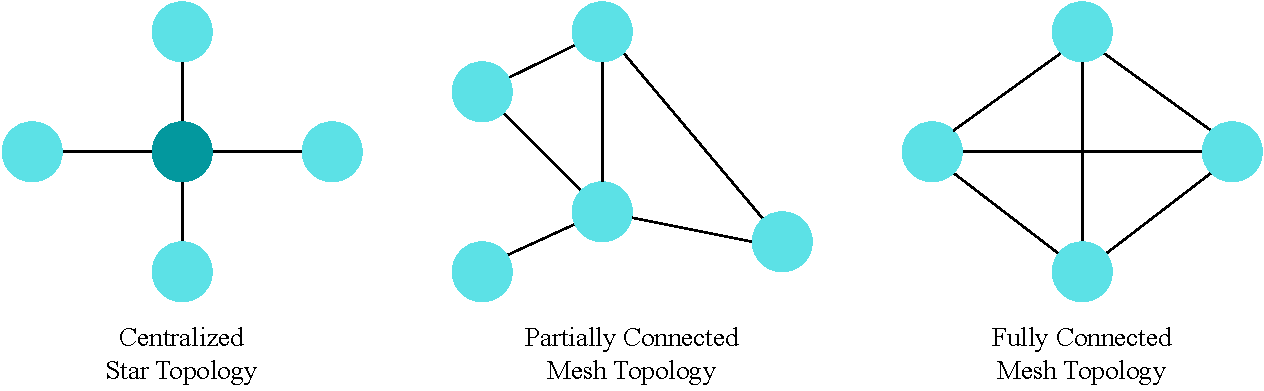
\includegraphics[width=0.8\textwidth]{network-topologies.pdf}
  \caption{Examples of different topologies of a computer network. Starting on the left, the star topology shows all the nodes connected to a central hub. To the right, examples of mesh topologies depict the direct and decentralized connections between the nodes.}
  \label{fig:mesh-network-topology}
  \end{center}
\end{figure}

Some of the most common technologies that have been, throughout the years, ported to WMNs are Bluetooth, LoRa and IEEE 802.11. The first two are prominent solutions for the extremities of the mesh networking spectrum, with Bluetooth under the short-range realm of Personal Area Networks (PANs), and LoRa  under the Low Power, Wide Area (LPWA) scenario. Downsides of these technologies are, respectively, the limiting coverage range for one-hop neighborhoods, or the low bandwidth rates \cite{cilfone2019wireless}. Hence, IEEE 802.11 became the most flexible and widely used technology, being the basis of the Wi-Fi standard, which, at the beginning of the last decade, saw an amendment that mainly targeted mesh networks~\textemdash~the IEEE 802.11s WLAN Mesh Standard \cite{hiertz2010ieee}. The novelty came with the introduction of routing mechanisms operating at the ISO/OSI Layer 2, allowing for compatible information delivery in the layers above. The dynamic establishment of a topology for IEEE 802.11s-based mesh networks relies on the phased transmission of beacon messages that allow for the discovery, synchronization, and maintenance of the links between the peers. IEEE 802.11s has a default routing protocol, the Hybrid Wireless Mesh Protocol (HWMP), which is based on a series of flooding procedures for both proactive and reactive path finding and selection \cite{bari2012performance}. However, this protocol is not strictly enforced by the standard and has been replaced by other more popular solutions. One notable example is the Better Approach To Mobile Ad-hoc Networks (B.A.T.M.A.N.) routing protocol.

This thesis will explore the concept of mesh networks and their potential for serving as the infrastructural topology that enables the relatively short-ranged exchange of messages between the participants of a \pol{} protocol. The following sections will present the B.A.T.M.A.N. routing protocol, OpenWrt, and other relevant tools that will be later used to implement the \poc{}.

\subsubsection{B.A.T.M.A.N. Routing Protocol}

The Better Approach To Mobile Ad-hoc Networks (B.A.T.M.A.N.)\footnote{\url{http://www.open-mesh.org/}} is a proactive routing protocol for WMNs, operating at the data link layer instead of the network layer, asserting the reliability of radio links using routing metrics and a distance-vector approach \cite{seither2011routing}. Its newer version, \emph{batman-adv}, has gained traction and popularity and eventually made itself available in the Linux kernel.

Route discovery is preemptively replaced with neighbour discovery, and each infrastructural node is instructed to calculate its potential best next-hop, significantly reducing the overhead of requiring each peer to be aware of the whole network topology. Its version V introduced a throughput metric to evaluate the links' quality and routing choices, replacing version IV packet-loss metric, deemed unsuitable for larger network sizes \cite{seither2011routing}.

\begin{figure} [ht]
  \begin{center}
  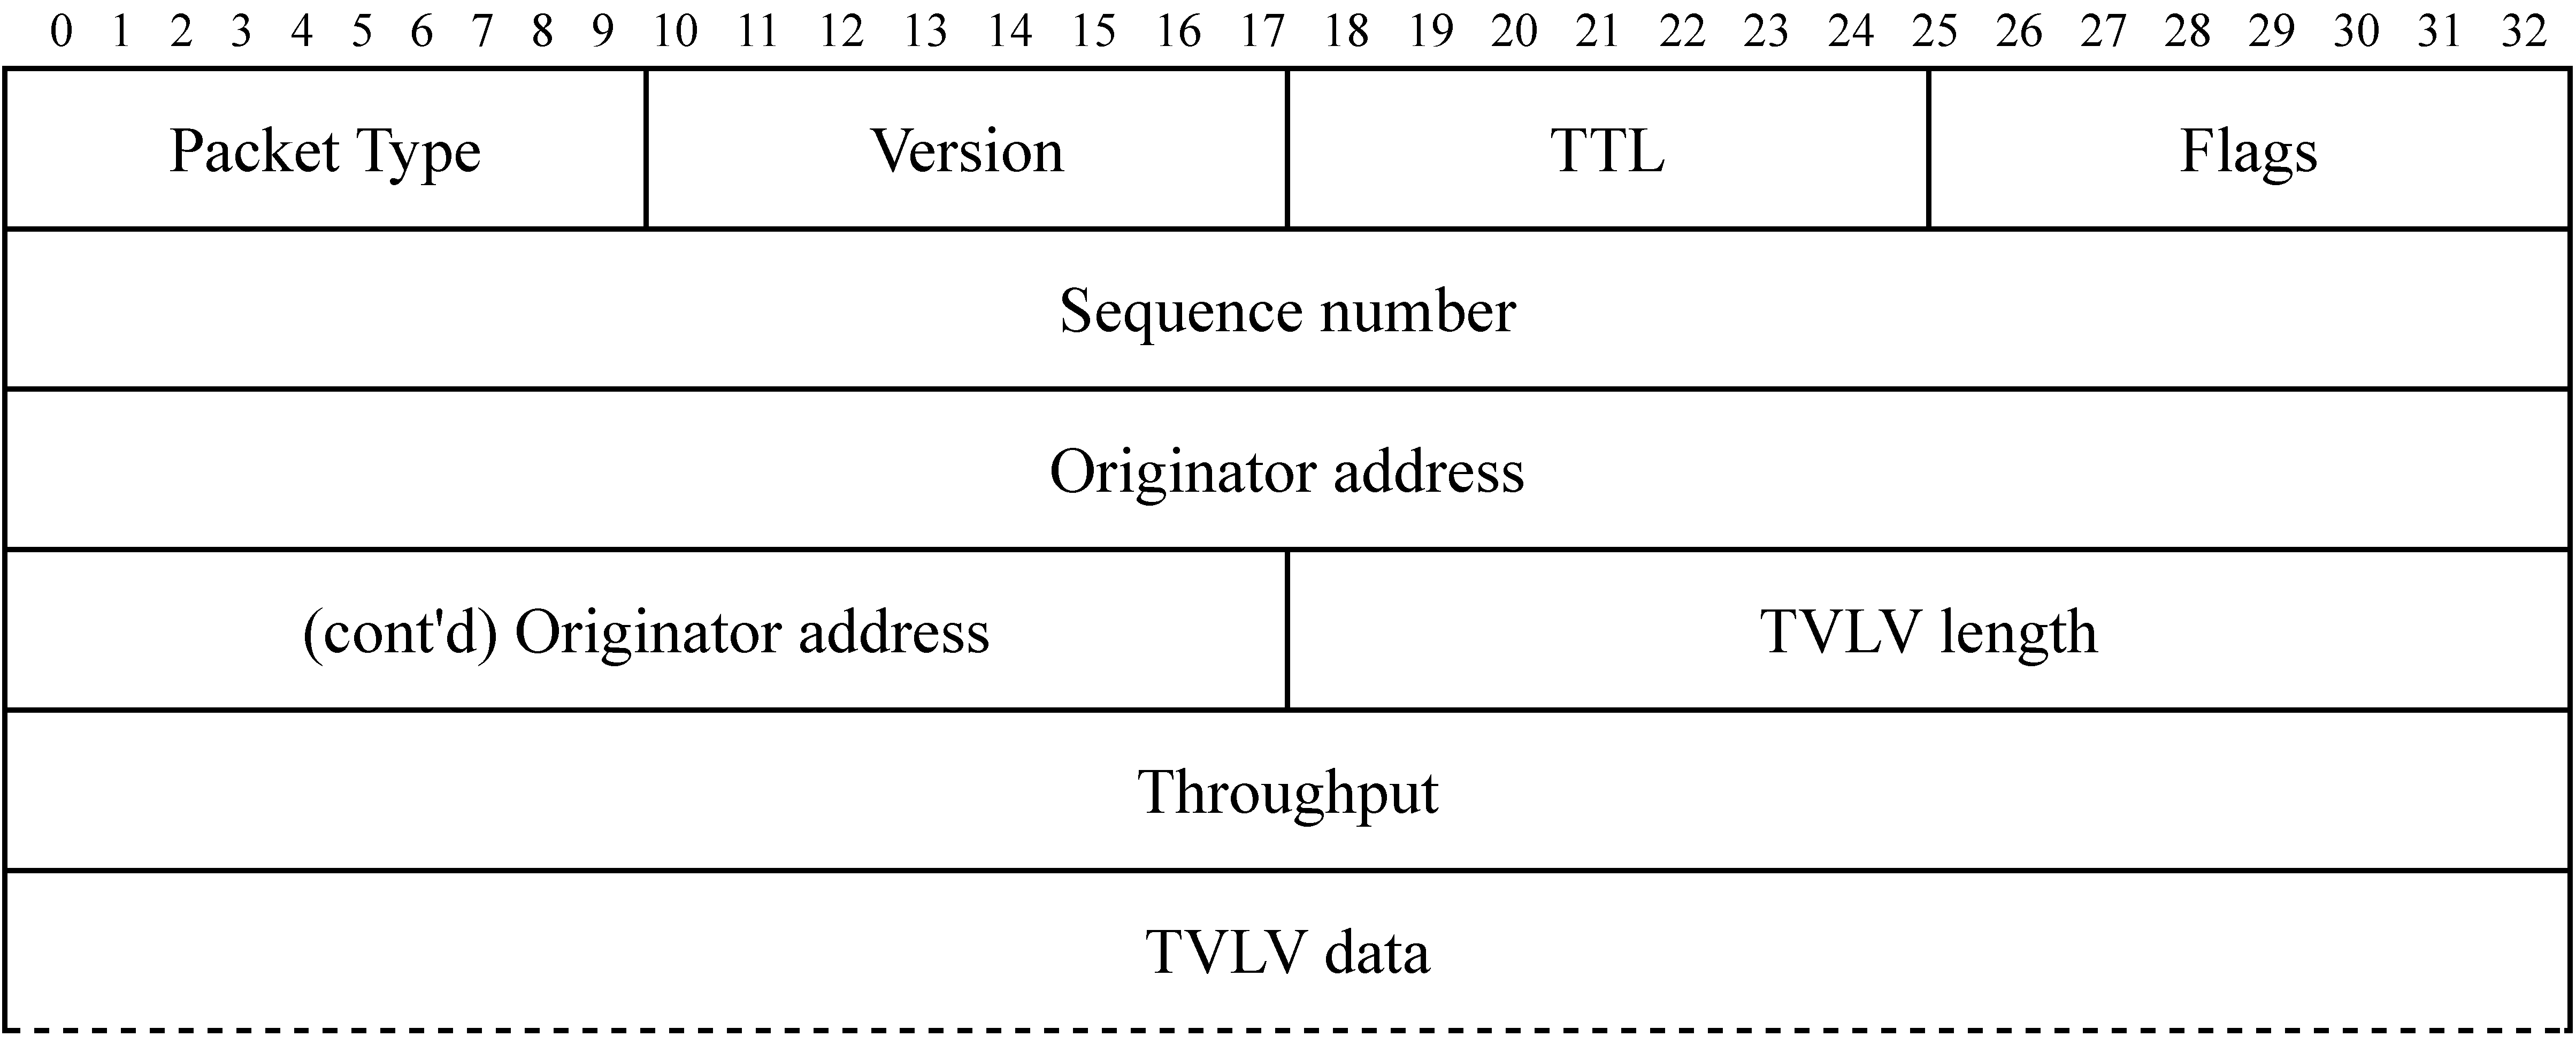
\includegraphics[width=0.9\textwidth]{batman-adv-ogmv2.pdf}
  \caption{OriGinator Message version 2 (OGMv2) packet format \cite{cilfone2019wireless,open-mesh-ogmv2}. These messages are broadcasted with a collision avoidance delay mechanism defaulting to 1 second. The packets contain, among other fields, the originator's MAC address and throughput metric values, measured in units of 100 kbit/s.}
  \label{fig:batman-adv-ogmv2}
  \end{center}
\end{figure}

The discovery of neighbouring nodes is accomplished with the capture of broadcasted OriGinator Messages (OGMv2, see Figure~\ref{fig:batman-adv-ogmv2}), that feature a collision avoidance delay mechanism, the detection of new or duplicate messages, and other fields for throughput measurement and gateway discovery. The Echo Location Protocol (ELP) handles the received messages and ranks the discovered neighbours. The OGM flooding protocol, on the other hand, enables mesh routing procedures that, simultaneously but independently, allow for estimating the quality of the individual links \cite{cilfone2019wireless}. Additionally, the protocol facilitates OGM aggregations as an effort to reduce the overhead of sending many short-sized frames. Nevertheless, there is still a quest for optimizations that would allow for more efficient use of multiple interfaces. An implementation of a subset of the Internet Control Message Protocol (ICMP) is also made available, allowing, for instance, the use of the \emph{ping} command to test the connectivity between nodes \cite{seither2011routing}.

Building on the previous, the B.A.T.M.A.N. routing protocol has been, through multiple initiatives, successfully blended into the OpenWrt project, which will also be employed in the \poc{}. The following section will present OpenWrt and other relatable tools.

\subsubsection{OpenWrt, QEMU, and Raspberry Pis}

The OpenWrt project\footnote{\url{https://openwrt.org/}} is a Linux distribution for embedded devices, which, in the context of this thesis, will serve as the host operating system for running the \poc{} solution. The project is based on the Linux kernel, encapsulating several of its libraries and packages, and is designed to be used on resource-constrained devices. OpenWrt features not only a writable root filesystem and automated build tools with integrated cross-compiler toolchain, but also a package management system that allows for the installation of additional software. The project also provides extensive configuration options for networking capabilities, which includes enabling mesh networking support through the B.A.T.M.A.N. routing protocol. 

To facilitate the development and testing of the \poc{}, the QEMU\footnote{\url{https://www.qemu.org/}} emulator will be used. QEMU is a generic and open-source machine virtualizer that, through its versatile set of features, allows for the full-system emulation of a wide range of hardware and software. The emulator will run the OpenWrt generated images and spawn multiple virtual machines. These machines will simulate the various protocol participants by establishing, with the help of the network emulation tools, a fully connected mesh network. The intention is to ease and accelerate the development process by allowing for testing the \poc{} in a controlled environment, without the management, maintenance, and deployment hustle of physical devices. Later, the solution is planned to be deployed on a set of Raspberry Pis\footnote{\url{https://www.raspberrypi.org/}}, the most widely used single-board computers for developing IoT solutions. The implementation journey will be documented in Chapter~\ref{sec:proof-of-concept}.


\subsection{Turing-Complete Clock Synchronization} \label{sec:protocol-fundamentals-clock}

Section~\ref{sec:related-work-fully-trustless} has already outlined the invariable need for clock synchronization, when it comes to reach progressively more accurate, correct, sound, and tamper-proof means of location attestation. What has not been discussed yet is the bridge between the clock synchronization problem and the consensus problem, in the specific context of distributed systems. 

This section will briefly discuss how these two fundamental problems are, in fact, intertwined. In simple terms, synchronizing clocks is nothing more profound than reaching agreement about the current time of the internal clocks of a distributed setting of machines. The indiscriminate case of clock synchronization can be stretched to a continued act of counting time at the same pace, as the indiscriminate case of reaching agreement about the current time of the internal clocks can be extended to a continued act of reaching agreement about the current state of the system. The latter is the consensus problem, and the former is a special case of it, the case of time synchronization. As argued in Section~\ref{sec:background-permissionless-consensus}, craving to achieve time synchronization, in not just a distributed setting, but in a fully trustless environment, can be transposed to the problem of achieving permissionless consensus, fulfilling the need for ordering and synchronizing events, at the same pace, in an environment where individual participants are not necessarily trusted. The first example depicted in Figure~\ref{fig:proof-of-location-example-scenarios} makes it clear that the eyewitnesses can only attest to the reporter's presence at the accident site if they had been there at the same time and witnessed the same event. However, these entities are not necessarily known to each other and to anyone else around, nor are they necessarily trusted. This implies not trusting that the clocks of the witnesses are correctly adjusted, as well. Therefore, the witnesses need to reach agreement about the current time, in order to be able to collectively and correctly attest to the reporter's presence at the accident site, in a given moment, otherwise they would all have conflicting or different reports. Additional to that, they may also attest to the reporter's course of action, by the means of taking pictures or recording videos, which are also events that may be ordered and synchronized, achieving, thus, permissionless consensus.

In consequence and specifically regarding the \pol{} problem, the need for clock synchronization is not only a matter of achieving more accurate positioning measures, as typically done in GPS-related trilateration systems, but a fundamental matter of achieving complete and sound consensus between the witnesses that are set to attest to one's location. Fundamentally, as defined in Section~\ref{sec:background-proof-of-location}, a \pol{} is complete if the attestation is done at location $l$ and time $t$, by a set of witnesses $w \in W$. To cope, as well, with the proposed property of spatio-temporal soundness, these witnesses should invariably reach consensus. They should not just agree to exist at around the same location $l$, relative to the precision, reliability, and coverage of their physical communication means, but should also agree on the time $t$, relative to the precision of their internal clocks. The latter is exactly the clock synchronization problem, folded into the greater and abstract need for consensus. The FOAM protocol proposes the achievement of such a time agreement with the employment of a self-stabilizing hybrid fault-tolerant clock synchronization protocol \cite{foam-white-paper, malekpour2015self}. The authors justify the choice highlighting the formal verification methods employed in Malekpour's work. This distributed algorithm is expected to formally work to the extent of the presence of a one third minority of Byzantine nodes \cite{lamport2019byzantine}. This fact validates the theoretical need for a composition of at least four witnesses for the most basic configuration of a zone, in the FOAM protocol. 

\begin{figure}[b!]
    \begin{center}
    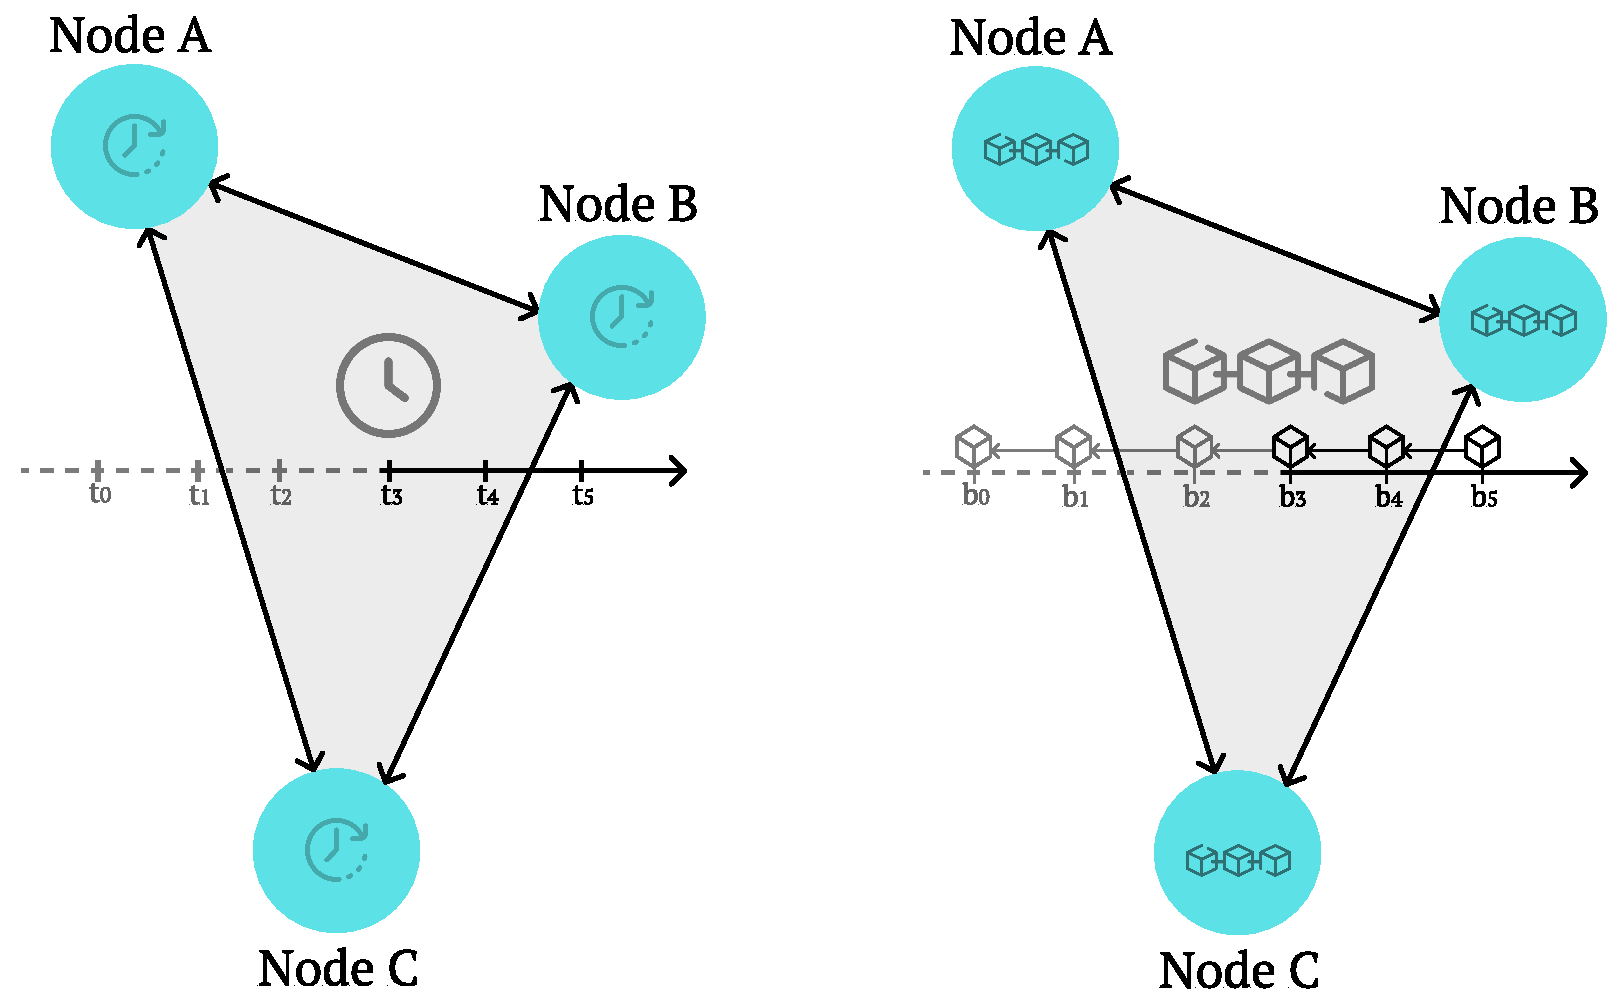
\includegraphics[width=0.8\textwidth]{overview-pol-time-sync.pdf}
    \caption{The goal of establishing zone-relative time consciousness, on the left, by the employment of a clock synchronization protocol, and on the right, by the employment of a consensus mechanism. Relative to the precision of both frequencies, the two mechanisms should achieve the same result, with the latter allowing for a strongly consistent serialization of transactions and total order of multidimensional information.}
    \vspace{-1cm}
    \label{fig:proof-of-location-overview-time-sync}
    \end{center}
\end{figure}

\begin{figure}[b!]
    \begin{center}
    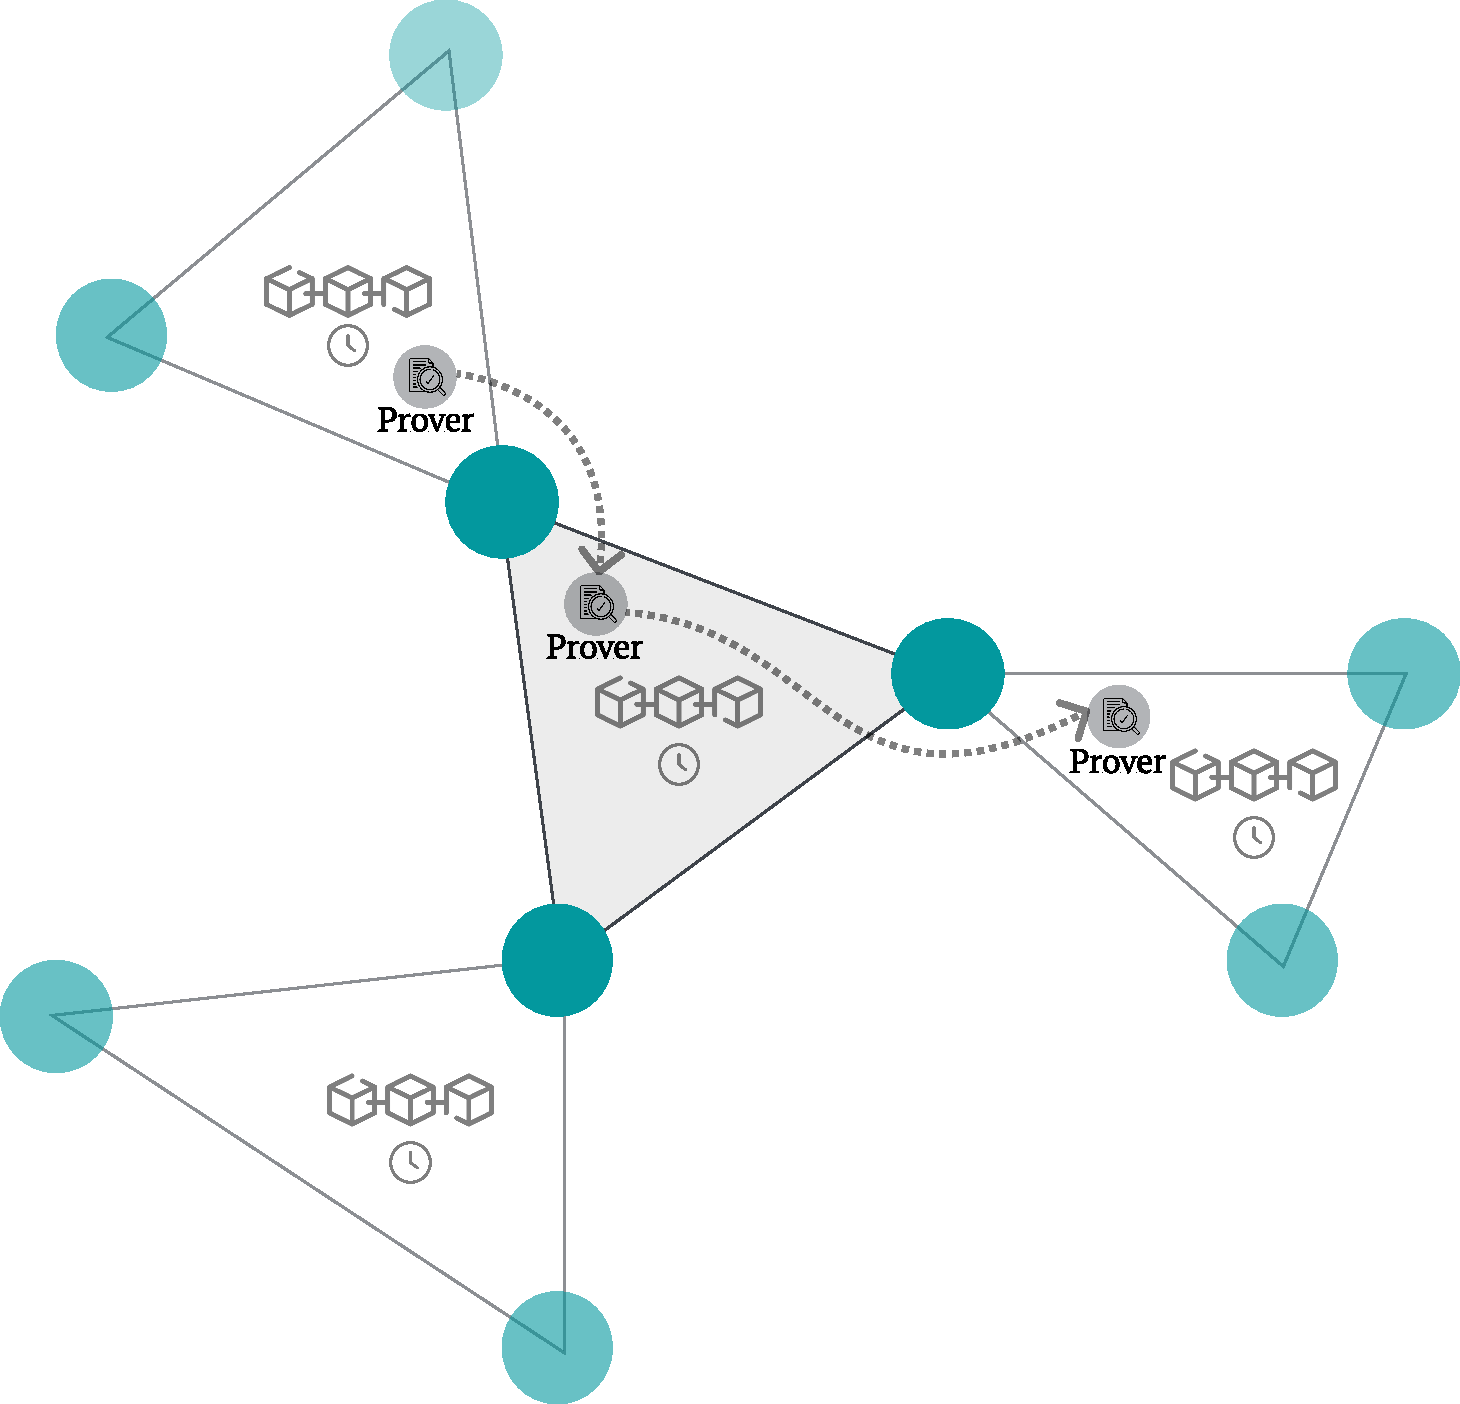
\includegraphics[width=0.6\textwidth]{overview-pol-latticework.pdf}
    \caption{The dense latticework of time-conscious witnessing zones, providing location services. Such a structure would allow for more accurate and verifiable location attestations, for example, regarding moving provers that constantly change their locations.}
    \vspace{-1cm}
    \label{fig:proof-of-location-overview-latticework}
    \end{center}
\end{figure}

This thesis proposes, instead, the empirical experimentation with a permissionless consensus mechanism, in the lines of the ones introduced in Section~\ref{sec:background-permissionless-consensus}. The goal, as illustrated in Figure~\ref{fig:proof-of-location-overview-time-sync}, is equivalent to establishing zone-relative time consciousness, but with the added benefit of providing strongly consistent serialization of transactions and total order of multidimensional events, instead of simply counting time in a unidimensional manner. The technicalities of modern systems that tackle the permissionless consensus problem allow, as well, for stronger guarantees in terms of security, tamper-proof and censorship resistance, as discussed in Section~\ref{sec:related-work-fully-trustless}. The fault-tolerance guarantees of a typical deterministic-finality Byzantine fault-tolerant algorithm are shifted back to a probabilistic finality fault-tolerance threshold, where the probability of a transaction being finalized is directly proportional to the number of nodes that have approved it \cite{survey-dist-consensus}. This is, arguably, a more desirable property for the considerations of a decentralized \pol{} protocol, where the finality of a location certificate is directly proportional to the number of witnesses that have seen the prover, and thus, the number of witnesses that have agreed on the time of the attestation, in the context of trustless environments. The methodical work of formally verifying, measuring, and comparing the two approaches, in the specific context of \pol{} protocols, is also left for future work. This thesis will plainly focus on the experimentation with a consensus mechanism that not only allows for the logical synchronization of clocks, via the regulation of the block interval, an inherent property of such mechanisms, but also for the achievement of a distributed and time-conscious Turing Complete environment, where the execution of more sophisticated logic is structurally enabled, in a decentralized setting. Another point worth mentioning is the extensibility of the proposed way of achieving clock synchronization, which should also be researched further, to assess the need and evaluate the possibility for independently calculating the geometry of the zone, and the practicability of trilateration mechanisms to more accurately determine the prover's exact location \cite{foam-white-paper}. Nevertheless, the approach aligns itself with the idea of a dense web of clocks, as depicted in Figure~\ref{fig:proof-of-location-overview-latticework}. The end goal for the coverage expansion of such a \pol{} protocol is to achieve a global latticework of witnessing zones that provide location services. This resonates with the faraway goal of achieving a secure, verifiable, decentralized, global, and consensus-driven map of the world \cite{king_2020,foam-white-paper}.

The potential Turing Completeness property of the envisioned consensus system fundamentally allows for a network of nodes to perform arbitrary computations in a decentralized and fault-tolerant manner. At its core and in more tangible terms, such a system allows for the creation of smart contracts, as self-executing code agreements that are dictated by the terms of the direct consensus between the entities that are involved in the \pol{} protocol. By using a distributed Turing-Complete system, these smart contracts can be deployed across the network, and their execution can be verified by all entities, ensuring that the terms of the contract are met \cite{buterin2014next}. This allows for the simple transactional case of registering a valid \pol{} claim by the prover, which will be covered in this thesis, and also for progressively more complex location claims. Pictured in Figure~\ref{fig:proof-of-location-overview-turing}, a Turing Complete system could, for example, attest to the simultaneous existence of a group of provers, or enforce a set of arbitrary terms dictated by the verifier, the witnesses, or by zone-specific requirements, among all other endless computable possibilities that one may envision. 

\begin{figure}[h!]
    \begin{center}
    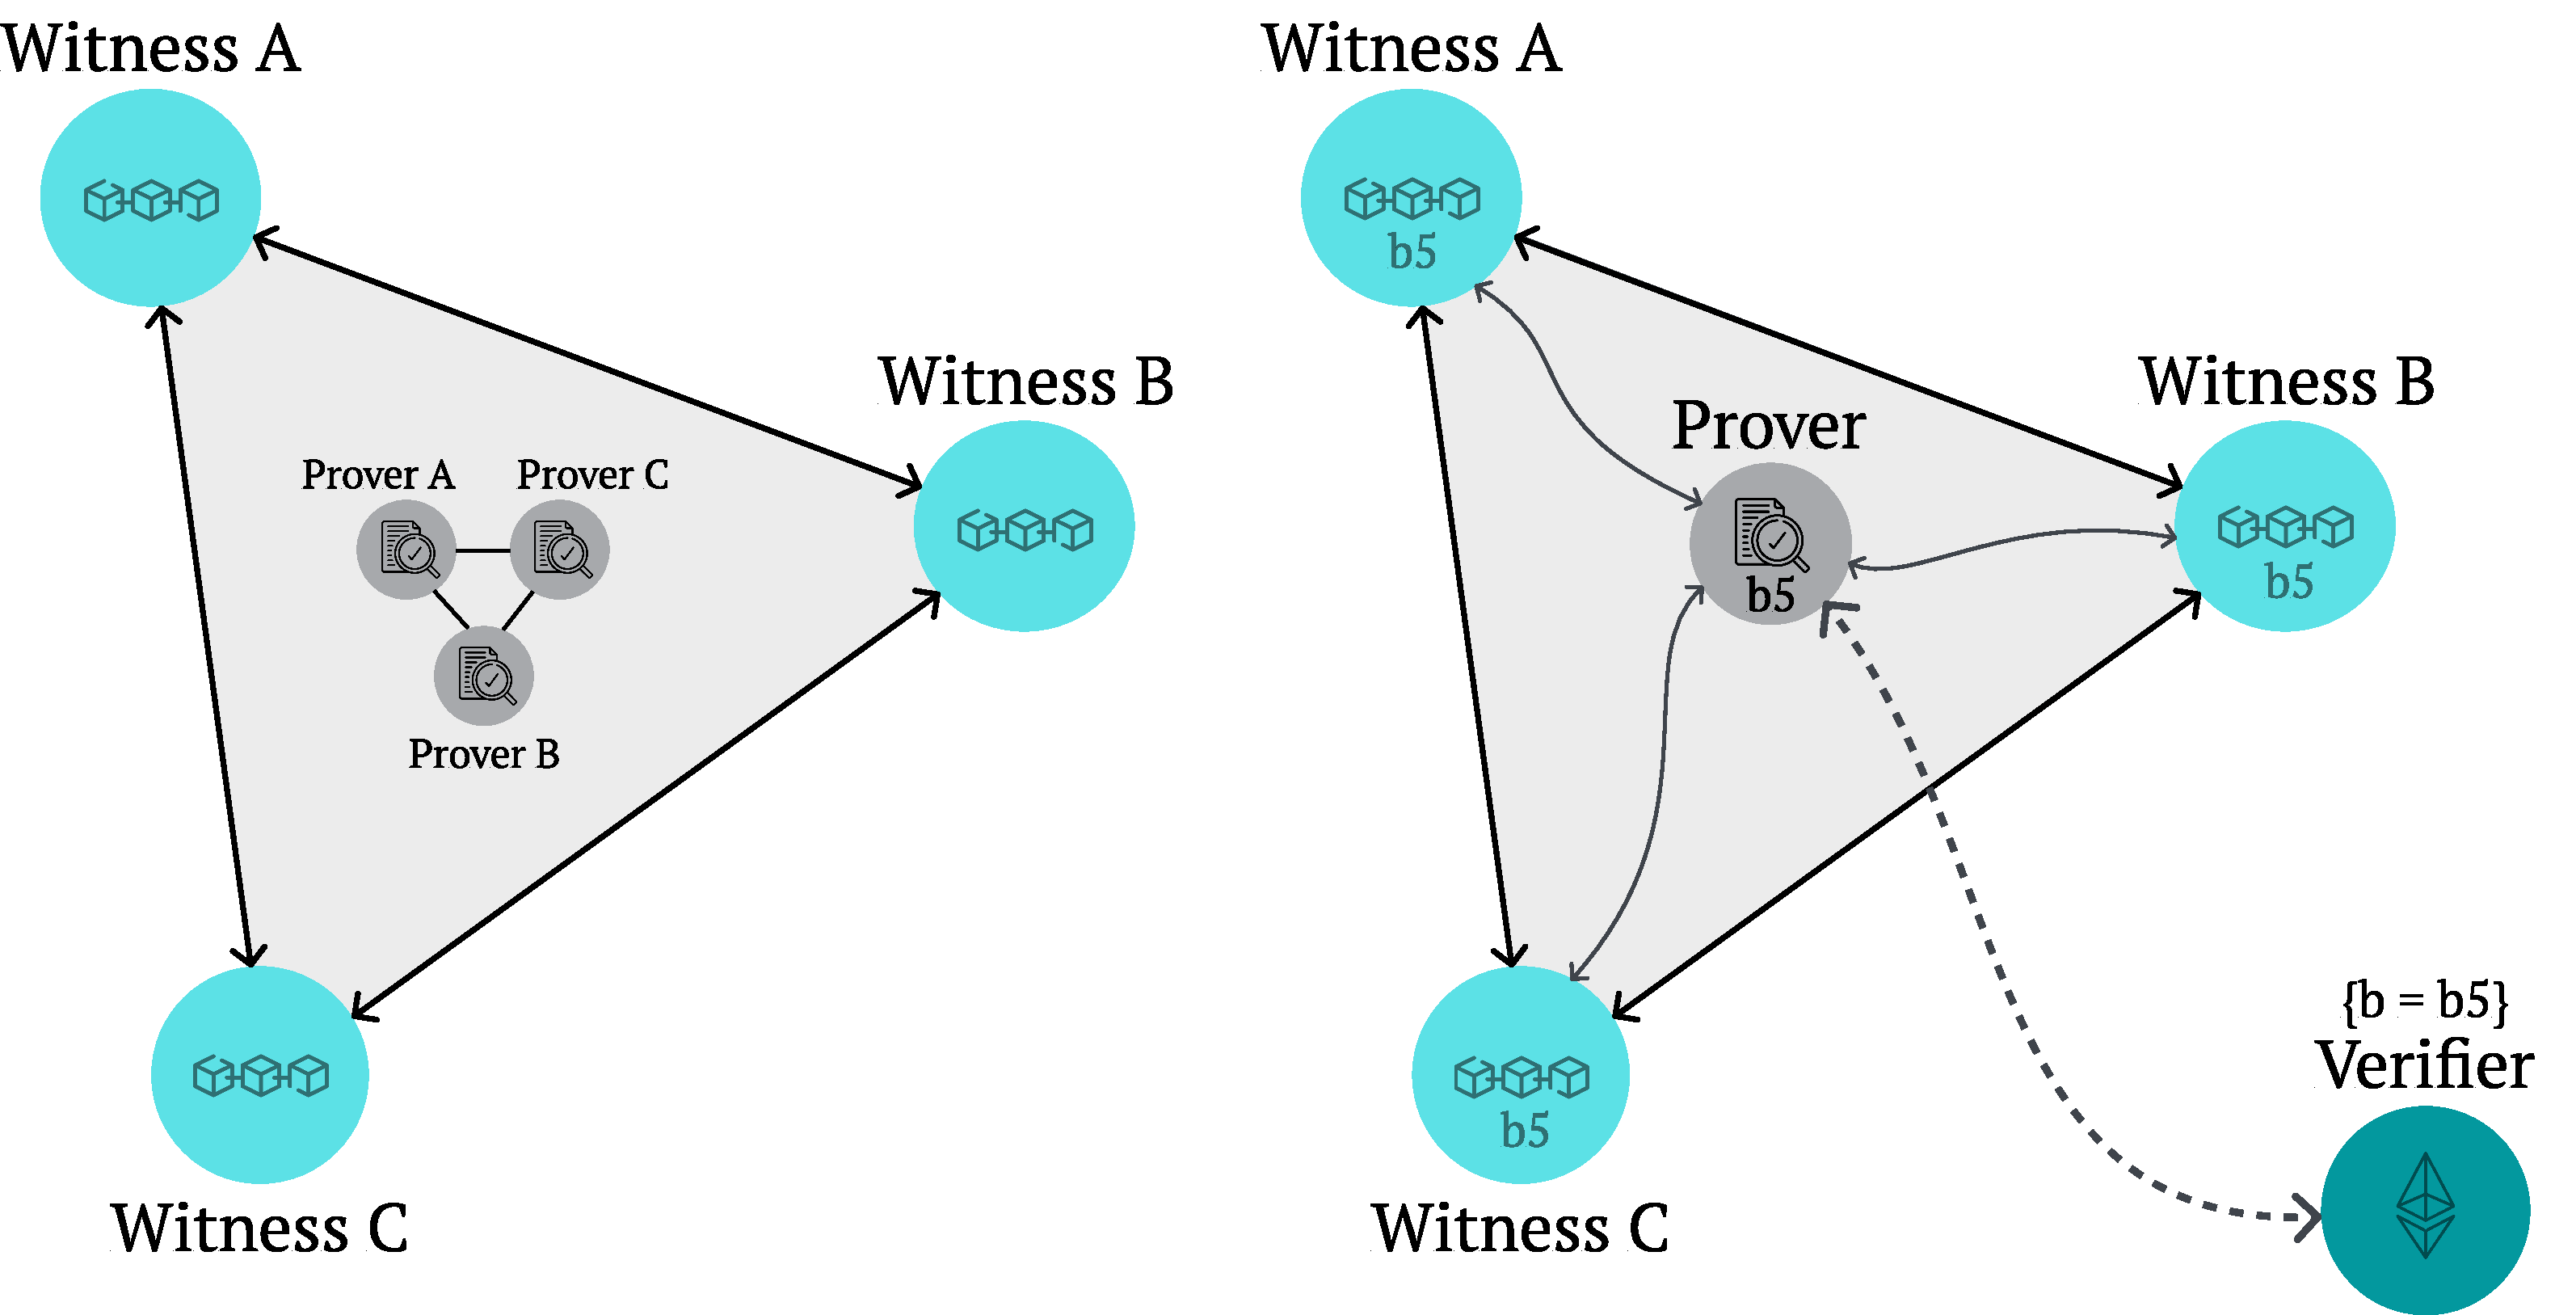
\includegraphics[width=0.9\textwidth]{overview-pol-turing.pdf}
    \caption{Some more sophisticated use cases of a Turing Complete \pol{} protocol, where the execution of zone-relative smart contracts is enabled. On the left, a multi-prover configuration, and on the right, the case where a verifier enforces the attestation of the prover's location at a specific block or time.}
    \vspace{-0.5cm}
    \label{fig:proof-of-location-overview-turing}
    \end{center}
\end{figure}

With all the above considerations in mind, this thesis is set to demonstrate the simplest case of the application of a consensus mechanism to achieve time synchronization. The goal is to experimentally prove that the block interval of a consensus mechanism can be used to synchronize  the clocks of a network of nodes, and thus, achieve zone-relative time consciousness. All the other considerations, like the extensibility of the proposed approach, the possibility of achieving a more accurate location attestation, or making use of the Turing Completeness of the system for more complex logic, are left for future work. The next section will cover the proof generation process to finally produce a \pol{} claim.

\subsection{Relative \pol{}} \label{sec:protocol-fundamentals-rel-pol}

With the witnesses agreeing on a location, short-range communication, and internal clock synchronization, the infrastructure is ready to generate a verifiable \pol{} certificate. This section will provide a description of the certificate generation process, its requirements, and a possible verification procedure that is derived from the protocol's design. 

Building upon the steps achieved in the previous sections, it is assumed that a zone has been established, and that the zone members are able to achieve time-conscious consensus. Concretely, we assume that both the prover and the witnesses restrict their communications to the zone's physical boundaries, dictated by the coverage of their short-ranged communication means, and we also assume that the zone members are able to achieve zone-relative time synchronization, and so, pace the events of the protocol's execution at the same rate. The next step is to establish the proof generation process, which is based on the zone's relative space and time. The main goal is to assert that the prover is at a specific location, at a specific time, relative to the witnesses. This means, in practical terms, that the prover is able to communicate, via the same short-ranged communication means, with all the witnesses, and is able to demonstrate that it is, as well, synchronized with their internal clocks. However, before asserting such propositions, we also assume that every entity $i$ has a unique key pair, composed of a public key $K^{pu}_i$ and a private key $K^{pr}_i$. The public key represents the identity of an entity, and is used to verify the signature of the messages produced. The private key, on the other hand, is used to sign the messages. The public key of a zone member is known to all the other members, meanwhile, the private keys shall be kept secret. 

Given that the witnesses $w \in W$ are pacing the zone events, i.e., generating new blocks, in average, at every $T$ units of time, and the last block was generated at the zone-relative time $t_x$, with a block hash $h_x$, the proof generation process is as follows:

\begin{enumerate}
    \item The prover $\rho$ synchronizes itself at the zone-relative time $t_x$ and learns the hash  $h_x$ of the last block $B_{x}$.
    \item The prover $\rho$ assembles a transaction $\text{Tx}_\rho$ containing the input $h_x$.
    \item The prover $\rho$ signs the transaction $\text{Tx}_\rho$ with its private key $K^{pr}_\rho$.
    \item The prover $\rho$ broadcasts the transaction $\text{Tx}_\rho$ to the witnesses $w \in W$.
    \item The witnesses $w \in W$ verify the transaction $\text{Tx}_\rho$.
    \item The witnesses $w \in W$ assemble a block $B_{x+1}$ with hash $h_{x+1}$, at time $t_{x+1}$, containing the transaction $\text{Tx}_\rho$.
    \item The witnesses $w \in W$ sign the new block $B_{x+1}$ with their private key $K^{pr}_w$.
    \item The witnesses $w \in W$ broadcast the block $B_{x+1}$ to the entire network.
    \item The prover $\rho$ verifies the hash $h_{x+1}$, the parent hash $h_{x}$, and the signatures of the block $B_{x+1}$, and the inclusion of its transaction $\text{Tx}_\rho$, with the matching input $h_{x}$.
    \item The prover $\rho$, finally, assembles the \pol{} certificate, containing the signed block $B_{x+1}$, by the witnesses $w \in W$, and the signed transaction $\text{Tx}_\rho$, by the prover $\rho$ itself.
\end{enumerate}

Having obtained a valid \pol{} certificate, as the prover $\rho$ was spatially synchronized with the witnesses $w \in W$ around the zone-relative time $t_{x+1}$, the next step would be to submit the certificate to a verification process. Without any verifier-specific information, the verification process would be identical to step 9 of the above procedure. Assuming that the verifier knows the identities of all the entities involved in the proof generation process, the verification process would go around verifying the signatures of both the block $B_{x+1}$ and the transaction $\text{Tx}_\rho$, by the witnesses and the prover, respectively, and verifying, as well, that the transaction input matches the parent hash $h_{x}$ of the block. This last verification step ensures that the prover was spatially synchronized with the witnesses around the zone-relative time $t_{x+1}$. A more well-founded analysis of the robustness, security, privacy, and, eventually, the correctness of this \pol{} protocol, inspired by the works presented in Chapter~\ref{sec:related-work}, is left for future work. This would, as well, include a more detailed analysis of the security against the most common attacks and collusion scenarios, like proxy attacks or witness collusions. Bridging with the examples presented in Figure~\ref{fig:proof-of-location-example-scenarios}, in the first use case, the prover is represented by the reporter, and the witnesses are the bystanders that are passing by the accident site. The goal of the reporter is to prove that he was physically present at the location of the accident, factually covering the event. The proof, possibly containing a piece of media content, is attested by the onlookers and verified by a journalist when producing a news piece. In the second case, the ISP assumes the prover role and tries to gather a proof of the service provision within the customers' neighbourhood. Ultimately, the proof can be verified by regulators that are responsible for the enforcement of service level agreements.

\newpage  

\begin{figure}[h!]
    \begin{center}
    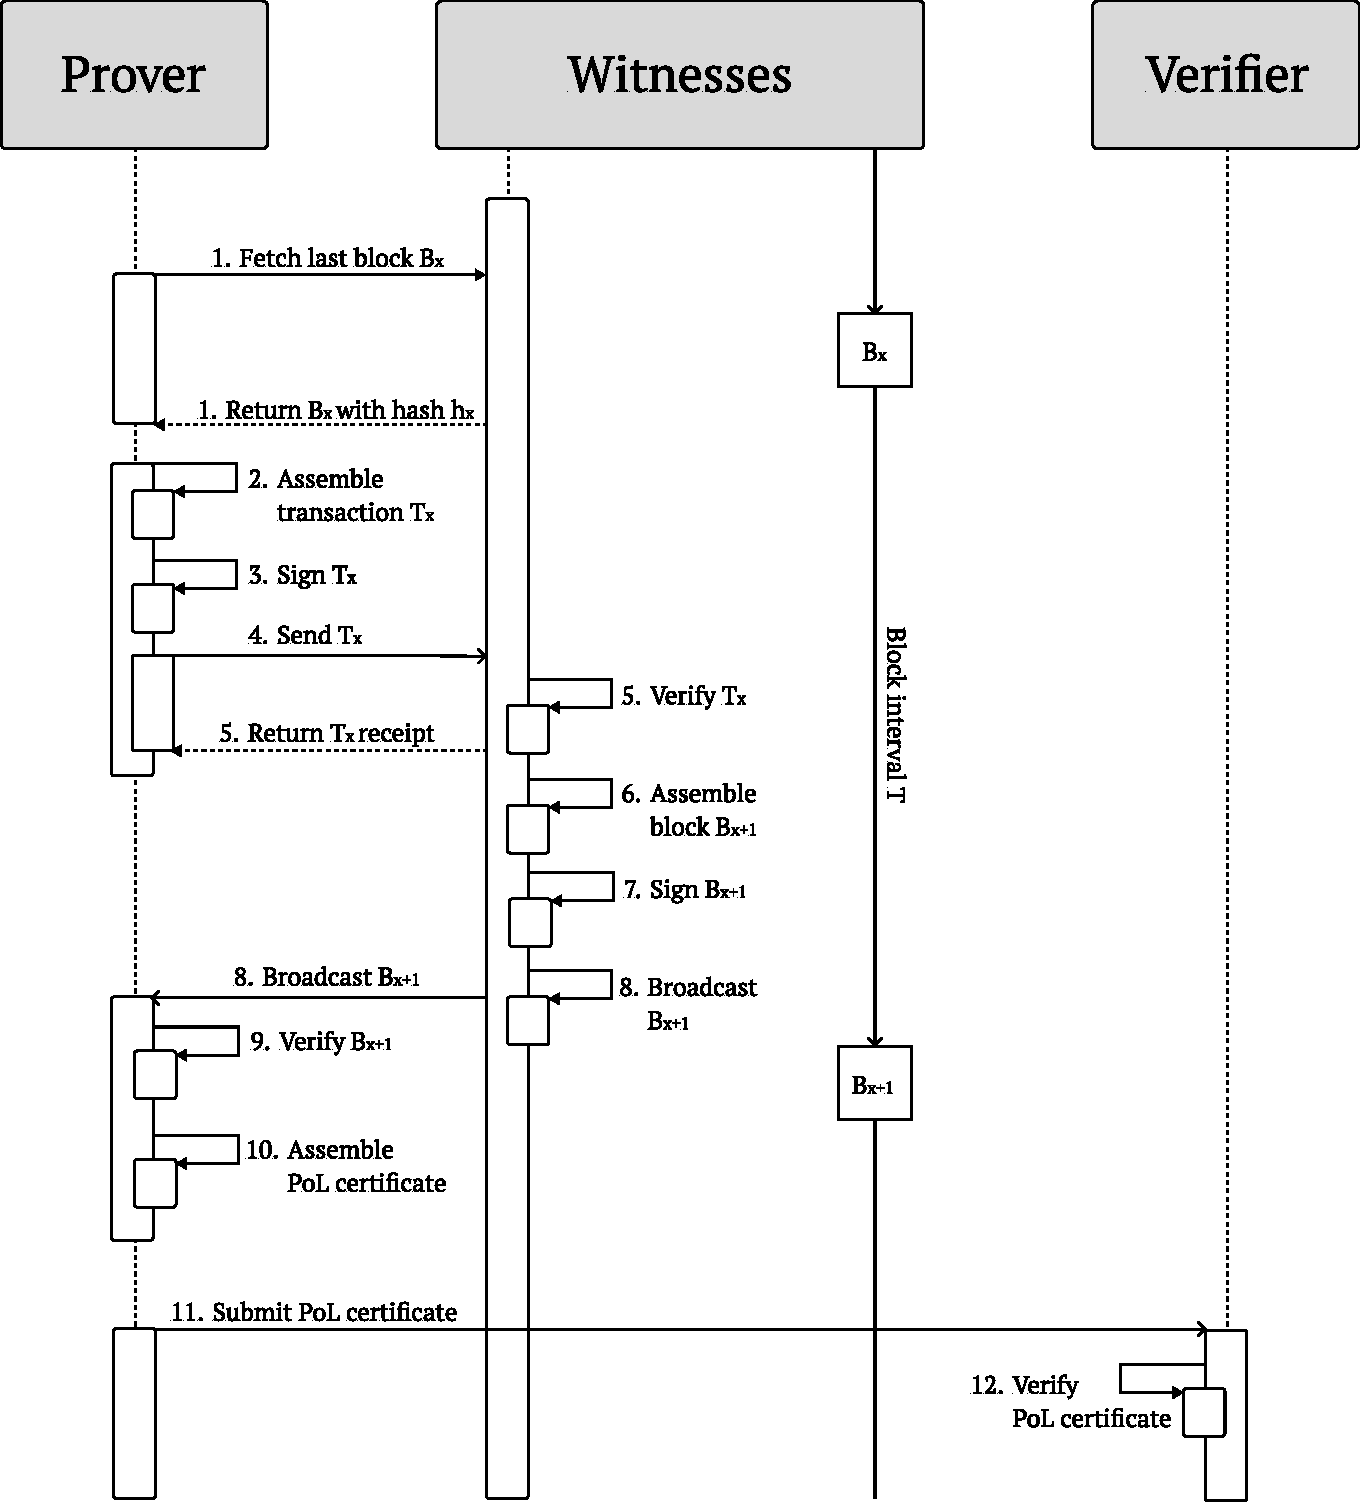
\includegraphics[width=\textwidth]{overview-pol-rel-seq.pdf}
    \caption{Sequence diagram overview of the proof generation process.}
    \vspace{-0.5cm}
    \label{fig:proof-of-location-overview-relative-pol-seq}
    \end{center}
\end{figure}

Up to this point, the protocol has been described in a relative manner, i.e., the prover is able to prove its location relative to the witnesses. The underlying mesh network enabled the short-ranged communication, while a permissionless consensus mechanism allowed for the time synchronization and generation of a verifiable certificate. The next section will provide a rough outline of how this protocol can be extended to achieve Absolute \pol{}, involving the introduction of verified space and time references.

\subsection{Absolute \pol{}} \label{sec:protocol-fundamentals-abs-pol}

Having established a means for Relative \pol{}, ensuring space and time synchronization within a zone, the next step would be to extend the protocol to finally achieve Absolute \pol{}. A possible path consists in combining the procedure with a Global Time Synchronization Protocol and a Global Positioning System, as illustrated in Figure~\ref{fig:proof-of-location-overview-absolute-pol}.

\begin{figure}[h!]
    \begin{center}
    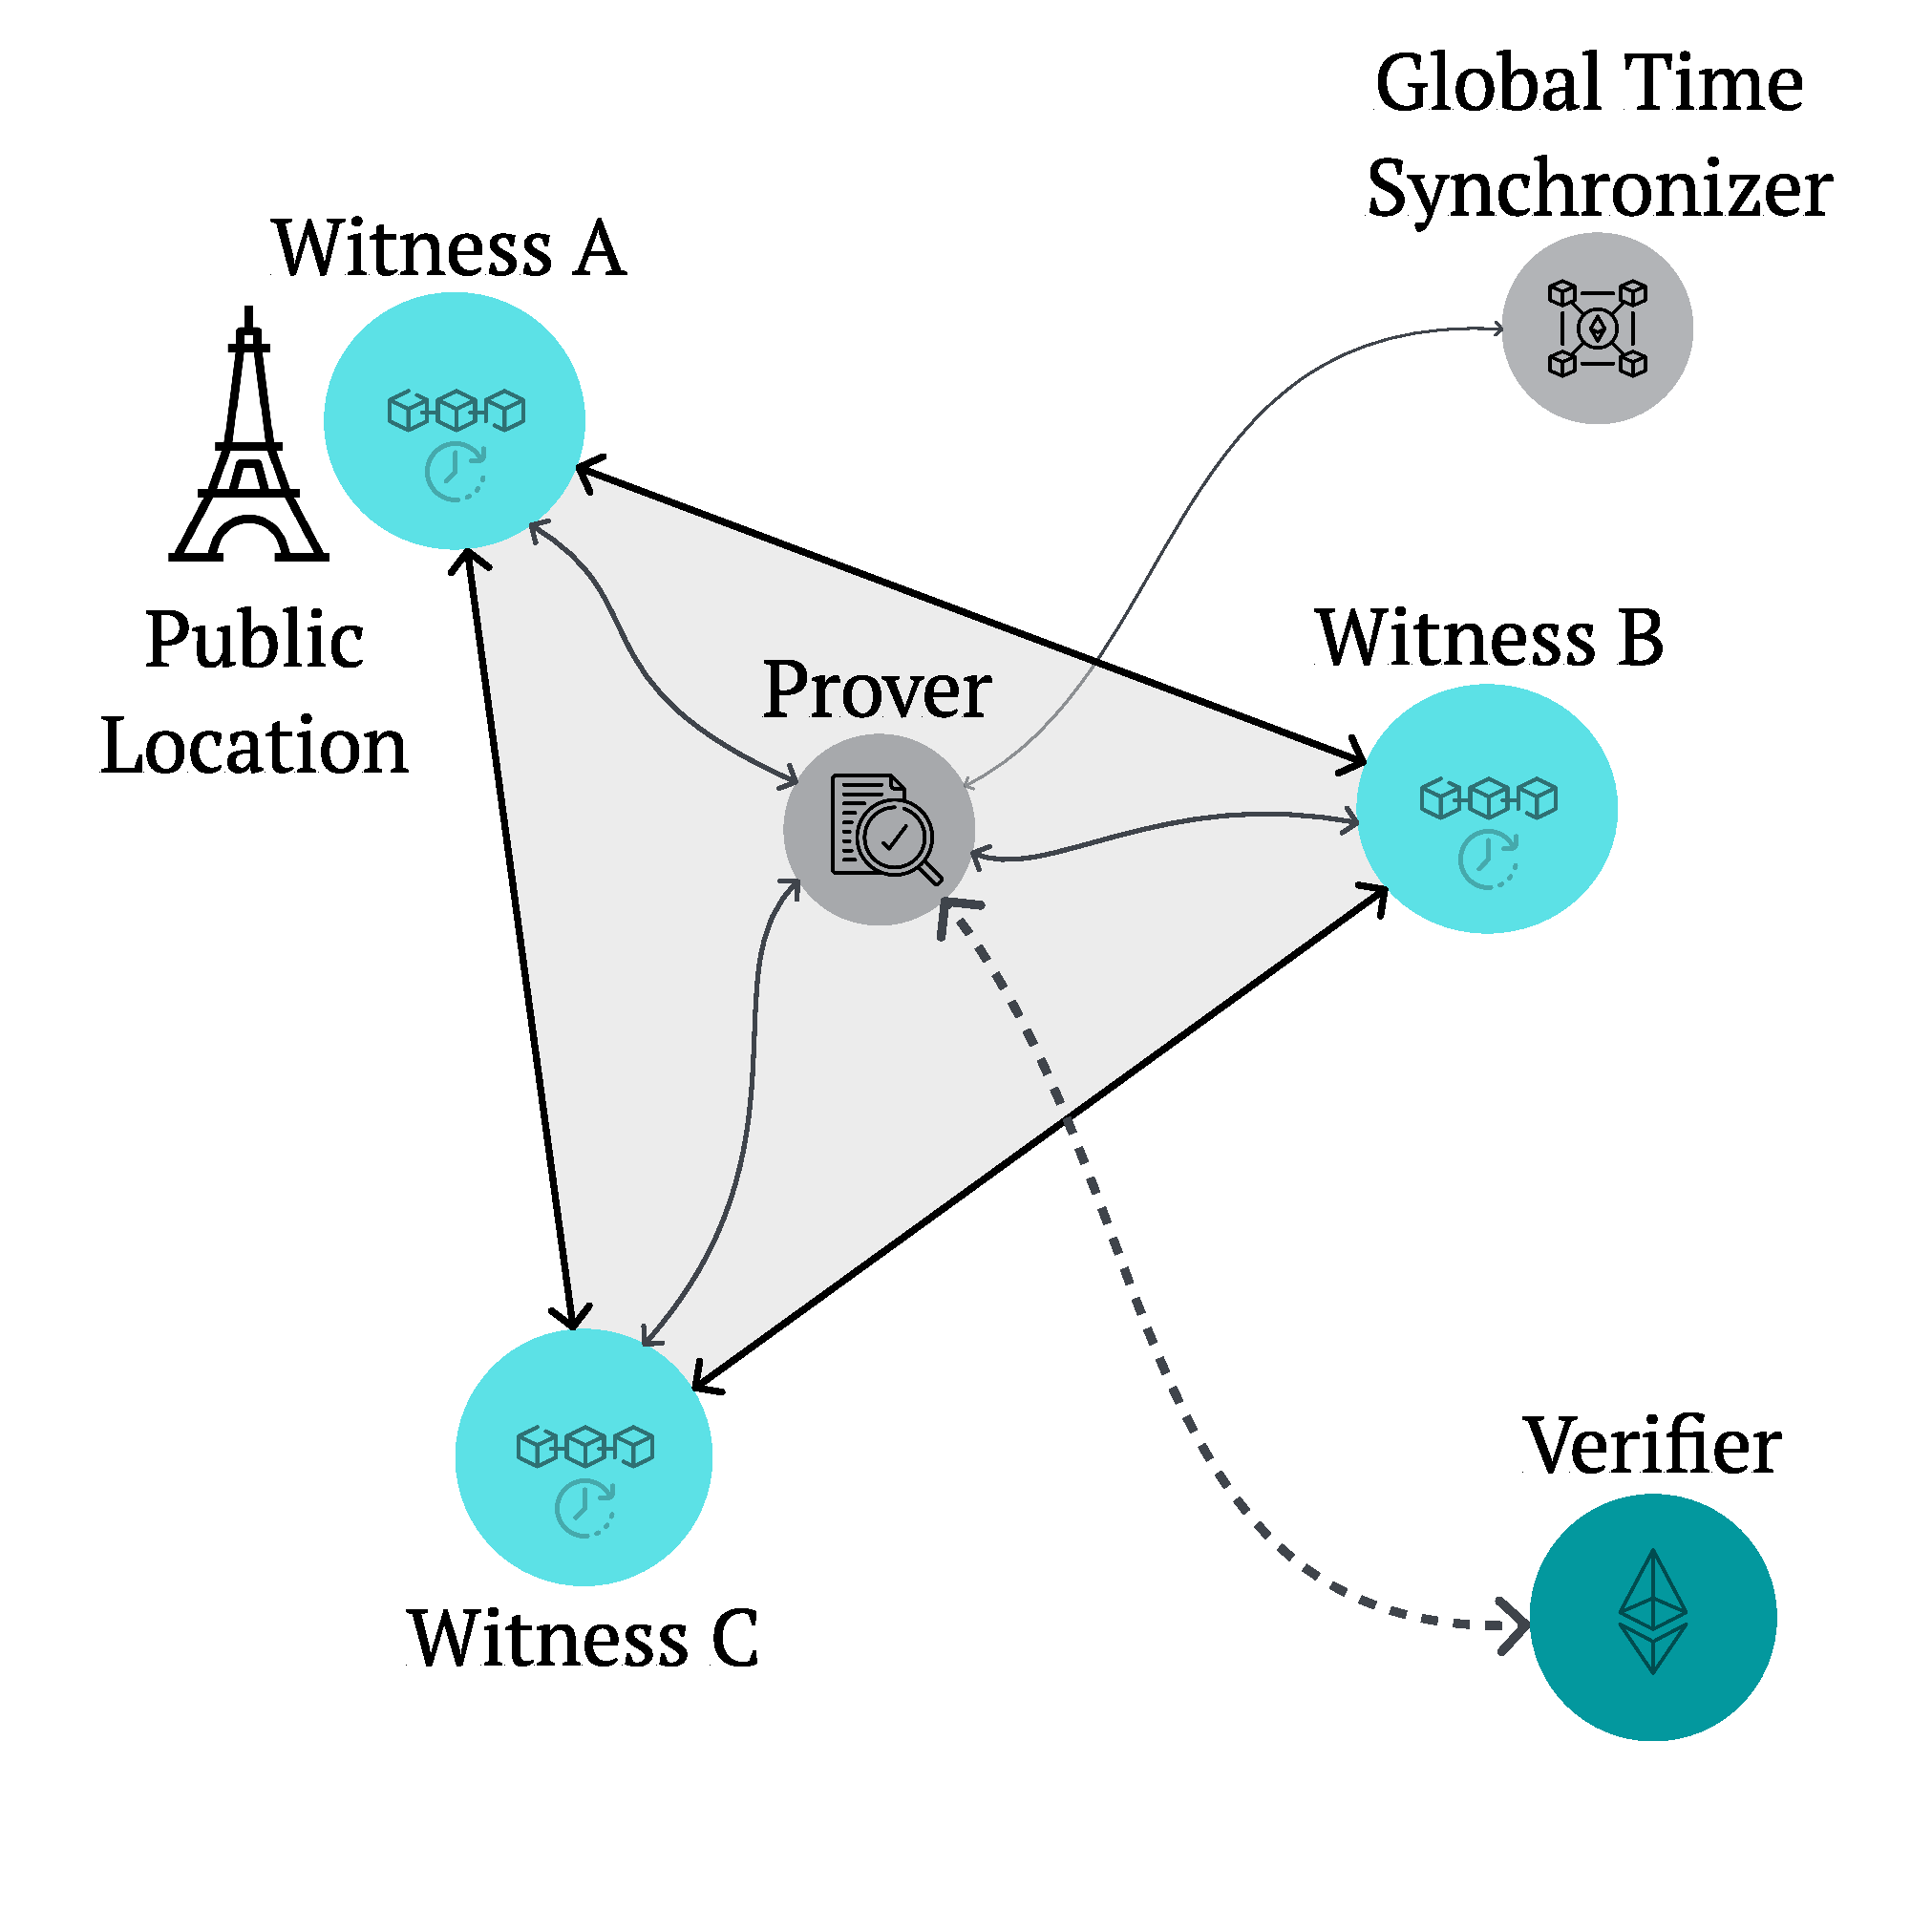
\includegraphics[width=0.55\textwidth]{overview-pol-abs-pol.pdf}
    \caption{Achieving Absolute \pol{} by combining Relative \pol{} with a Global Time Synchronization Protocol and a Global Positioning System.}
    \label{fig:proof-of-location-overview-absolute-pol}
    \end{center}
\end{figure}

The goal is to produce a \pol{} certificate that is spatio-temporally sound, relative to the zone, but which can, as well, be spatially and temporally acknowledged by any other node outside the zone. This effort may require, for instance, a global timestamping server, or protocol that can assert a certain level of globally secure timestamp accuracy in a tamper-proof manner. In a decentralized fashion, one example of such a system is a public Blockchain network, such as Bitcoin \cite{nakamoto2008bitcoin}, or Ethereum \cite{buterin2014next}. The same applies to the Global Positioning System (GPS). A standard system of geographic coordinates could be validated and embedded into the \pol{} certificate, to globally assert the location of the whole zone \cite{amoretti2018blockchain ,nosouhi2020blockchain}. It is worth noting that the Relative \pol{} protocol is flexible enough to accommodate any kind of higher level protocol, including more complex certificate formats, tighter trust levels, and composite information to be signed. This and further extensions are left for future work. \\

This chapter has laid the path towards a decentralized \pol{} protocol. We have started by proposing a mesh network topology to provide a decentralized and self-organizing network infrastructure. This underlying arrangement of nodes enables peer-to-peer and short-range communication, which is essential for the soundness of the protocol. Next, we have proposed a new way of synchronizing the internal clocks of trustless witnesses. This approach takes advantage of permissionless consensus mechanisms to establish zone-relative time consciousness and simultaneously enable the serialization of events in a tamper-proof manner. We have also considered the choice of a Turing-complete consensus system to allow for the decentralized execution of computations and deployment of zone-relative location services. Finally, we have proposed a \pol{} protocol that can produce a verifiable and spatio-temporally sound location certificate, relative to a zone. From Relative \pol{}, we are concluding the chapter with some thoughts on extending the protocol to achieve Absolute \pol{}.


\newpage
\section{Proof-of-Concept} \label{sec:proof-of-concept}

This chapter details the steps taken to develop and evaluate the \poc{} implementation. Section~\ref{sec:proof-of-concept-infrastructure} provides an overview of the infrastructure, while Section~\ref{sec:proof-of-concept-pol-implementation} describes the implementation of the \pol{} protocol, after the establishment of the baseline network architecture. Finally, Section~\ref{sec:proof-of-concept-results} presents some measurements of the \poc{} evaluation. All the software developed, along with complementing documentation, is available at the repository referenced in Appendix~\ref{appendix:repository}.


\subsection{Infrastructure} \label{sec:proof-of-concept-infrastructure}

Aiming at meeting the requirements established in Chapter~\ref{sec:protocol-fundamentals}, the system design process and infrastructure choices for accomplishing the establishment of a mesh network were crucial in ensuring its operability. The following sections describe the design of the system and the testbed setup, as well as the challenges faced during the establishment of the network infrastructure.

\subsubsection{System Design} \label{sec:infrastructure}

One of the critical decisions was the selection of an appropriate operating system (OS) for configuring and enabling an ad hoc and dynamic mesh network. Multiple Linux distributions were initially explored, including OpenWrt, Raspbian, and Ubuntu. After careful consideration and a handful of failed attempts, OpenWrt led the track to host the protocol implementation. Its automated build tools and configurable packages, including the straightforward B.A.T.M.A.N. kernel module integration, load, and setup, made it a suitable choice for the flexible customization of the mesh network. The OS's active development community and extensive documentation further supported its use. As mentioned in Section~\ref{sec:background-wireless-mesh-networks}, OpenWrt is a lightweight solution for embedded devices, supporting a considerable set of platforms and toolchains for targeted integration of embedded software. Its choice turned out to be strategic regarding as well the role played in the spawning of decentralized and community-driven computer networks, that actively contribute to and are powered by such open source projects, all around the world\footnote{\url{https://en.wikipedia.org/w/index.php?title=Freifunk}}.

The OpenWrt image building process took advantage of the official Image Builder pre-compiled environment in order to create a custom image, skipping the need for source compilation\footnote{\url{https://openwrt.org/docs/guide-user/additional-software/imagebuilder}}. The process was automated with the help of a \emph{Dockerfile}, not only to allow for an easy integration and further testing of the mesh network pre-compiled packages, but also to enable the experimentation with different network settings and the quick embedding and deployment of the \pol{} protocol software. The Image Builder setup is located under the "proof-of-concept/openwrt-builder" directory of the thesis repository. The packages were chosen to provide deployment and debugging support for mesh networking using \emph{batman-adv}, wireless security using WPA/WPA2, working with the \emph{ext4} file system, and interacting with an Ethereum network via the official \emph{geth} client. The images were experimentally compiled for \emph{x86-64}, \emph{bcm2708}, and \emph{bcm2709} targets, being the last two ideal for the Raspberry Pi Zero and Raspberry Pi 2/3/4 models, respectively\footnote{\url{https://firmware-selector.openwrt.org/}}.

\subsubsection{Testbed Setup} \label{sec:infrastructure:testbed}

% Raspberry Pi failure deploymment
% Choice for QEMU for ease of testing and deployment
% Description of the testbed, including the hardware emulated, characteristics, etc.
% Description of the tap and bridge interfaces, etc.

The next step was to set up a testing environment for the deployment and running of the \pol{} protocol. Up to the delivery of this thesis, efforts are being made to port the generated OpenWrt image and compiled protocol modules to physical Raspberry Pis. However, the deployment on physical devices and the configuration of wireless interfaces is proving to be a challenge on multiple levels. The current drawbacks we are facing relate to the automated enabling of the batman-adv network interface, in order to allow for the autonomous start of a dynamic and ad hoc mesh network. Nevertheless, even when manually configuring the interfaces, the protocol process of dynamic neighbourhood discovery is also failing, as the wireless interfaces are not able to easily detect each other, or establish a stable connection. We have been further investigating these issues to identify the root cause of these problems, and to finally uncover the solution for the deployment on physical devices. These attempts and the physical demonstration of the \pol{} protocol are set for future work.

Meanwhile, to ease such development and testing hustle and to allow for a more flexible and faster deployment of the protocol, we have set up a virtualized environment, using QEMU (see Section~\ref{sec:background-wireless-mesh-networks}). The environment was configured to emulate a set of x86-64 target devices, and to run the OpenWrt image with the embedded and target-compiled \pol{} software. The testbed setup followed the guidelines of the official batman-adv documentation\footnote{\url{https://www.open-mesh.org/doc/devtools/Emulation_Environment.html}}, and the source code is available under the "proof-of-concept/qemu" directory. To reduce manual input, an automated script was programmed, expecting the previously built OpenWrt image, and defining variables for the instance type, either “witness” or “prover”, the instance number, and a GDB port, for kernel debugging. The script creates a shared bridge for the cluster and a unique tap interface for each virtual machine, assigning to them an individual MAC address. Finally, the script launches QEMU by creating a new virtual disk image, as a copy-on-write snapshot of OpenWrt, and by setting up each virtual machine with 1 GB of memory, 2 virtual CPUs, and a virtual SCSI disk. It assigns, as well, internal network interfaces to the instances. One uses the previously created tap interface to flush the mesh network traffic, and a second one is a virtual NIC to allow for the usual internet connection\footnote{\url{https://www.open-mesh.org/doc/devtools/OpenWrt_in_QEMU.html}}. KVM is also enabled, in order to speed up the emulation, as well as a virtual RNG (Random Number Generator) and a virtual serial port. Up and running, with three witnesses and a prover instance, the testbed looks as depicted in Figure~\ref{fig:infrastructure:testbed}.

\begin{figure}[h!]
    \begin{center}
    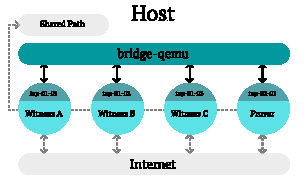
\includegraphics[width=0.9\textwidth]{proof-of-concept-qemu.pdf}
    \caption{Testbed setup for the \pol{} protocol.}
    \label{fig:infrastructure:testbed}
    \end{center}
\end{figure}

\subsubsection{Network Architecture} \label{sec:infrastructure:network-architecture}

After the establishment of the testbed, the physical networking layer is emulated by the bridge interface, which is set to pool all the mesh traffic that flows into and from the tap interfaces. The step that follows is the configuration of the batman-adv kernel module, responsible for the dynamic and ad hoc mesh network creation. This step was automated at the OpenWrt image building process, with the inclusion of custom instructions in the image startup scripts. These instructions set the routing algorithm and enable the virtual Ethernet interface eth0, linking the tap interface created before to the batman-adv interface bat0. The interval time between the broadcasting of neighbourhood discovery messages is set to 5 seconds, which determines how often a node should broadcast its presence in the network. The bridge loop avoidance mechanism is activated, penalizing the routing of traffic through routes with more hops. This last step is important to avoid the creation of loops in the network and to ensure the traffic is always routed through the shortest path, forcing the nodes to communicate directly with each other, within the testbed. Finally, the script disables the firewall to avoid any interference with batman-adv, and flushes the IP addresses of both the eth0 and bat0 interfaces.

Subnetting is then done via the assignment of an IP address to the bat0 interface. The IP address of each instance is generated based on the MAC address of eth0, establishing a non-conflicting address in the 192.168.0.x/24 subnet. After this step, the network is ready to use the TCP/IP stack, and the \pol{} protocol can be deployed, configured, and run. The final network topology is depicted in Figure~\ref{fig:infrastructure:network-architecture}.

\begin{figure}[h!]
    \begin{center}
    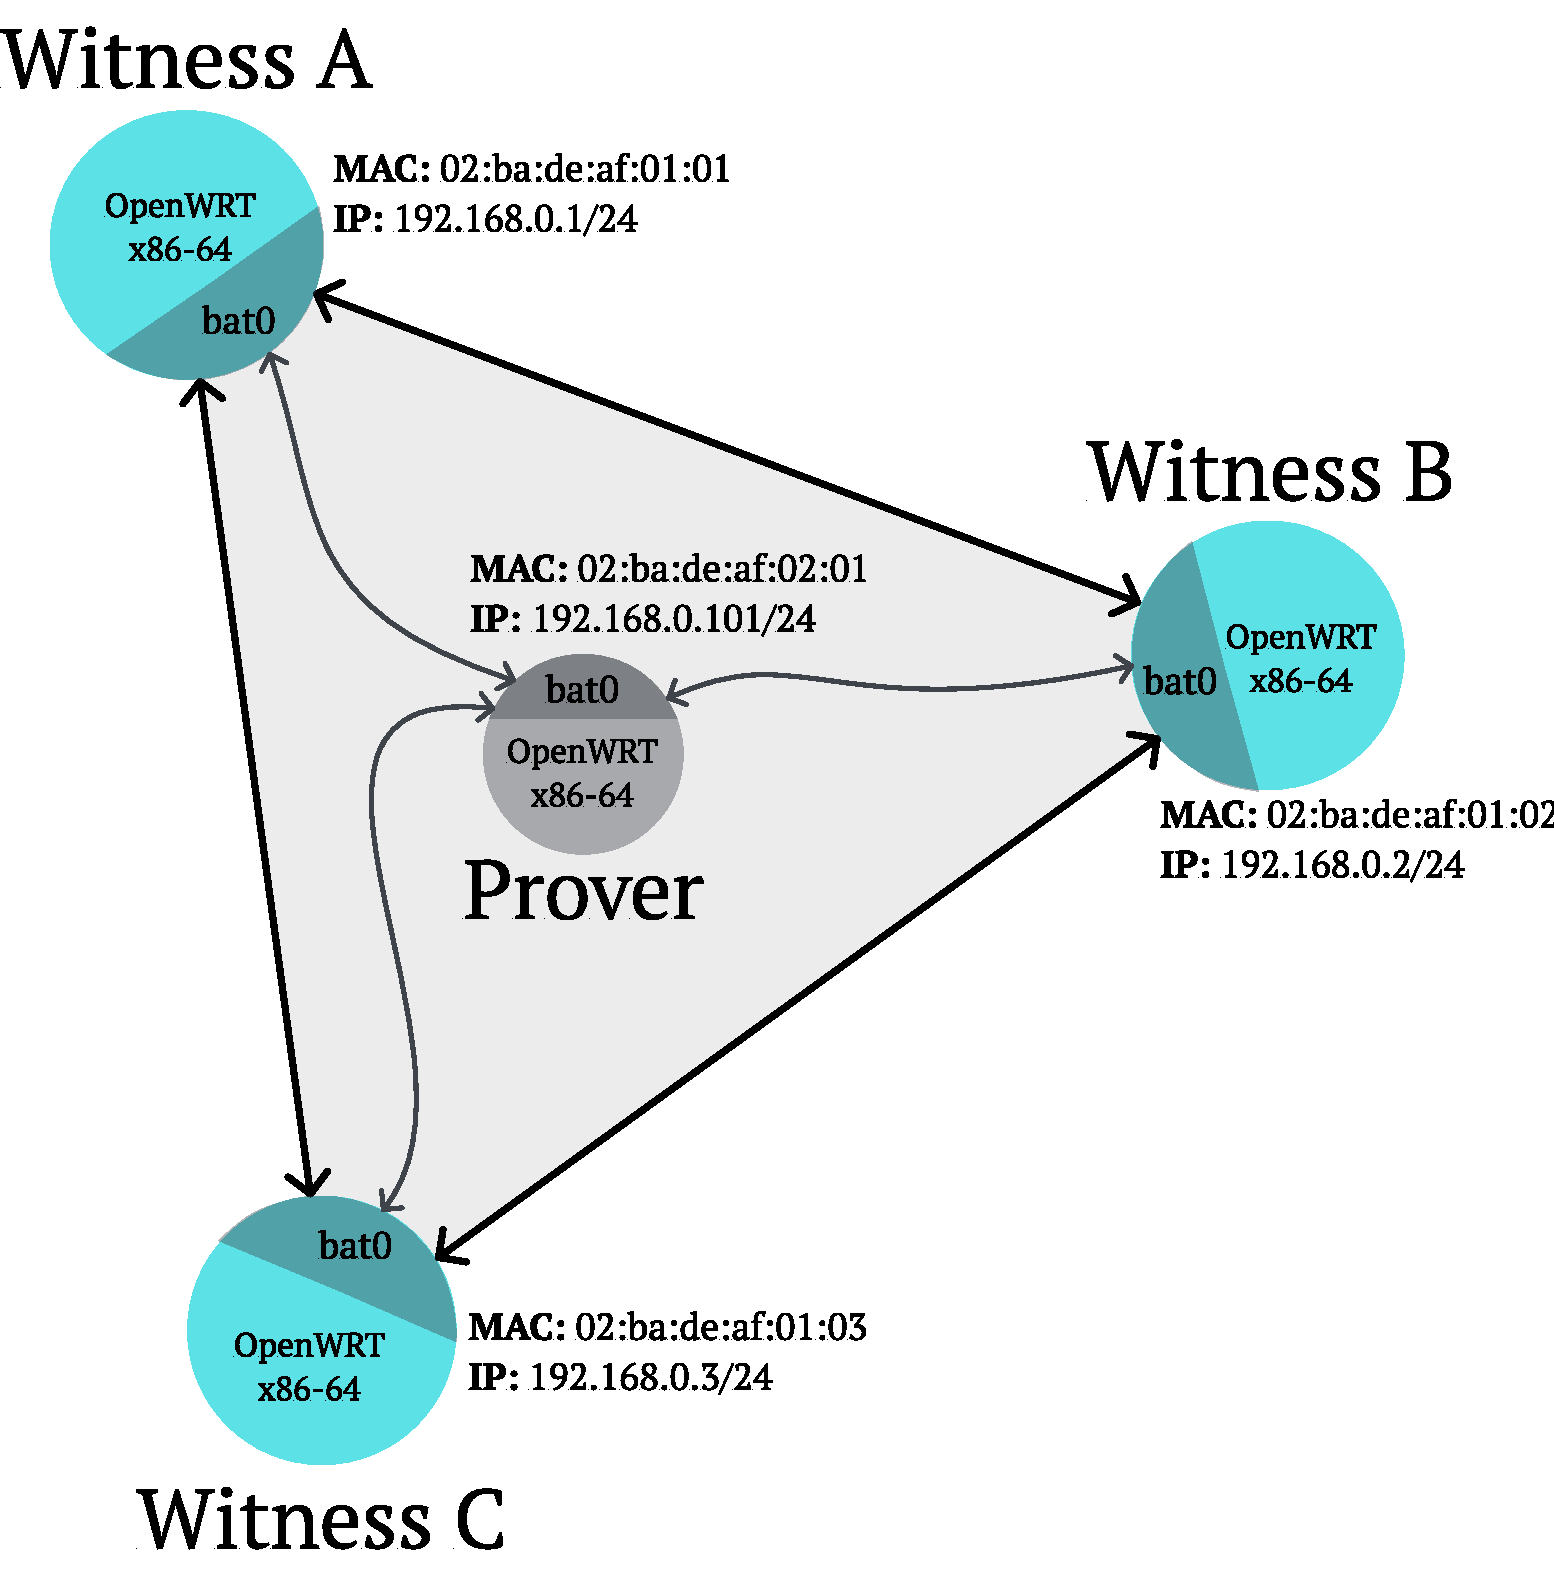
\includegraphics[width=0.7\textwidth]{proof-of-concept-network-topology.pdf}
    \caption{Network topology of the system under test, after configuring the batman-adv interface and assigning IP addresses to the instances.}
    \label{fig:infrastructure:network-architecture}
    \end{center}
\end{figure}

\subsection{Protocol Implementation} \label{sec:proof-of-concept-pol-implementation}

The steps above ensured the establishment of the physical, data link, network, and transport layers, drawing up the foundation for the application layer, featuring the actual implementation of the \pol{} protocol. In this section, we provide a description of the protocol setup, including the reasoning and choice for the Blockchain framework to use. The processes of proof generation and verification are also detailed.

\subsubsection{Practical Permissionless Consensus} \label{sec:pol-implementation:practical-permissionless-consensus}

The outline provided in Section~\ref{sec:protocol-fundamentals-clock} identified the need for a clock synchronization mechanism that would finally enable spatio-temporal soundness. Space synchrony is achieved with the assumptions around the short-ranged communication means. Time synchrony, on the other hand, is achieved with a clock synchronization mechanism. The hypothesis involved the employment of a permissionless consensus protocol to establish zone-relative time consciousness, but with the added benefit of providing strongly consistent serialization of transactions and total order of multidimensional events, instead of simply counting time in a unidimensional manner, via a plain clock synchronization protocol. The practicalities of employing a permissionless consensus mechanism involved the experimentation with a blockchain framework, the deployment of an interacting client, and the setup of the network.

The beginning of the exploration process included the prototyping of an ad hoc Proof-of-Work based consensus protocol, to assess the feasibility of the hypothesis. This work was part of the 2022 Fall Semester's edition of the Distributed Systems seminar, where an analytical approach was taken to survey multiple permissionless consensus mechanisms, pointing out the challenges of porting such protocols to resource constrained environments\footnote{\url{https://github.com/edurbrito/dist-sys-seminar}}. The results of the experiment were sufficiently encouraging to warrant the development or choice of a more robust and scalable implementation. Multiple open source projects were considered, and the ultimate decision relied on Ethereum and its flexible tooling for creating private networks\footnote{\url{https://geth.ethereum.org/docs/fundamentals/private-network}}. Initially, the successful attempts at interacting with Ethereum concealed a handful of problems that would be later exposed. The smart contracts' functionality, for instance, was presenting issues at the execution and output conversion. The problems were ultimately traced back to the use of a different version of the contract's compiler, which was not compatible with the version of the client used. Some of the issues persisted, which led us to ask for help from the Ethereum community, in GitHub\footnote{\url{https://github.com/ethereum/go-ethereum/issues/27009}}, StackExchange, and other forums. We have eventually solved the problem, with a custom compilation of the software, and have successfully blended its official client implementation, \emph{geth}, into the OpenWrt image.

The prerequisites for the establishment of an ad hoc Ethereum network expect first the configuration of a \emph{Genesis} file and a local data directory, to set the initial state of the network and progressively save the history, as the blocks get mined. Configuring the genesis block resorts, as well, to the choice of a consensus protocol. The geth client supports two main consensus protocols, a Proof-of-Work (PoW) and a Proof-of-Authority (PoA) based mechanism. Both protocols were tried out, but PoA was ultimately chosen for carrying out the remaining tests, since it offered a more controlled environment for the flexible adjustment of multiple parameters, like the block time. A more thorough analysis of the PoW and PoA protocols, as well as trade-offs and performance comparisons, are left for future work. The PoA protocol relies on a list of authorized signers, which are allowed to mine blocks \cite{clique-eth}. The signers' list is defined in the genesis block, and the private key of each signer is used to sign the blocks. We have automated the key pair generation at startup and developed multiple utility programs to facilitate the deployment of the nodes and the execution of the protocol. These custom tools were written in Golang and compiled for the target platform, to be used as part of the OpenWrt image, serving also as demonstration of the feasibility of the process of embedding custom software into the system. These command-line programs can be found under the "proof-of-concept/src/geth-utils" directory. Among other tasks, they automate the initialization of the blockchain nodes, via the genesis file, and the establishment of the network, via the discovery of bootnodes and connection of new peers. Each node exposes the necessary API endpoints to allow for the interaction with the rest of the protocol participants. Network rules were also configured to restrict the communication to the zone subnet, as well as a caching policy to avoid unnecessary resource consumption. Everything was accomplished with the help of the Ethereum geth client, and the final blockchain network arrangement is illustrated in Figure~\ref{fig:pol-implementation:blockchain-network}.

\begin{figure}[h!]
    \begin{center}
    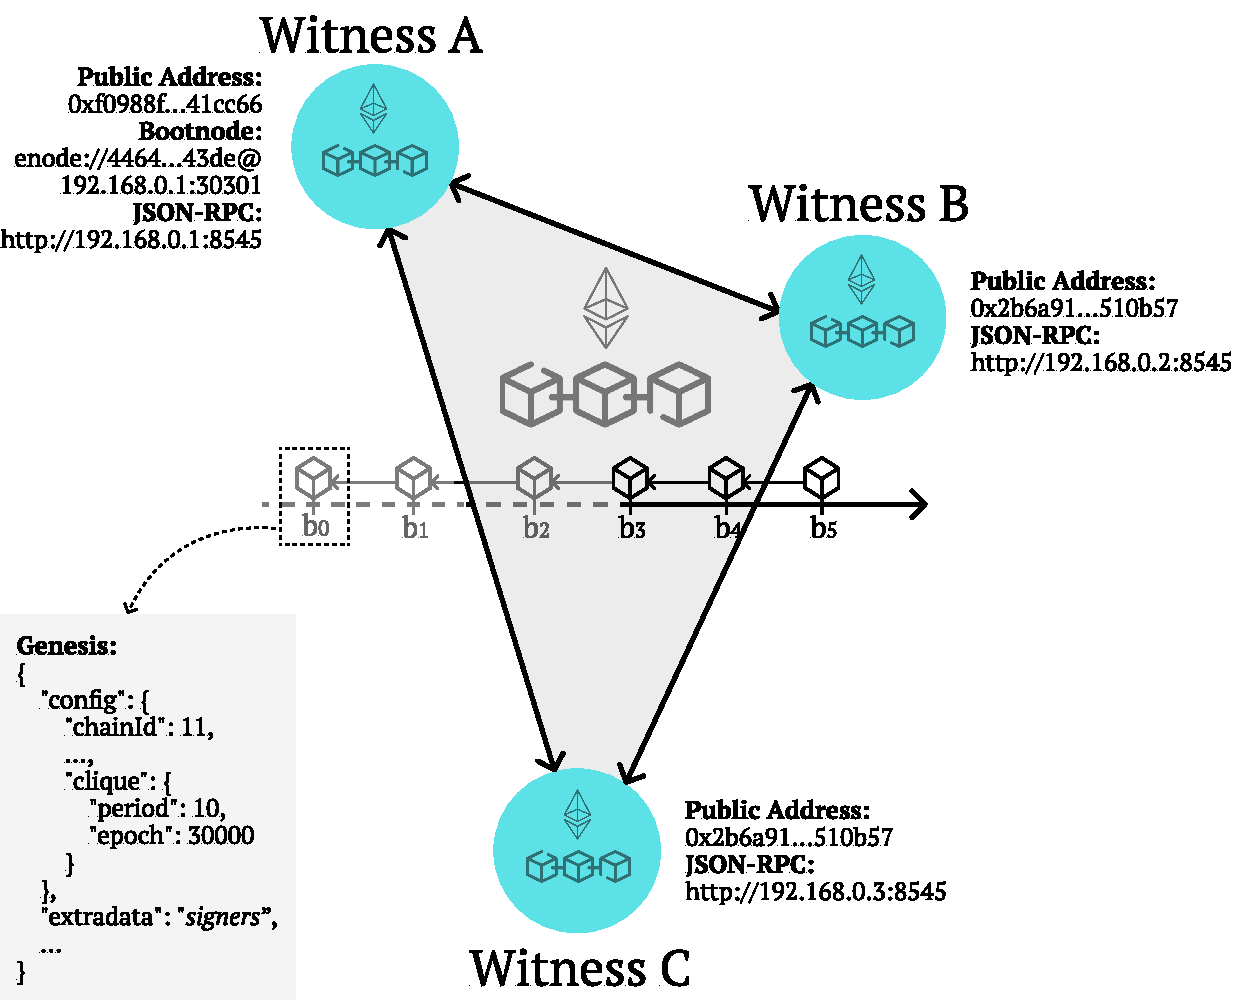
\includegraphics[width=0.75\textwidth]{proof-of-concept-blockchain.pdf}
    \caption{The Ethereum blockchain network setup, featuring a Proof-of-Authority consensus protocol with a block time of 10 seconds.}
    \label{fig:pol-implementation:blockchain-network}
    \end{center}
\end{figure}

\subsubsection{Proof Generation and Verification} \label{sec:pol-implementation:proof-generation-verification}

Guaranteed the establishment of a permissionless consensus mechanism, the witnesses are synchronized in time. The prover can now take advantage of this synchrony to request the generation of a \pol{} certificate. To accomplish such task, the prover instance, which is also part of the mesh network communication channel and has been assigned an IP address in the same subnet, needs to interact with the running blockchain and follow the protocol specified in Section~\ref{sec:protocol-fundamentals-rel-pol}. 

The automation of the prover process was also achieved with the help of a Golang utility program, found under the "proof-of-concept/src/geth-utils" directory. The prover chooses first a random witness and inquires it about the most recent block. After that, the prover assembles, signs, and submits a transaction. All the requests are accomplished via the JSON-RPC API exposed by the geth client running in the witnesses' machines. The transaction is then broadcasted to the network and the prover waits for it to be included in a block. Once the transaction is confirmed, the prover can verify its validity. If valid, it can finally request the block signatures from the witnesses. The transaction validation process may be automated via the deployment of a smart contract in the network, decentralizing and automating the procedure. We have also developed and successfully deployed an example of a smart contract, located in the "proof-of-concept/src/block-verifier" directory. The contract was written in Solidity\footnote{\url{https://docs.soliditylang.org/en/v0.8.19/}}, compiled to the Ethereum Virtual Machine (EVM) bytecode, and included in the genesis file. It compares the input hash, submitted by the prover, with the hash of the last block in the network. The contract is invoked via a typical blockchain transaction, and returns a boolean value, indicating whether the transaction is valid or not, automating the validation process that would otherwise be performed manually, by either the prover or the verifier. This approach serves as demonstration of the feasibility of the deployment of smart contracts in the zone's blockchain. More sophisticated contracts can be developed and deployed according to application needs, expanding the possibilities of the protocol and its use cases for providing decentralized and zone-relative location services (see Section~\ref{sec:protocol-fundamentals-clock}). Furthermore, the success of the proof generation process is dependent on the adjustment of the block time, which is a parameter that can be configured in the chosen PoA protocol, via the genesis file. During the implementation, we have set the block time $T$ to 10 seconds. Similar to the time-limited approach presented by Nosouhi et al. \cite{nosouhi2020blockchain}, the block interval serves the purpose of preventing proxy or wormhole attacks, as depicted in Figure~\ref{fig:pol-implementation:overview-proxy-wormhole}, shortening the chances for an adversary that is synchronized with the witnesses to interact with a remote prover and still be able to generate a spatio-temporally sound \pol{} certificate. This time interval should be planned and adjusted according to the application needs and the desired levels of security. The next section discusses the effects of the adjustment of the block time on the protocol performance, security, and success rates.

\begin{figure}[h!]
    \begin{center}
    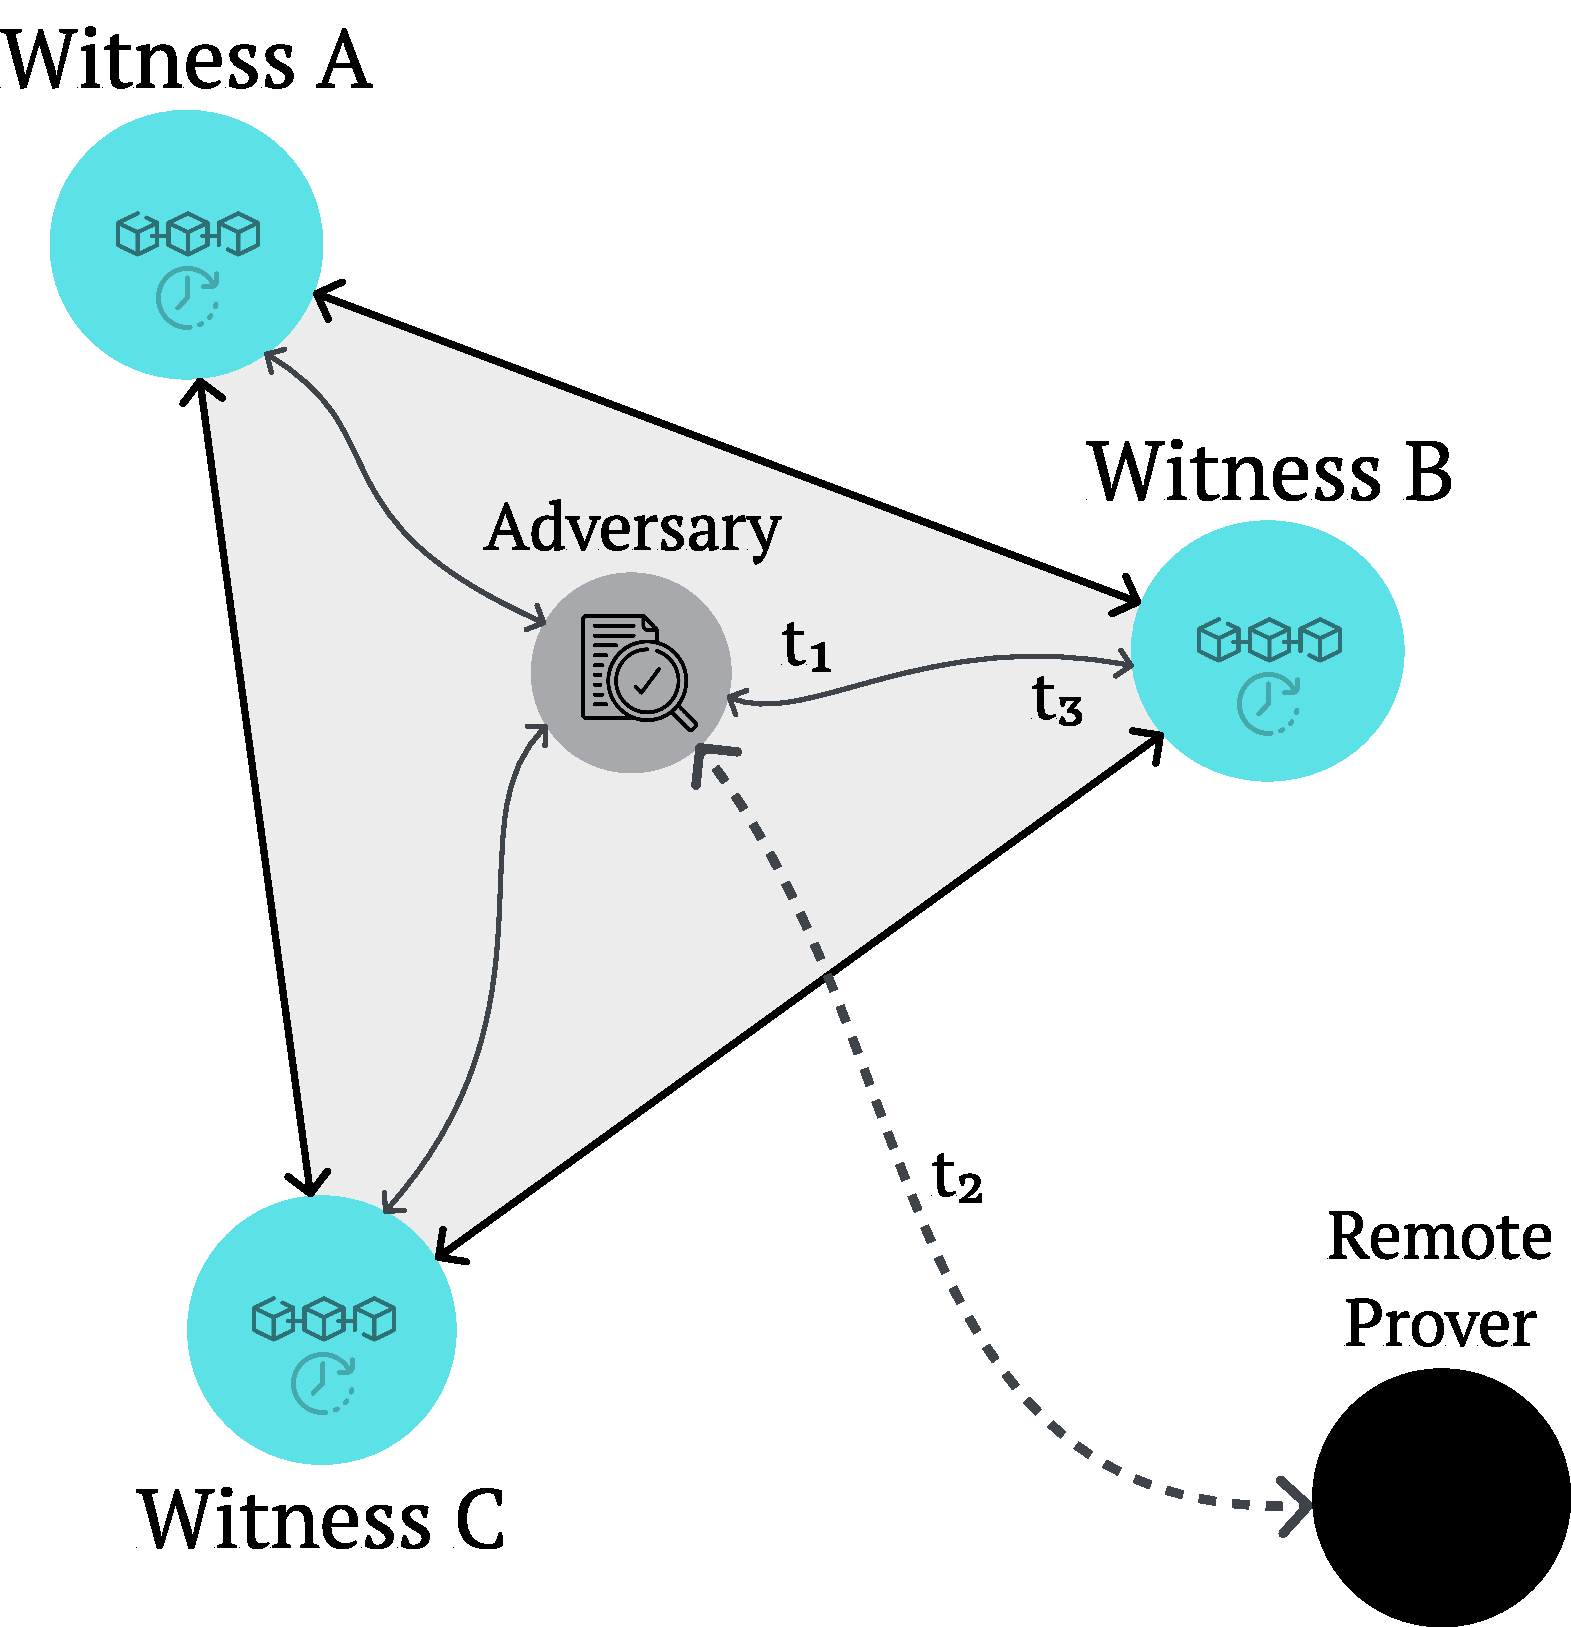
\includegraphics[width=0.6\textwidth]{pol-implementation-proxy-attack.pdf}
    \caption{A possible attack scenario, where a malicious prover is able to generate a \pol{} certificate without being nearby the witnesses. If $t_1 + t_2 + t_3 \leq T$, the adversary is able to act on behalf of the prover, synchronizing with the zone, asking the remote prover for a transaction signature, and generating a valid certificate \cite{nosouhi2020blockchain}.}
    \label{fig:pol-implementation:overview-proxy-wormhole}
    \end{center}
\end{figure}

The process of verifying the certificate validity was demonstrated along with the generation process, for testing purposes. However, the verification process can be independently automated as well, for instance, by making use of smart contracts. We have also developed an example of a smart contract, under the "proof-of-concept/src/pol-verifier" directory, that verifies the witnesses and prover signatures. Such contracts can be deployed in any private or public blockchain network, acting as decentralized verifiers and record keepers of \pol{} certificates. Nevertheless, it is important to note that the verification procedure is not limited to the use of smart contracts. The process can be performed by any verifier that has access to the entities' public keys and the \pol{} certificate, just like any typical digital signature verification, integrated with digital applications of all kinds.

% The pseudocode of such a contract is presented in Procedure~\ref{proc:block-hash-verifier}.

% \begin{procedure} [!h]
% 	\caption{BlockHashVerifier()} \label{proc:block-hash-verifier}
% 	\KwIn{Block Hash To Check $hashToCheck$}
% 	\KwResult{Transaction is Valid.}
% 	\BlankLine
%     $LastBlockHash \gets CurrentBlock.Hash$;
%     \BlankLine
%     \Return $hashToCheck == LastBlockHash$;
% 	%\eIf{error messages were found}{\Return \False\;}{\Return \True\;}
% \end{procedure}


% Geth choice for the Ethereum client
% Geth setup, including the genesis block, clique PoA vs PoW, etc.
% Geth run
% Prover client, requests, smart contract deployment failure, etc.
% Verifier example



\subsection{Measurements} \label{sec:proof-of-concept-results}

Along with the implementation of the proof-of-concept, we have conducted multiple experiments to evaluate the networking and computational performance of the proposed approach. The testbed was empirically hosted on a laptop with an AMD Ryzen 7 4700U CPU and 16 GB of RAM, running an x86-64 Linux 6.1.24-1-lts system. Every instance got assigned 1 GB of RAM and 2 virtual CPUs. 

The bridge interface, pooling all the mesh traffic exchanged between the tap interfaces, was the starting point for the networking measurements. All these interfaces had a maximum virtual bandwidth of 10 Mbit per second, assigned by the hosting system. The traffic was monitored using Wireshark\footnote{\url{https://www.wireshark.org/}}, and the metrics were collected throughout the various stages of the experiment, by listening to packets of different kinds, flowing through the bridge interface. Establishing the mesh network connectivity, the Ethernet frames belonging to the batman-adv protocol sized an average of 74 bytes, and the IPv4 related packets averaged at 278 bytes, presenting both protocols a seemingly linear throughput increase with the increase in the number of instances, as shown in Figure~\ref{fig:mesh-traffic}. 

\begin{figure} [h!]
    \centering
    \begin{subfigure}[b]{0.49\textwidth}
        \centering
        \begin{tikzpicture}
            \definecolor{line-color}{RGB}{92,255,230}
            \definecolor{line-color2}{RGB}{3,150,156}
            \begin{axis}[
                legend pos=outer north east,
                xlabel=instances (witnesses + prover),
                ylabel=throughput (Kbits/s),
                xmin=3, xmax=11,
                ymin=0.5, ymax=12,
                xtick={4,5,6,7,8,9,10},
                ytick={2, 4, 6, 8, 10, 12},
                grid=major,
                grid style={dashed},
                width=\textwidth
            ]
            
            \addplot[color=orange,mark=square] coordinates {
                (4,1.6) (5,3.0) (6,4.5) (7,5.9) (8,7.5) (9,9.3) (10,11)
                % (4,3.4) (5,5.7) (6,8.1) (7,11.2) (8,14) (9,16.8) (10,20)
            };
            \end{axis}
        \end{tikzpicture}
        \caption{Batman-adv traffic throughput.}
        \label{fig:y equals x}
    \end{subfigure}
    \hfill
    \begin{subfigure}[b]{0.49\textwidth}
        \centering
        \begin{tikzpicture}
            \definecolor{line-color}{RGB}{92,255,230}
            \definecolor{line-color2}{RGB}{3,150,156}
            \begin{axis}[
                legend pos=outer north east,
                xlabel=instances (witnesses + prover),
                % ylabel=throughput (Kbits/s),
                yticklabel pos=right,
                xmin=3, xmax=11,
                ymin=2, ymax=23,
                xtick={4,5,6,7,8,9,10},
                ytick={2, 4, 6, 8, 10, 12, 14, 16, 18, 20, 22},
                grid=major,
                grid style={dashed},
                width=\textwidth,
            ]
            
            \addplot[color=line-color2,mark=o] coordinates {
                (4,3.8) (5,6.8) (6,9.3) (7,12.7) (8,15.9) (9,19.1) (10,21.8)
            };        
            \end{axis}
        \end{tikzpicture}
        \caption{IPv4 traffic throughput.}
        \label{fig:three sin x}
    \end{subfigure}
    \caption{Average protocol throughput, measured in the bridge interface.}
    \label{fig:mesh-traffic}
\end{figure}

The Blockchain activity was also monitored, in order to observe the protocol behaviour, regarding the block generation and proposal phases. Figure~\ref{fig:blockchain-blocks-generation} captures the number of messages exchanged between the instances, during a time frame of typical protocol activity. The interval time between blocks, set to 10 seconds, corresponds to the higher peaks of TCP traffic, while the UDP traffic is more evenly distributed. This behaviour gets more pronounced as the number of instances increases, but the overall traffic is still proportionally low, with no significant impact on the network performance.

\begin{figure} [b!]
    \centering
    \begin{subfigure}[b]{\textwidth}
        \centering
        \vspace{-0.5cm}
        \pgfplotstableread[col sep=comma]{data/blockchain-blocks-generation-4-instances.csv}\datatable
        
        \begin{tikzpicture}
            \definecolor{line-color}{RGB}{3,150,156}
            \definecolor{line-color2}{RGB}{167,169,172}
            \begin{axis}[
                xlabel=time (s),
                ylabel=messages,
                xmin=-2, xmax=102,
                ymin=-5, ymax=40,
                ytick={0, 5, 10, 15, 20, 25, 30, 35, 40},
                grid=major,
                grid style={dashed},
                width=\textwidth,
                height=0.47\textwidth,
                legend pos=north west
            ]
        
            \addplot[mark=*,line-color] table[x=x,y=TCP]{\datatable};
            \addplot[mark=+,line-color2] table[x=x,y=UDP]{\datatable};
            \addplot[mark=o,orange] table[x=x,y=Batman-adv-orig]{\datatable};
        
            \legend{TCP, UDP, Batman-adv-orig}
        
            \end{axis}
        \end{tikzpicture}
        \caption{4 instances.}
        \label{fig:blockchain-blocks-generation-4-instances}
    \end{subfigure}
    \hfill
    \begin{subfigure}[b]{\textwidth}
        \centering
        \pgfplotstableread[col sep=comma]{data/blockchain-blocks-generation-8-instances.csv}\datatable
        
        \begin{tikzpicture}
            \definecolor{line-color}{RGB}{3,150,156}
            \definecolor{line-color2}{RGB}{167,169,172}
            \begin{axis}[
                xlabel=time (s),
                ylabel=messages,
                xmin=-2, xmax=102,
                ymin=-50, ymax=300,
                ytick={0, 50, 100, 150, 200, 250, 300},
                grid=major,
                grid style={dashed},
                width=\textwidth,
                height=0.47\textwidth,
                legend pos=north west
            ]
        
            \addplot[mark=*,line-color] table[x=x,y=TCP]{\datatable};
            \addplot[mark=+,line-color2] table[x=x,y=UDP]{\datatable};
            \addplot[mark=o,orange] table[x=x,y=Batman-adv-orig]{\datatable};
        
            \legend{TCP, UDP, Batman-adv-orig}
        
            \end{axis}
        \end{tikzpicture}
        \caption{8 instances.}
        \label{fig:blockchain-blocks-generation-8-instances}
    \end{subfigure}
    \caption{The network activity, with a block time of 10 seconds.}
    \vspace{-0.5cm}
    \label{fig:blockchain-blocks-generation}
\end{figure}

Both CPU and RAM usages were also continuously measured across the whole experiment. The two virtual cores of each instance saw the CPU usage averaging at 2\%, peaking at 20\% when the prover would interact with a witness, or vice versa, in order to produce a \pol{} certificate. The overall RAM usage did not go beyond 200 MB. These numbers are in line with the expected behaviour of the protocol, running the PoA consensus algorithm, as a lightweight mechanism that may not require much computational power, suitable and adaptable to resource-constrained environments. The PoW consensus algorithm, on the other hand, would require a much higher and variable computational power, that would be difficult to predict and control, since it is not only manually configured, but dependent, as well, on the dynamic difficulty adjustment mechanism, in order to meet a fixed block time. Nevertheless, both protocols should present similar network traffic patterns. In terms of storage, the disk space used did not exceed 65 MB, for the entire file system.

The proof generation process did not possess enough relevancy for time measurement purposes. Its execution speed, during the transaction creation, signing, and broadcasting phases is highly dependent on the running environment, and not limited to the showcased implementation. It can be effectively optimized in multiple ways, using different libraries, programming languages, or parallelization techniques. Moreover, the total execution time is ultimately bounded to the block time, since the prover needs to wait a maximum of $T$ units of time for the generation of the new block that may contain its transaction. The proof generation process is also not a bottleneck in the protocol, as it is not a part of the consensus mechanism, and may be executed in parallel with the other protocol activities. The certificate assembly and verification processes can, as well, be performed later and asynchronously. Nonetheless, the success rate of the generation of \pol{} certificates may still be assessed. For such experiment, we adjusted the interval time between blocks and measured the number of valid \pol{} certificates. A similar test was conducted by Nosouhi et al. \cite{nosouhi2020blockchain}, targeting the effectiveness of their protocol against prover-prover collusions, or proxy and wormhole attacks. The test is still dependent on the characteristics of the running environment, but the results sustain the conclusion that the block time is a crucial parameter in the protocol. Figure~\ref{fig:block-time-success-rate} shows a direct relation between the block time and the success rate in generating valid certificates. The higher the block time, the lower the failures. The consequences of such relation are twofold. A more permissive block time allows for a lower number of invalid certificates, but also for a higher probability of witnessing malicious activity, such as collusions between adversaries and remote provers, as explained in Figure~\ref{fig:pol-implementation:overview-proxy-wormhole}. The block time is, therefore, a trade-off between the two, and should be carefully adjusted to the running environment. Further reasoning is still needed, to deeper assess the impact of this heuristic, or to propose a more robust solution.

\begin{figure} [h!]
    \begin{center}
        \begin{tikzpicture}
            \definecolor{line-color2}{RGB}{3,150,156}
            \begin{axis}[
                xlabel=block time (s),
                ylabel=success rate (\%),
                xmin=0, xmax=11,
                ymin=-5, ymax=100,
                xtick={0, 1, 2, 3, 4, 5, 6, 7, 8, 9, 10},
                ytick={0, 25, 50, 75, 100},
                grid=major,
                grid style={dashed},
                width=0.8\textwidth,
                height=0.4\textwidth,
            ]

            \addplot[color=line-color2,mark=o] coordinates {
                (1, 2) (2, 2.7) (3, 7.4) (4, 25.3) (5, 43.1) (6, 68.4) (7, 80.2) (8, 87.0) (9, 91.2) (10, 94.2)
            };
            \end{axis}
        \end{tikzpicture}
        \caption{The success rate of the generation of \pol{} certificates.}
        \label{fig:block-time-success-rate}
    \end{center}
\end{figure}

In retrospective, the main goal of achieving a fully functional proof-of-concept for the \pol{} protocol was, indeed, reached. We have fulfilled the requirements proposed in Chapter~\ref{sec:protocol-fundamentals} and made a demonstration possible. The protocol was implemented in a distributed setting, with a modular network architecture, and a clear separation of concerns between the different stages. We have also engineered the solution with enough flexibility, allowing for an easy integration of new components, or the replacement or tuning of the existing ones, in order to adapt to different environments, or to improve the overall performance. Further measurement considerations, along with the demonstration in a physical environment, are already in our horizon. 

The thesis work extended over several months, spanning multiple semesters and encompassing several distinct stages and significant milestones. The first semester was primarily dedicated to researching and reviewing permissionless consensus mechanisms, which led to prototyping and demonstrating an ad-hoc consensus protocol. This work accounted for approximately 250 hours of effort. In the second semester, the focus was on researching the \pol{} paradigm and the protocol's design. The theoretical work of reviewing existing solutions, dissecting the paradigm, and proposing a new protocol, took approximately 350 hours of effort. This work was interleaved with the implementation of the proof-of-concept. Multiple weeks were spent on trials with the image building, the network setup, the deployment in physical devices, and the configuration of the consensus protocol. The practical work accounted for approximately 400 hours of total effort, including, as well, the successes reported. The thesis writing took place in both semesters and is included in the estimations. The work is still ongoing, and the next chapter will address the overall conclusions and future work that is to be conducted to improve and expand this \pol{} protocol.

%%%%%%%%%%%%%%%%%%%%%%%%%%%%%%%%%%%%%%%%%%%%%%%%%%%%%%%%%%%%%%%%%%%%%%%%%%%%%%%%

% \begin{figure}[h!]
%     \begin{center}
% \begin{tikzpicture}
%     \definecolor{line-color}{RGB}{92,255,230}
%     \definecolor{line-color2}{RGB}{3,150,156}
%     \begin{axis}[
%         legend pos=outer north east,
%         xlabel=number of instances (witnesses + prover),
%         ylabel=throughput (Kbits/s),
%         xmin=3, xmax=11,
%         ymin=1, ymax=12,
%         xtick={4,5,6,7,8,9,10},
%         ytick={2, 4, 6, 8, 10, 12},
%         grid=major,
%         grid style={dashed},
%         width=0.8\textwidth,
%         height=0.4\textwidth,
%     ]
    
%     \addplot[color=orange,mark=square] coordinates {
%         (4,1.8) (5,3.0) (6,4.2) (7,5.6) (8,7.5) (9,9.0) (10,11)
%         % (4,3.4) (5,5.7) (6,8.1) (7,11.2) (8,14) (9,16.8) (10,20)
%     };
%     % \addlegendentry{batman-adv}

%     % \addplot[color=line-color2,mark=o] coordinates {
%     %     (4,4.5) (5,6.8) (6,9.3) (7,12.7) (8,15.9) (9,19.1) (10,21.8)
%     % };
%     % \addlegendentry{IPv4}

%     \end{axis}
% \end{tikzpicture}
% \caption{Average batman-adv traffic throughput, measured on the bridge interface.}
% \label{fig:mesh-traffic}
% \end{center}
% \end{figure}

% \begin{figure}[h!]
%     \begin{center}
% \begin{tikzpicture}
%     \definecolor{line-color}{RGB}{92,255,230}
%     \definecolor{line-color2}{RGB}{3,150,156}
%     \begin{axis}[
%         legend pos=outer north east,
%         xlabel=number of instances (witnesses + prover),
%         ylabel=throughput (Kbits/s),
%         xmin=3, xmax=11,
%         ymin=2.5, ymax=22.5,
%         xtick={4,5,6,7,8,9,10},
%         ytick={2, 4, 6, 8, 10, 12, 14, 16, 18, 20, 22},
%         grid=major,
%         grid style={dashed},
%         width=0.8\textwidth,
%         height=0.4\textwidth,
%     ]
    
%     \addplot[color=line-color2,mark=o] coordinates {
%         (4,4.5) (5,6.8) (6,9.3) (7,12.7) (8,15.9) (9,19.1) (10,21.8)
%     };
%     \addlegendentry{IPv4}

%     \end{axis}
% \end{tikzpicture}
% \caption{Average batman-adv traffic throughput, measured on the bridge interface.}
% \label{fig:mesh-traffic}
% \end{center}
% \end{figure}

% \begin{figure} [h!]
% \begin{tabular}{c c}
% \begin{minipage}{0.50\textwidth}
%     \begin{center}
%         \begin{tikzpicture}
%             \definecolor{line-color}{RGB}{92,255,230}
%             \definecolor{line-color2}{RGB}{3,150,156}
%             \begin{axis}[
%                 legend pos=outer north east,
%                 xlabel=instances (witnesses + prover),
%                 ylabel=throughput (Kbits/s),
%                 xmin=3, xmax=11,
%                 ymin=1, ymax=12,
%                 xtick={4,5,6,7,8,9,10},
%                 ytick={2, 4, 6, 8, 10, 12},
%                 grid=major,
%                 grid style={dashed},
%                 width=\textwidth,
%                 height=0.8\textwidth,
%             ]
            
%             \addplot[color=orange,mark=square] coordinates {
%                 (4,1.8) (5,3.0) (6,4.2) (7,5.6) (8,7.5) (9,9.0) (10,11)
%                 % (4,3.4) (5,5.7) (6,8.1) (7,11.2) (8,14) (9,16.8) (10,20)
%             };
%             \end{axis}
%         \end{tikzpicture}
%         \caption{(a) Average batman-adv traffic throughput.}
%         % \label{fig:mesh-traffic}
%         \end{center}
% \end{minipage}
% &
% \begin{minipage}{0.50\textwidth}

%     \begin{center}
%         \begin{tikzpicture}
%             \definecolor{line-color}{RGB}{92,255,230}
%             \definecolor{line-color2}{RGB}{3,150,156}
%             \begin{axis}[
%                 legend pos=outer north east,
%                 xlabel=instances (witnesses + prover),
%                 % ylabel=throughput (Kbits/s),
%                 xmin=3, xmax=11,
%                 ymin=2.5, ymax=22.5,
%                 xtick={4,5,6,7,8,9,10},
%                 ytick={2, 4, 6, 8, 10, 12, 14, 16, 18, 20, 22},
%                 grid=major,
%                 grid style={dashed},
%                 width=\textwidth,
%                 height=0.8\textwidth,
%             ]
            
%             \addplot[color=line-color2,mark=o] coordinates {
%                 (4,4.5) (5,6.8) (6,9.3) (7,12.7) (8,15.9) (9,19.1) (10,21.8)
%             };        
%             \end{axis}
%         \end{tikzpicture}
%         \caption{(a) Average IPv4 traffic throughput.}
%         \end{center}

% \end{minipage}
% \end{tabular}
% \caption{Example how to put two figures parallel to each other.}
% \label{fig:LCA_2_solutions}
% \end{figure}

% \begin{figure}[h!]
% \pgfplotstableread[col sep=comma]{data/br-qemu.csv}\datatable

% \begin{tikzpicture}
%     \definecolor{line-color}{RGB}{3,150,156}
%     \definecolor{line-color2}{RGB}{167,169,172}
%     \begin{axis}[
%         xlabel=time (s),
%         ylabel=throughput (Bits/s),
%         xmin=10, xmax=20,
%         ymin=-100, ymax=1300,
%         ytick={0,200,400,600,800,1000,1200},
%         grid=major,
%         grid style={dashed},
%         width=\textwidth,
%         height=0.5\textwidth,
%     ]

%     \addplot[mark=*,line-color2] table[x=Interval start,y=prover 1]{\datatable};
%     \addplot[mark=+,line-color] table[x=Interval start,y=witness 1]{\datatable};
%     \addplot[mark=x,line-color] table[x=Interval start,y=witness 2]{\datatable};
%     \addplot[mark=o,line-color] table[x=Interval start,y=witness 3]{\datatable};

%     \legend{prover, witness 1, witness 2, witness 3}

%     \end{axis}
% \end{tikzpicture}
% \caption{Ethernet traffic throughput, measured on the bridge interface.}
% \label{fig:mesh-traffic-3-witnesses}
% \end{figure}


% \begin{figure}[h!]
% \pgfplotstableread[col sep=comma]{data/blockchain-blocks-generation-8-instances.csv}\datatable

% \begin{tikzpicture}
%     \definecolor{line-color}{RGB}{3,150,156}
%     \definecolor{line-color2}{RGB}{167,169,172}
%     \begin{axis}[
%         xlabel=time (s),
%         ylabel=messages,
%         xmin=-2, xmax=102,
%         ymin=-50, ymax=300,
%         ytick={0, 50, 100, 150, 200, 250, 300},
%         grid=major,
%         grid style={dashed},
%         width=\textwidth,
%         height=0.5\textwidth,
%         legend pos=north west
%     ]

%     \addplot[mark=*,line-color] table[x=x,y=TCP]{\datatable};
%     \addplot[mark=+,line-color2] table[x=x,y=UDP]{\datatable};
%     \addplot[mark=o,orange] table[x=x,y=Batman-adv-orig]{\datatable};

%     \legend{TCP, UDP, Batman-adv-orig}

%     \end{axis}
% \end{tikzpicture}
% \caption{The network activity, with a block time of 10 seconds.}
% \label{fig:blockchain-blocks-generation}
% \end{figure}


% AMD Ryzen 7 4700U with Radeon Graphics (with SSE4.2)
% Linux 6.1.24-1-lts


\newpage

\section{Conclusion} \label{sec:conclusion}

This thesis developed, implemented, and evaluated an AI-powered, web-based Mini-Mental State Examination (MMSE) application, introducing an innovative approach to cognitive assessment. The research addressed longstanding challenges in neuropsychological testing by integrating advanced AI technologies, such as Large Language Models (LLMs) including Llama 3.1 and ChatGPT 4.0, with traditional assessment methods.
The study's primary findings underscore the significant potential of AI-enhanced cognitive assessment tools:
\begin{enumerate}
\item \textbf{Accuracy and Consistency}: The Llama 3.1 70B model achieved a 92.9 percent success rate in confirming the correctness of responses within a specific test suite, demonstrating its potential to enhance the reliability of cognitive assessments.
\item \textbf{Enhanced Accessibility}: The web-based application transcended geographical barriers, making cognitive assessments more accessible to underserved populations and facilitating remote evaluations.
\item \textbf{Standardization}: Automated scoring and analysis contributed to more consistent assessment processes across varied settings, reducing the variability associated with human scoring.
\item \textbf{Adaptability}: AI models enabled dynamic adjustments in test difficulty and personalization, potentially increasing sensitivity to subtle cognitive changes.
\end{enumerate}
However, several challenges remain:
\begin{enumerate}
\item \textbf{Response Time}: Optimizing the balance between accuracy and speed, particularly with the Llama 3.1 model, is necessary. The current web-based version requires longer administration times compared to traditional methods.
\item \textbf{Data Privacy and Security}: Safeguarding sensitive healthcare data within AI systems is critical and requires robust measures.
\item \textbf{Accessibility for Older Adults}: Bridging the digital divide among older populations is essential for the widespread adoption of this technology.
\item \textbf{Ethical Considerations}: The use of AI in cognitive assessments raises ethical concerns regarding fairness, transparency, and potential bias.
\end{enumerate}
This research contributed significantly to the evolving intersection of AI and healthcare diagnostics. Demonstrating the feasibility of AI-powered cognitive assessments established a foundation for future research and development in this critical area.
Future research should focus on:
\begin{enumerate}
\item \textbf{Larger-Scale Validation}: Conducting studies with more extensive and diverse samples to confirm the effectiveness and reliability of the AI-powered MMSE.
\item \textbf{Longitudinal Studies}: Evaluating the utility of the AI-powered MMSE in tracking cognitive changes over time.
\item \textbf{Cross-Cultural Adaptation}: Expanding support for multiple languages and cultural contexts to enhance global applicability.
\item \textbf{Integration with Health Records}: Exploring seamless integration with electronic health record systems to increase clinical utility.
\item \textbf{Advanced AI Techniques}: Investigating sophisticated AI approaches, such as federated learning, to address data privacy concerns.
\end{enumerate}
In conclusion, this research marked a significant step toward integrating AI into cognitive health assessments. While the findings are preliminary, the potential benefits of enhanced standardization, accessibility, and efficiency are considerable. As AI technologies continue to evolve and ethical and practical concerns are addressed, the future holds promise for improved cognitive assessments, leading to earlier detection and better management of cognitive decline. Continued research and development in this area will likely improve patient outcomes and support healthcare providers in delivering high-quality care.

\subsection*{Acknowledgments}
The author sincerely thanks Dr. Mohamad Gharib for his expert guidance and invaluable support throughout this research. Thanks are due to the University of Tartu's Institute of Computer Science for providing an excellent academic environment and resources. Eduardo Brito's advice and shared ideas merit special recognition.

This work benefited from various technical tools and AI assistants, as detailed in Appendix \ref{appendix:writing-workflow}. PlantUML facilitated diagram creation.

Gratitude is extended to the experts who tested the application and provided feedback, and to family and friends for their unwavering support. This thesis demonstrates the power of collaborative academic research and supportive communities in education.

This version maintains the essential acknowledgments, includes the reference to the appendix for more detailed information about the tools used, and remains concise and appropriate for an academic thesis.

\newpage

% BibTeX bibliography
\bibliographystyle{ieeetr} %plain=[1], alpha=[BGZ09]
\bibliography{unitartucs-thesis}
\addcontentsline{toc}{section}{\refname}

\newpage

\appendix

\section*{Appendix}
\addcontentsline{toc}{section}{Appendix}

\newcounter{appendixcounter}
\renewcommand{\theappendixcounter}{\Roman{appendixcounter}}

%%%%%%%%%%%%%%%%%%%%%%%%%%%%%%%%%%%%%%%%%%%%%%%%%%%%%%%%%%%%%%%%%%%%%%%%%%%%%%%%%%%%%%%%%%%%%%%%

\refstepcounter{appendixcounter}

\subsection*{\Roman{appendixcounter}. Repository} \label{appendix:repository}

\addcontentsline{toc}{subsection}{I. Repository}

The source code, documentation, and other materials produced for this thesis are available in the following repositories:
\begin{itemize}
    \item Master's Thesis: \url{https://github.com/ktenman/master-thesis-ut}
    \item MMSE Prototype App: \url{https://github.com/ktenman/mmse-app}
\end{itemize}

%%%%%%%%%%%%%%%%%%%%%%%%%%%%%%%%%%%%%%%%%%%%%%%%%%%%%%%%%%%%%%%%%%%%%%%%%%%%%%%%%%%%%%%%%%%%%%%%

\refstepcounter{appendixcounter}

\subsection*{\Roman{appendixcounter}. Licence}

\addcontentsline{toc}{subsection}{II. Licence}

\subsubsection*{Non-exclusive license to reproduce the thesis and make the thesis public}

I, \textbf{\authorname}, %author's name
%   \licencehint{10mm}{author's name}

\begin{enumerate}
\item
herewith grant the University of Tartu a free permit (non-exclusive license) to
reproduce for the purpose of preservation, including for adding to the DSpace digital archives until the expiry of the term of copyright,
\par
\textbf{\thesistitle}, %
%   \licencehint{10mm}{title of thesis}
\par
supervised by \supervisor. %supervisor's name
%   \licencehint{10mm}{supervisor's name}
\item
I grant the University of Tartu a permit to perform the work specified in p. 1 available to the public via the web environment of the University of Tartu, including via the DSpace digital archives, under the Creative Commons license CC BY NC ND 3.0, which allows, by giving appropriate credit to the author, to reproduce, distribute the work, and communicate it to the public, and prohibits the creation of derivative works and any commercial use of the work until the expiry of the term of copyright.
\item
I am aware of the fact that the author retains the rights specified in p. 1 and 2.
\item
I certify that granting the nonexclusive license does not infringe on other persons' intellectual property rights or rights arising from the personal data protection legislation. 
\end{enumerate}

\noindent
Konstantin Tenman\\ %author's name
\textbf{\textsl{13/08/2024}}

%%%%%%%%%%%%%%%%%%%%%%%%%%%%%%%%%%%%%%%%%%%%%%%%%%%%%%%%%%%%%%%%%%%%%%%%%%%%%%%%%%%%%%%%%%%%%%%%
\newpage
\refstepcounter{appendixcounter}

\subsection*{\Roman{appendixcounter}. Traditional Mini-Mental State Examination (MMSE)} \label{appendix:mmse}

\addcontentsline{toc}{subsection}{III. Traditional Mini-Mental State Examination (MMSE)}

The following table details the tasks involved in the traditional Mini-Mental State Examination (MMSE):

\begin{table}[h!]
\centering
\caption{Traditional Mini-Mental State Examination (MMSE)}
\begin{tabular}{|p{0.3\textwidth}|p{0.6\textwidth}|}
\hline
\textbf{Task} & \textbf{Description} \\
\hline
Orientation to Time (5 points) & Assess the person's awareness of the current date and time. Questions include the date, day of the week, month, and year. \\
\hline
Orientation to Place (5 points) & Assess the individual's awareness of their current location. Questions include the type of building, the floor, the city, etc. \\
\hline
Registration of Three Objects (3 points) & Test immediate memory and attention by having the person repeat three unrelated objects. \\
\hline
Attention and Calculation (5 points) & Evaluate attention and working memory by having the person subtract 7 from 100 and continue subtracting 7, or spell "world" backward. \\
\hline
Recall of Three Objects (3 points) & Test the ability to store and recall information after a short delay by having the person recall the three objects from the registration task. \\
\hline
Naming (2 points) & Test semantic memory and language production by having the person name two objects (like a pencil and a watch). \\
\hline
Repetition (1 point) & Test language production and verbal comprehension by having the person repeat a phrase like "No ifs, ands, or buts". \\
\hline
Three-Stage Command (3 points) & Assess the ability to understand and follow complex instructions by having the person follow a three-step command. \\
\hline
Reading (1 point) & Test reading comprehension by having the person read and follow a written command like "Close your eyes". \\
\hline
Writing (1 point) & Assess writing ability by having the person write a sentence. \\
\hline
Drawing (1 point) & Assess visuospatial abilities by having the person copy a complex diagram like two intersecting pentagons. \\
\hline
\end{tabular}
\label{tab:traditional-mmse}
\end{table}

%%%%%%%%%%%%%%%%%%%%%%%%%%%%%%%%%%%%%%%%%%%%%%%%%%%%%%%%%%%%%%%%%%%%%%%%%%%%%%%%%%%%%%%%%%%%%%%%



\newpage
\refstepcounter{appendixcounter}

\subsection*{\Roman{appendixcounter}. Participant Consent Form} \label{appendix:concent}


\section*{Participant Consent Form for AI-Powered and Traditional MMSE Tool Testing}
\noindent
You are invited to participate in a research study to evaluate both the AI-powered MMSE tool and traditional paper-based MMSE tests. The purpose of this study is to assess the usability, accuracy, and effectiveness of the AI-powered tool in comparison to traditional methods of cognitive assessment. Your participation will involve completing a series of cognitive assessments using both the AI-powered MMSE tool and traditional paper-based MMSE tests.

\vspace{0.5cm}

\noindent
\textbf{Confidentiality and Data Protection}

\begin{itemize}
    \item Your participation in this study is voluntary, and you may withdraw at any time without penalty.
    \item All data collected during the study will be kept confidential and will be anonymized.
    \item The data will be used solely for the purposes of this research and will be removed from our records after the analysis is complete.
    \item Your identity will not be revealed in any reports or publications resulting from this study.
\end{itemize}

\vspace{0.5cm}

\noindent
\textbf{Consent}

\begin{itemize}
    \item I understand the purpose of this study and what is expected of me as a participant.
    \item I understand that my participation is voluntary and that I may withdraw at any time without penalty.
    \item I understand that my data will be kept confidential and will be removed after the analysis is complete.
    \item I understand that I will be completing both AI-powered and traditional paper-based MMSE tests.
    \item I agree to participate in this study.
\end{itemize}

\vspace{0.5cm}

\noindent
\textbf{Participant's Signature:} \underline{\hspace{8cm}}

\noindent
\textbf{Participant's Printed Name:} \underline{\hspace{8cm}}

\noindent
\textbf{Date:} \underline{\hspace{8cm}}

\vspace{0.5cm}

\noindent
\textbf{Researcher’s Contact Information}

\noindent
If you have any questions or concerns about this study, please contact:

\begin{tabbing}
\hspace{3cm} \= Name: \hspace{1cm} \= [Your Name] \\
\> Email: \> [Your Email] \\
\> Phone: \> [Your Phone Number]
\end{tabbing}


\newpage
\refstepcounter{appendixcounter}

\subsection*{\Roman{appendixcounter}. Writing Workflow} \label{appendix:writing-workflow}

\addcontentsline{toc}{subsection}{IV. Writing Workflow}

The author utilized a comprehensive set of tools and environments, which are documented here to illustrate the workflow.

The writing process relied on \LaTeX{}, a robust document preparation system that emphasized content over formatting. IntelliJ IDEA and Overleaf were the primary development environments, with Overleaf selected for its collaborative and template management features.

Version control was managed with Git, with GitHub hosting the remote repository containing the \LaTeX{} source files, MMSE prototype app code, and associated documentation, as detailed in Appendix~\ref{appendix:repository}. GitHub Copilot assisted with code completion and debugging.

AI tools, including ChatGPT, Grammarly, and Claude AI, were employed to summarize, rewrite, contextualize, and refine content. Grammarly enhanced language precision. Diagramming was done using PlantUML, which facilitated the creation of precise and standardized diagrams.



\end{document}

